% Retoca las líneas marcadas con TODO según las necesidades

\documentclass[oneside,a4paper,12pt]{book} % TODO: cambia "oneside" por "twoside" a la hora de imprimirlo

\usepackage[spanish]{babel}
\usepackage[utf8]{inputenc}
\usepackage{geometry}
\usepackage{makeidx}
\usepackage{url}
\usepackage{graphicx}
\usepackage{color}
\usepackage{caption}
\usepackage{acronym}
\usepackage{hyphenat}
\usepackage{a4wide}
\usepackage[normalsize]{subfigure}
\usepackage{float}
\usepackage{titlesec}
\usepackage[Lenny]{fncychap}
\usepackage{listings} % para poder hacer uso de "listings" propios (p.ej. códigos)
\usepackage{eurosym} % para poder usar el símbolo del euro con \euro {xx}
\usepackage{hyperref} % TODO: añade la opción hidelinks para imprimirlo (los enlaces no aparecerán resaltados)
% EXPRESIONES MATEMÁTICAS
\usepackage{amsmath,amssymb,amsfonts,amsthm}
% Para que no parta las palabras
\pretolerance=10000

\usepackage{afterpage}
\newcommand\blankpage{%
    \null
    \thispagestyle{empty}%
    \addtocounter{page}{-1}%
    \newpage}

\newcommand{\bigrule}{\titlerule[0.5mm]} \titleformat{\chapter}[display] % cambiamos el formato de los capítulos
{\bfseries\Huge} % por defecto se usaron caracteres de tamaño huge en negrita
{% contenido de la etiqueta 
\titlerule % línea horizontal 
\filright % texto alineado a la derecha 
\Large\chaptertitlename\ % capítulo e índice en tamaño large
\Large % en lugar de 
\Huge \Large\thechapter} 
{0mm} % espacio mínimo entre etiqueta y cuerpo
{\filright} % texto del cuerpo alineado a la derecha
[\vspace{0.5mm} \bigrule] % después del cuerpo, dejar espacio vertical y trazar línea horizontal gruesa
\geometry{a4paper, left=3.5cm, right=2cm, top=3cm, bottom=2cm, headsep=1.5cm}

% Estilos para ilustrar códigos:
\definecolor{code_green}{rgb}{0,0.6,0}
\definecolor{code_gray}{rgb}{0.5,0.5,0.5}
\definecolor{code_mauve}{rgb}{0.58,0,0.82}

\lstset{frame=tb,
  language=C,
  aboveskip=3mm,
  belowskip=3mm,
  showstringspaces=false,
  columns=flexible,
  basicstyle={\small\ttfamily},
  numbers=none,
  numberstyle=\tiny\color{code_gray},
  keywordstyle=\color{blue},
  commentstyle=\color{code_green},
  stringstyle=\color{code_mauve},
  breaklines=true,
  breakatwhitespace=true,
  tabsize=3
}

\lstset{frame=tb,
  language=C++,
  aboveskip=3mm,
  belowskip=3mm,
  showstringspaces=false,
  columns=flexible,
  basicstyle={\small\ttfamily},
  numbers=none,
  numberstyle=\tiny\color{code_gray},
  keywordstyle=\color{blue},
  commentstyle=\color{code_green},
  stringstyle=\color{code_mauve},
  breaklines=true,
  breakatwhitespace=true,
  tabsize=3
}

\lstset{frame=tb,
  language=Python,
  aboveskip=3mm,
  belowskip=3mm,
  showstringspaces=false,
  columns=flexible,
  basicstyle={\small\ttfamily},
  numbers=none,
  numberstyle=\tiny\color{code_gray},
  keywordstyle=\color{blue},
  commentstyle=\color{code_green},
  stringstyle=\color{code_mauve},
  breaklines=true,
  breakatwhitespace=true,
  tabsize=3
}

% Definición de mis propios tipos: Códigos, Ecuaciones y Tablas
\DeclareCaptionType{code}[Código][Listado de códigos]
\DeclareCaptionType{myequation}[Ecuación][Listado de ecuaciones]

% TODO: especifica las reglas de separación que consideres. Algunos ejemplos:
\hyphenation{fuer-tes}
\hyphenation{mul-ti-ca-pa}
\hyphenation{res-pues-ta}
\hyphenation{di-fe-ren-tes}
\hyphenation{de-sa-rro-lla-dos}
\hyphenation{re-pre-sen-tan-do}

 % archivo de configuracion de estilo

\usepackage{array}
\usepackage{multirow}
\usepackage{natbib}
\usepackage{subcaption}
\usepackage{graphicx}
\usepackage{listings}

\hypersetup{
    colorlinks=true,
    linkcolor=black,
    urlcolor=black,
    citecolor=black
}

\makeindex

\begin{document}
\baselineskip 1.35\baselineskip

\frontmatter

\thispagestyle{empty}

\begin{titlepage}
	\begin{center}
		\vspace*{3mm}
		\begin{center}
			
\includegraphics[width=0.4\linewidth]{imagenes/cap1/logo_urjc}
		\end{center}
		\vspace{6.0mm}
		
		\fontsize{15.5}{14}\selectfont ESCUELA DE INGENIERÍA DE FUENLABRADA
		\vspace{13mm}
		
		\fontsize{14}{14}\selectfont GRADO EN INGENIERÍA DE ROBÓTICA SOFTWARE
		
		\vspace{70pt}
		
		\fontfamily{lmss}\fontsize{15.7}{14}\selectfont \textbf{TRABAJO FIN DE GRADO} 
		
		\vspace{20mm}
		\begin{LARGE}
			Conducción autonoma en CARLA \\
			 con adaptación al tráfico  \\
			basado en aprendizaje por refuerzo
		\end{LARGE}
		
		\vspace{20mm}
		
		\begin{large}
			Autor: Juan Camilo Carmona Sánchez
			
			Tutor: Dr. Roberto Calvo Palomino
			
			\vspace{10mm}
		\end{large}
		\begin{normalsize}
			Curso académico 2023/2024		
		\end{normalsize}
		\vspace{10mm}
		
	\end{center}
	
\end{titlepage}

\thispagestyle{empty}


\cleardoublepage

\chapter*{Agradecimientos}

Quiero agradecer Primero que nada a mi Madre, la única persona que ha estado conmigo a lo largo de toda mi vida, la persona que yo mas quiero y a la que le debo la que le debo todo lo que soy hoy en día. Gracias Mami por siempre haberme apoyado y ayudado a conseguir todas las metas que me he propuesto por haberme educado e inculcado todos los valores que hoy en día para mi son tan importantes y por haberlo sacrificado todo para que yo pudiera llegar hasta aquí.

\bigskip

En segundo lugar quiero agradecer a mi Padre, Javier, por haber sido otro de los apoyos fundamentales a lo largo de toda mi vida y haberme brindado toda la educación tanto académica como moral para ser una persona de bien, por haberme cuidado y criado y haberme ayudado a llegar donde estoy ahora mismo.

\bigskip

También quiero agradecer a mi Abuela. Una de las personas más importantes para mi en este mundo y que siempre me ha cuidado, me ha querido y me ha brindado cualquier cosa que he necesitado. Gracias Tita.

\bigskip

Finalmente quiero agradecer a mi abuelo, la persona que yo más he admirado y querido en toda mi vida y la razón por la que siempre he querido ser ingeniero. Gracias Chinche por fin lo he logrado estoy seguro que estarías orgulloso.

\bigskip

Y por supuesto quiero agradecerme a mi mismo, por haberme esforzado y haber superado todos los obstáculos que se han ido presentando en el camino, por nunca haberme rendido a pesar de todos los momento en los que parecía que no podría lograrlo y por haber conseguido el sueño de toda mi vida, convertirme en ingeniero.
\bigskip

\begin{flushright}
		\par
		\vspace{1.0 cm}
		Madrid, 12 de octubre de 2023\\ %\today
		\emph{Juan Camilo Carmona Sánchez}
\end{flushright}

\thispagestyle{empty}

\cleardoublepage

\chapter*{Resumen\markboth{Resumen}{Resumen}}

La conducción autónoma se refiere al uso de sistemas informáticos y tecnologías de inteligencia artificial para permitir que un vehículo se desplace de un lugar a otro sin necesidad de la intervención humana. esta tecnología representa una de las revoluciones tecnológicas más grandes y significativas del siglo XXI. Los pequeños avances que se logran día a día en este ámbito nos ponen un poquito más cerca de un futuro que tiempo atrás parecía utópico e inalcanzable, en el que las personas podremos pasarle el testigo de la movilizacion humana a las máquinas y dejarlas encargadas por completo de nuestro transporte a lo largo de ciudades, países y continentes.
\bigskip

La conducción autónoma se encuentra actualmente en una fase intermedia de su desarrollo, con numerosos avances y despliegues parciales que ofrecen un vistazo al futuro de la movilidad. A pesar de que todavía no hemos alcanzado un nivel de autonomía completo en todas las situaciones y entornos, empresas líderes en el sector como Tesla, Waymo y Cruise ya han introducido sistemas avanzados de asistencia al conductor y, en algunos casos, servicios de transporte sin conductor en áreas específicas. Aunque estas implementaciones actuales suelen requerir la supervisión humana y están principalmente limitadas a escenarios y ubicaciones bien definidos.

\bigskip

A pesar del estado actual de esta tecnología la visión de futuro para los vehículos autónomos es ambiciosa. Se espera que las innovaciones en \ac{IA}, sensores y computación contribuyan a superar las limitaciones actuales. La meta es alcanzar un nivel de autonomía en el que los vehículos puedan navegar de forma segura y eficiente en cualquier entorno o condición climática, sin necesidad de intervención humana. Este avance no solo cambiaría la forma en que nos movemos, sino que también tendría implicaciones profundas en la organización de las ciudades, el uso de la tierra y la calidad de vida. Sin embargo, para que esta visión se convierta en una realidad, todavía hay obstáculos considerables que abordar, incluyendo cuestiones regulatorias y dilemas éticos sobre cómo los vehículos deben comportarse en situaciones imprevistas.
\bigskip

En este proyecto se busca aportar un pequeño avance más al mundo de la conducción autónoma, explorando la aplicación del aprendizaje por refuerzo para crear sistemas de seguimiento de carril, de detención ante obstáculos y de adaptación al tráfico, utilizando el simulador CARLA como plataforma experimental y de desarrollo.

\bigskip
\bigskip
\bigskip
\bigskip
\bigskip
\bigskip
\bigskip
\bigskip
\bigskip
\bigskip
\bigskip
\bigskip
\bigskip
\bigskip

\bigskip
\bigskip
\bigskip
\bigskip
\bigskip
\bigskip
\bigskip
\bigskip
\bigskip
\bigskip
\bigskip
\bigskip
\bigskip
\bigskip

\bigskip
\bigskip
\bigskip
\bigskip
\bigskip
\bigskip
\bigskip
\bigskip
\bigskip
\bigskip
\bigskip
\bigskip
\bigskip
\bigskip
\bigskip
\bigskip
\bigskip
\bigskip
\bigskip
\bigskip
\bigskip
\bigskip
\bigskip
\bigskip
Conducción autonoma en CARLA con adaptación al tráfico basado en aprendizaje por refuerzo © 2023 by Juan Camilo Carmona Sánchez is licensed under Attribution-ShareAlike 4.0 International 




\cleardoublepage

\chapter*{Acrónimos\markboth{Acrónimos}{Acrónimos}}

% Añade a continuación los acrónimos que uses en el documento. Algunos ejemplos:
\begin{acronym}
	\acro{TFG}{Trabajo Fin de Grado}
	\acro{IA}{Inteligencia Artificial}
	\acro{PID}{Proporcional Integral Derivativo}
	\acro{GUI}{Intefaz Gráfica de Usuario}
	\acro{FPS}{\emph{Frames Per Second}}
	\acro{SAE}{\emph{Sociedad de ingenieros automotrices}}
	\acro{ADAS}{\emph{Sistemas avanzados de ayuda a la conducción}}
	\acro{ISA}{\emph{Asistente inteligente de velocidad}}
	\acro{LKA}{\emph{Sistema de mantenimiento de carril}}
	\acro{REV}{\emph{Sistema detector de marcha atrás}}
	\acro{ML}{\emph{Machine learning}}
	\acro{TFM}{\emph{Trabajo de fin de máster}}
	\acro{ULPGC}{\emph{Universidad de las palmas de Gran canaria}}
	\acro{URJC}{\emph{Universidad Rey Juan carlos}}
	\acro{GPU}{\emph{Unidad de procesamiento gráfico}}
	\acro{CPU}{\emph{Unidad central de procesamiento}}
	\acro{API}{\emph{Application Programming Interfaces}}

\end{acronym}


\cleardoublepage

\tableofcontents

\listoffigures

\listofcodes

\listoftables

%\pagestyle{empty}

\cleardoublepage

 % aqui se cargan todas las "primeras paginas"

% Bibliografia
\let\OLDthebibliography=\thebibliography
\def\thebibliography#1{\OLDthebibliography{#1}
  \addcontentsline{toc}{chapter}{\bibname}}

\mainmatter

\setcounter{page}{1}
\chapter{Introducción}
\label{cap:capitulo1}
\setcounter{page}{1}

\section{La robótica }
\label{sec:La_robótica}

La robótica es una disciplina compleja que se conforma de distintas áreas y campos de la ciencia y la tecnología. Entre ellas, las más destacables serían la mecánica, la electrónica,  la informática, la ingeniería de control, la física y la \ac{IA}. Todas estas disciplinas se unen en una que pretende idear, diseñar y construir robots, Máquinas capaces de realizar de manera automática y preferiblemente autónoma una o un conjunto de tareas para las cuales esta ha sido designada \cite{wikipedia-de-robot}\\

\bigskip

\begin{figure}[h] 
    \centering
    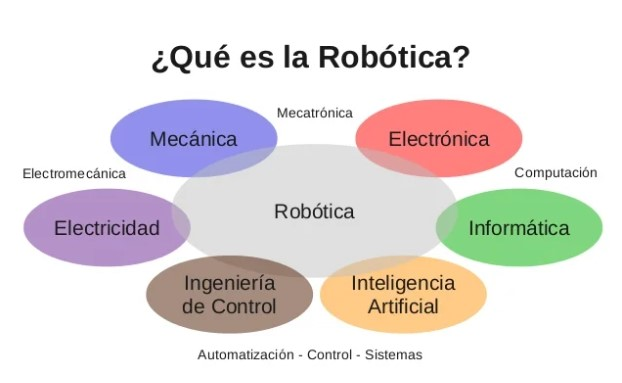
\includegraphics[width=0.7\linewidth]{imagenes/cap1/disciplinas_robotica.jpg} 
    \caption{Disciplinas que componen la robótica.}
    \label{fig:Disciplinas que componen la robótica.} 
\end{figure}

\bigskip

Con los recientes avances en mecatrónica, informática e \ac{IA}, la robótica ha encontrado su lugar en una amplia gama de sectores. En el sector industrial, los brazos robóticos desempeñan roles cruciales en cadenas de montaje, automatizando y refinando diversos procesos. Paralelamente, en el sector doméstico, la robótica ha transformado nuestras rutinas diarias: desde aspiradoras inteligentes que se desplazan con precisión por nuestros hogares, hasta avanzados robots de cocina que simplifican la preparación de alimentos.
\bigskip


\section{Los robots móviles }
\label{sec:Los_robots_móviles}

Los robots, a lo largo de su evolución, han sido clasificados de diversas maneras en función de su diseño, propósito y contexto de aplicación. Los robots humanoides, con su semejanza a la figura humana, buscan emular nuestros movimientos y comportamientos para adaptarse a nuestro mundo. Existen también robots colaborativos que, en lugar de reemplazar a los humanos, están diseñados para trabajar junto a nosotros en entornos compartidos. También podemos distinguir los ya mencionados robots industriales, sin embargo y a pesar de esta diversidad, existe una clasificación que destaca sobre el resto, debido a su gran importancia en la historia de la robótica y a su continuo desarrollo, estos son los robots móviles. Un robot móvil es un sistema robótico que puede desplazarse en distintos entornos y que cuenta con una serie de capacidades que le permiten ejecutar tareas complejas, ya sea de forma autónoma o controlados por un operador humano. \cite{los-robots-móviles}

\bigskip

\begin{figure}[h] 
    \centering
    
\includegraphics[width=0.7\linewidth]{imagenes/cap1/robot_movil.png} 
    \caption{Ilustración de un robot móvil generado por \acs{IA}.}
    \label{fig:Ilustración de un robot móvil generado por IA} 
\end{figure}

\bigskip

A diferencia de los robots fijos, que permanecen estacionarios y realizan tareas desde una posición establecida como por ejemplo los brazos roboticos en una cadena de montaje, los robots móviles \cite{robots-moviles-2} cuentan con la capacidad de desplazarse de un sitio a otro. Esto les otorga una libertad sin precedentes y les permite realizar todo tipo de acciones que para muchas otras máquinas resultan imposibles. Esta versatilidad se debe, en gran parte, a avanzados sistemas de sensores que les permiten percibir su entorno, algoritmos de navegación y control que delinean sus trayectorias; sistemas de comunicación que los conectan con otras máquinas, con bases de datos y teleoperadores e incluso con otros robots. Y a sofisticados actuadores, tales como ruedas, patas, hélices y un largo etcétera, en función de a qué medios deba adaptarse el robot.

\bigskip

En el panorama de la robótica móvil, a pesar de la diversidad y versatilidad de sus aplicaciones, una categoría ha destacado del resto. Los vehículos autónomos son, probablemente, los protagonistas de la robótica móvil del siglo XXI. Estos robots son vehículos equipados con sofisticados sensores que les permiten percibir su entorno, procesar esa información mediante algoritmos avanzados para reaccionar ante él de manera inteligente, imitando el comportamiento de conducción humano. Estos vehículos consiguen esta gran hazaña gracias a una característica muy importante: la conducción autónoma.

\bigskip

\section{La conducción autónoma }
\label{sec:La_conducción_autónoma}

La conducción, en su esencia, se refiere a la acción de guiar o controlar un vehículo, ya sea motorizado o no, con la finalidad de trasladarse de un lugar a otro. Desde tiempos prehistóricos, la humanidad ha tenido la necesidad de trasladarse y transportar bienes, materias primas y otras personas. esta necesidad impulsó la creación de vehículos sencillos como carros tirados por animales o vehículos impulsados por la propia potencia muscular del conductor, como las bicicletas.

\bigskip

Con el paso del tiempo y el avance de la ingeniería y la ciencia en el mundo de la automoción, en el siglo XIX aparecieron los primeros vehículos motorizados. Estos prototipos, movidos inicialmente por vapor y luego por combustibles fósiles, marcaron el inicio de una revolución en la movilidad y transformaron la manera en que las personas y mercancías se desplazaban. Sin embargo, estos vehículos requerían determinadas habilidades manuales y cognitivas por parte del conductor, además de amplios conocimientos de la máquina que se opera. Así, la conducción se convirtió en una habilidad que las personas debían estudiar, practicar y aprender. Adicionalmente, el acto de conducir, para ser ejecutado de manera correcta y segura, requiere de atención, calma y claridad mental, estados que en ocasiones resultan difíciles de mantener para los seres humanos, sobre todo en situaciones desconocidas, inciertas y estresantes, situaciones que son el pan de cada día de cualquier conductor. Todo esto ha hecho que la conducción sea una de las habilidades más difíciles de adquirir y a la vez más valoradas en la actualidad.

\bigskip

Debido a esto, la idea de vehículos que pudieran conducirse por sí mismos, sin necesidad de intervención humana y de las habilidades y atención del conductor, ha sido una aspiración de la humanidad por mucho tiempo, muy probablemente desde el inicio mismo de la conducción. Sin embargo, no fue hasta finales del siglo XX cuando esta idea empezó a parecer viable. Durante este período, la emergencia de la computación, la inteligencia artificial y una amplia gama de sensores avanzados resultaron en vehículos capaces de interpretar su entorno, tomar decisiones y operar sin intervención humana directa en ciertas condiciones estableciendo así el inició de la conducción autónoma. La conducción autónoma se define como la capacidad total o  parcial de que un vehículo pueda conducir autónomamente sin necesidad de un operador externo. \cite{la-conducción-autónoma}

\begin{figure}[h] 
    \centering
    
\includegraphics[width=0.7\linewidth]{imagenes/cap1/conduccion_autonoma.png} 
    \caption{Ilustración de coches autónomos generada por \ac{IA}.}
    \label{Ilustración de coches autónomos generada por IA}
\end{figure}


\newpage



Existen 6 niveles de conducción autónoma según el estándar establecido por la \ac{SAE} en el estándar J3016 \cite{estándar-j3016}

\begin{enumerate}
        \item \textbf{Nivel 0 (No Automation)}:
         El conductor humano es responsable de todas las tareas de conducción, incluso si el vehículo ofrece alguna intervención momentánea.
        \bigskip

    \item \textbf{Nivel 1 (Driver Assistance)}:

        El vehículo puede asistir al conductor en una única tarea de conducción (por ejemplo, control de crucero).
        El conductor sigue siendo responsable de la mayoría de las tareas y debe estar atento en todo momento.
       \bigskip

    \item \textbf{Nivel 2 (Partial Automation)}:

         El vehículo puede controlar simultáneamente dos tareas, como dirección y aceleración.
         A pesar de esta automatización, el conductor debe supervisar el sistema en todo momento.
       \bigskip

    \item \textbf{Nivel 3 (Conditional Automation)}:

         El vehículo puede realizar la mayoría de las tareas de conducción en ciertas condiciones, pero requerirá intervención humana cuando el sistema lo solicite.
         El conductor debe estar disponible para tomar el control, pero no necesita tener las manos en el volante todo el tiempo.
       \bigskip

    \item \textbf{Nivel 4 (High Automation)}:

        En ciertos escenarios o zonas geográficas específicas, el vehículo puede manejar todas las tareas de conducción.
        Fuera de estas zonas, el vehículo podría requerir que el conductor tome el control.
      \bigskip

    \item \textbf{Nivel 5 (Full Automation)}:

        El vehículo es completamente autónomo en todos los escenarios y condiciones.
        No necesita un volante, pedales ni un conductor humano.
      \bigskip
\end{enumerate}

\newpage

\begin{figure}[h] 
    \centering
    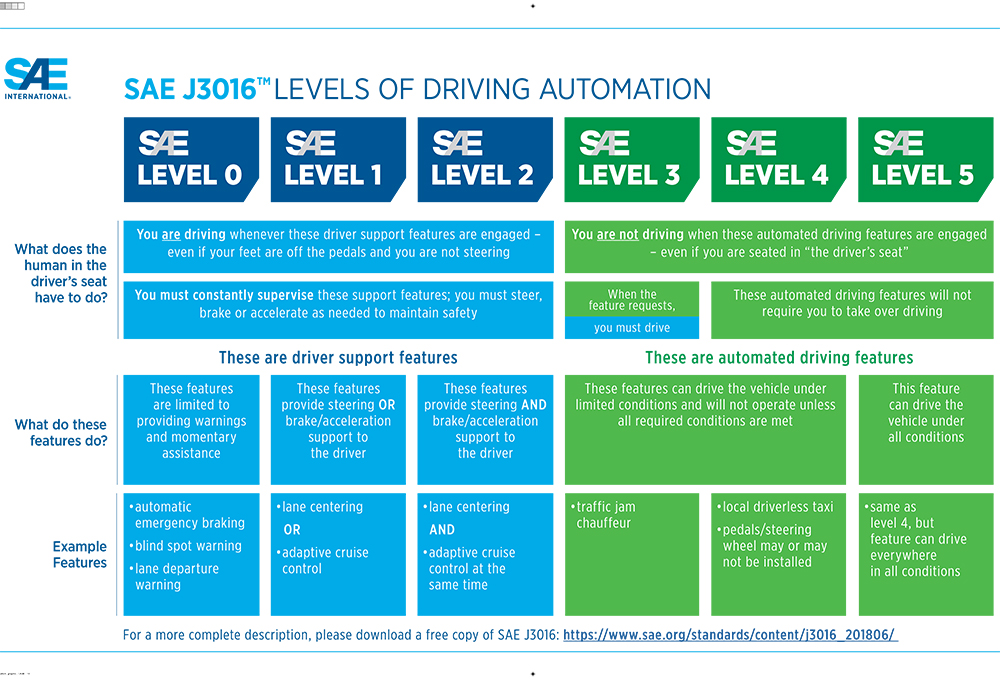
\includegraphics[width=1\linewidth]{imagenes/cap1/niveles_conduccion_autonoma.jpg} 
    \caption{Niveles de conducción autónoma según el estándar J3016}
    \label{fig:Niveles de conducción autónoma según el estándar J3016} 
\end{figure}

\bigskip

El final del siglo XX y el comienzo del siglo XXI marcaron una era significativa en el avance de la conducción autónoma. Los primeros sistemas y algoritmos para la conducción autónoma derivaban de los \ac{ADAS}. Según la página oficial de la DGT \cite{ADAS_DGT} estos sistemas representan un conjunto de tecnologías integradas en vehículos que no solo mejoran la seguridad sino también la experiencia del conductor. Operan con diferentes grados de autonomía y pueden influir en múltiples funciones del vehículo, como frenado, aceleración, dirección y señalización. Sistemas como el \ac{ISA}, que regula constantemente la velocidad del vehículo; el \ac{REV}, que alerta sobre obstáculos al retroceder; y el \ac{LKA}, que asegura que el vehículo permanezca dentro de un carril, sitúan a los coches que los incorporan dentro de los primeros 2 niveles de autonomía \cite{articulo-academico-tesla}. No obstante, con el auge de la \ac{IA}, la emergencia de las redes neuronales y los avances en computación, los sistemas \ac{ADAS} han evolucionado con rapidez. Este progreso ha permitido a empresas como Tesla desarrollar los primeros vehículos comerciales de nivel 2. En cuanto a los niveles de autonomía más avanzados tenemos a compañías como Waymo, quien como se explica en ese artículo académico \cite{tesla_y_robotaxi} esta embarcado en un proyecto para crear una flota de taxis autónomos.

\newpage

\begin{figure}[h] 
    \centering
    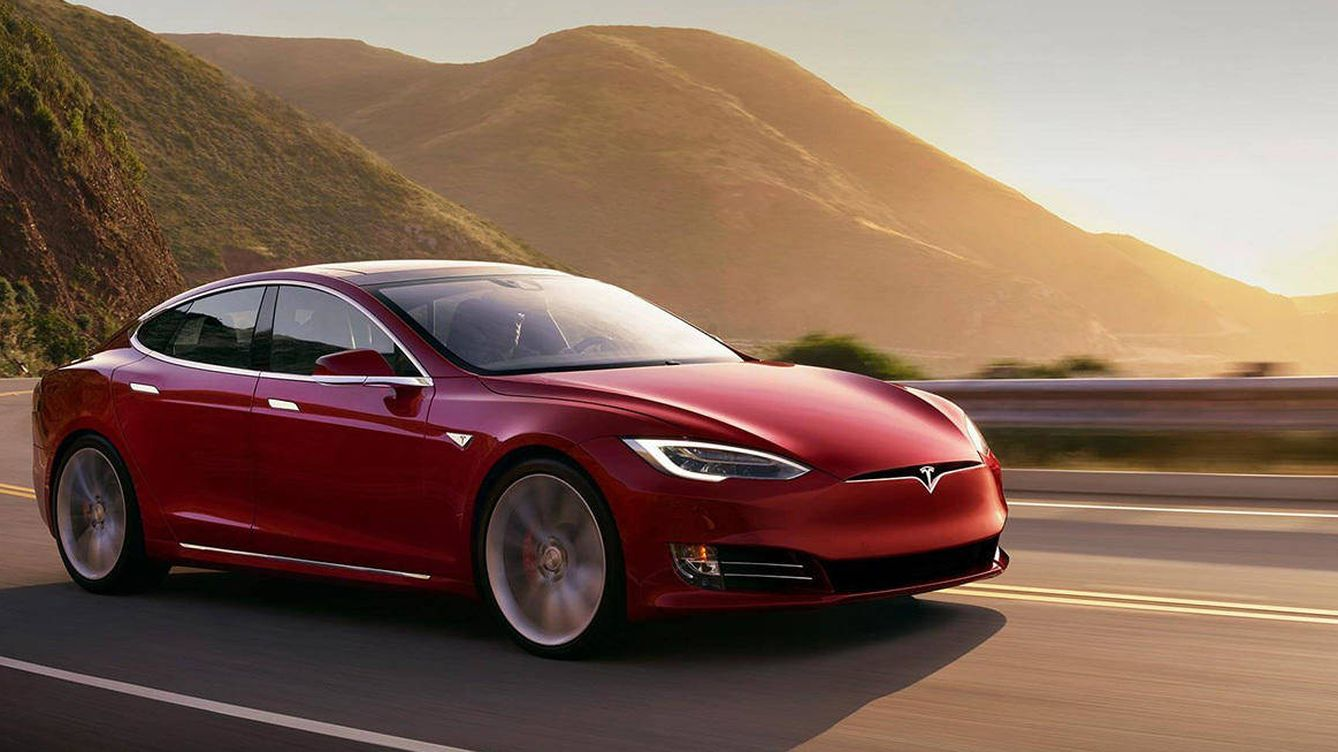
\includegraphics[width=0.7\linewidth]{imagenes/cap1/tesla.jpg} 
    \caption{Vehículo tesla}
    \label{fig:Vehículo tesla} 
\end{figure}


\bigskip

Los llamados robotaxis  \cite{robotaxi} , son actualmente una serie de taxis de nivel de autonomía 4 que operan en algunas ciudades de Estados Unidos. Estos vehículos están pensados para transportar pasajeros de manera completamente autónoma, sin la necesidad de un conductor humano, de hecho estos taxis futuristas no incluyen pedales ni volante como se puede observar en la figura \ref{fig:robotaxi}. Los robotaxi actualmente realizan viajes con pasajeros reales seleccionados en algunas zonas de Phoenix y San Francisco con el fin de recopilar datos y en general probar y madurar esta nueva tecnología para así en un futuro próximo convertir los robotaxis en un producto comercial que revolucione el transporte en las ciudades

\bigskip

\begin{figure}[h] 
    \centering
    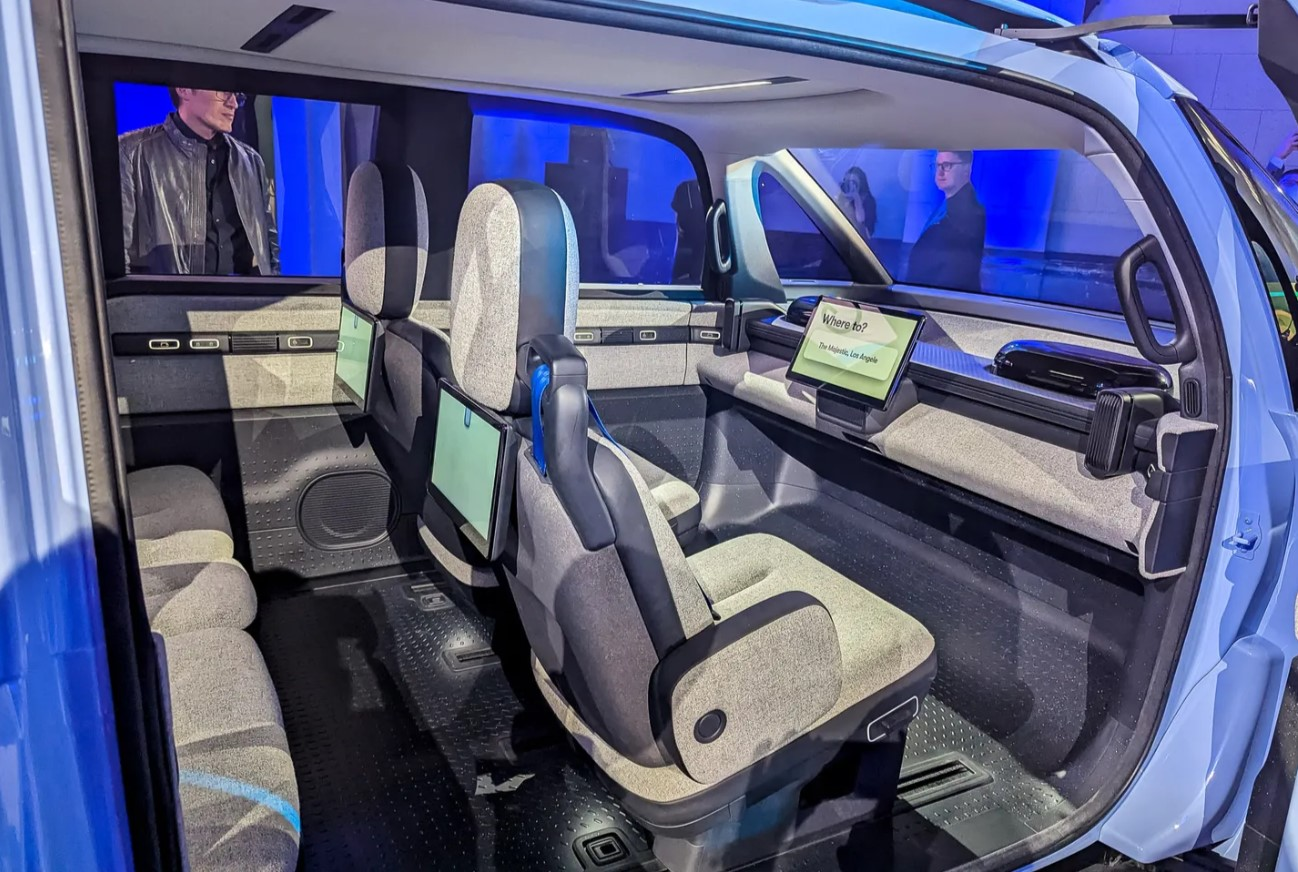
\includegraphics[width=0.7\linewidth]{imagenes/cap1/waymo_robotaxi.jpg} 
    \caption{Interior de un robotaxi de Waymo}
    \label{fig:robotaxi}
\end{figure}


\newpage

Sin embargo, a pesar de todos los avances de los últimos años en el ámbito de la conducción autónoma, esta problemática sigue sin estar completamente solucionada y los vehículos de nivel 4 y 5 de autonomía todavía son solo prototipos y no productos comerciales certificados y testados como podemos leer en este \ac{TFM} \cite{estado_del_arte_conducción_autónoma}. Esto se debe a que la conducción autónoma es una de las áreas más desafiantes dentro de la ingeniería y la robótica, dada la inmensa complejidad y variabilidad de los escenarios en los que estos vehículos deben operar. Estos entornos no son estáticos, sino que están en constante cambio y movimiento. Carreteras en constante transformación, condiciones meteorológicas cambiantes, variaciones de luz, obstáculos inesperados y una amplia variedad de usuarios de la vía, desde peatones hasta ciclistas y otros vehículos, hacen que la carretera sea uno de los entornos más impredecibles. Añadiendo una capa adicional de complejidad, se encuentra el factor humano. No solo los vehículos autónomos deben anticipar y responder a las acciones de los conductores humanos, que pueden ser a menudo ilógicas o imprevistas, sino que además deben garantizar la máxima seguridad para los peatones y otros usuarios de la vía. Convivir en un espacio compartido con seres humanos requiere de un cuidado y precisión extraordinarios, pues el más mínimo error podría tener consecuencias extremadamente graves como se menciona en este artículo académico en la revista Nature \cite{peligros_conducción_autónoma}

\bigskip

No obstante, una conducción autónoma perfecta promete revolucionar radicalmente el paradigma de movilidad y seguridad en nuestras carreteras tal y como explica este artículo publicado en la revista ScienceDirect \cite{la_revolución_de_la_conducción_autónoma}. La mayoría de los accidentes en la carretera son causados por errores humanos, ya sea por distracción, fatiga o decisiones erróneas en situaciones críticas. Los vehículos autónomos, operando con una combinación de sensores avanzados y algoritmos sofisticados, tienen el potencial de minimizar estos errores, reaccionando más rápidamente y de manera más precisa que un humano ante situaciones imprevistas. Además, los sistemas de conducción autónoma podrían gestionar de forma más eficiente el flujo de tráfico. Al poder comunicarse entre sí, los vehículos podrían coordinarse para evitar atascos, optimizar el uso de carriles y reducir las congestiones, resultando en viajes más rápidos y eficientes para todos. Por último, pero no menos importante, liberar a los humanos de la tarea de conducir abre un mundo de posibilidades. Las personas podríamos ocupar todo el tiempo que dedicamos hoy en día a la conducción en otras acciones más provechosas o entretenidas: leer, ver una película, trabajar o incluso descansar. Esto mejoraría la calidad de vida al proporcionar tiempo adicional para actividades personales o productivas. En definitiva, las ventajas que nos presenta la conducción autónoma son múltiples y muy interesantes; es una tecnología que, sin duda, cambiará el mundo.

\section{La inteligencia artificial en la conducción autónoma}
\label{sec:La inteligencia artificial en la conducción autónoma}

La \ac{IA} ha desempeñado un papel fundamental en la evolución de la conducción autónoma, permitiendo que los vehículos interpreten su entorno, tomen decisiones y se adapten a situaciones cambiantes. Al principio, la \ac{IA} en la conducción autónoma se basaba en algoritmos más básicos basados en visión artificial y procesamiento de imágenes. Sin embargo, pronto se hizo evidente que para alcanzar los niveles más altos de autonomía era necesario un enfoque más sofisticado para gestionar la complejidad. Esto condujo a la adopción y desarrollo de técnicas más avanzadas.

\textbf{Las redes neuronales} se han convertido en herramientas esenciales en el campo de la conducción autónoma \cite{Implementación_de_redes_neuronales_para_conducción_autónoma}. Estas redes, que imitan la estructura y el funcionamiento de las neuronas humanas, son particularmente aptas para tareas como la detección y la identificación de objetos. Al ser entrenadas con grandes cantidades de datos, pueden reconocer patrones y categorizar objetos en tiempo real con una precisión impresionante como se muestra en el siguiente \ac{TFG} de un estudiante de la universidad de \ac{ULPGC} \cite{detección_de_objetos_con_redes_neuronales}

\textbf{El imitation learning}, o aprendizaje por imitación \cite{imitation-learning-2}, es una técnica que permite a los sistemas de \ac{IA} aprender a partir de la observación directa de acciones realizadas por humanos u otros agentes. En el contexto de la conducción autónoma, se puede utilizar para enseñar a los vehículos a imitar las decisiones y acciones de conductores humanos experimentados en diversas situaciones, permitiendo que los vehículos aprendan comportamientos más naturales. En el \ac{TFM} que a continuación se cita se explora una solución para la conducción autónoma basada en imitation learning \cite{conducción_autónoma_imitation_learning}.

\textbf{El aprendizaje por refuerzo} es otra técnica de \ac{IA} crucial en la conducción autónoma. Este método entrena modelos de \ac{IA} a través de recompensas y penalizaciones, permitiéndoles aprender a tomar decisiones óptimas en situaciones específicas \cite{RL-2}. Por ejemplo, un vehículo autónomo podría ser recompensado por evitar obstáculos y penalizado por acercarse demasiado a ellos, aprendiendo con el tiempo a navegar de manera más segura y eficiente. En la documentación de continuación se puede encontrar información más detallada sobre el aprendizaje por refuerzo \cite{aprendizaje_por_refuerzo}

\newpage

\begin{figure}[h]
	\centering
	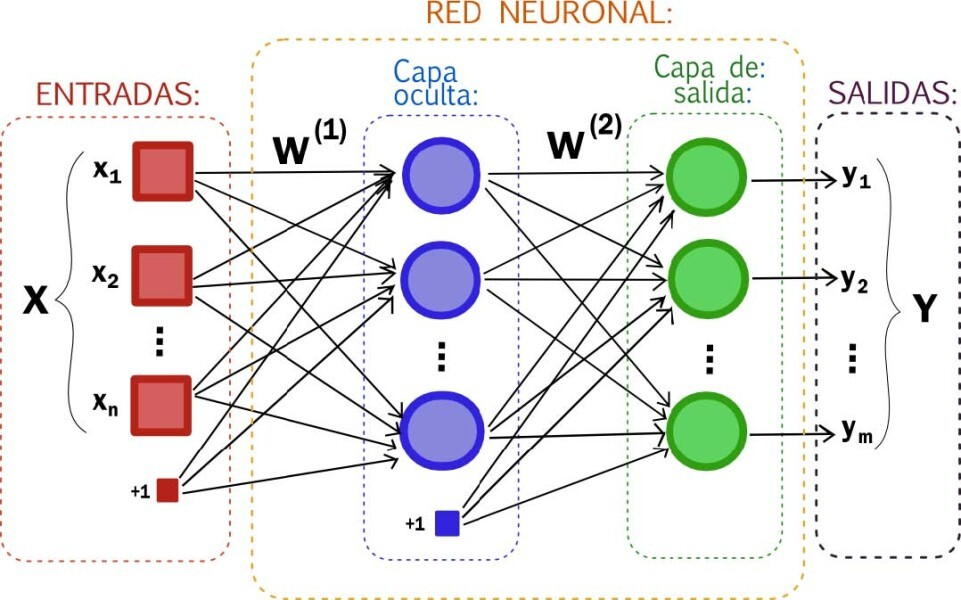
\includegraphics[width=0.7\linewidth]{imagenes/cap1/red_neuronal.jpeg}
	\caption{Ilustración de una red neuronal}
	\label{fig:Ilustración de una red neuronal}
\end{figure}

En resumen, la inteligencia artificial ha revolucionado significativamente el ámbito de la conducción autónoma. Las principales empresas tecnológicas y automotrices, como Waymo, Tesla y Cruise, han desarrollado y probado vehículos con niveles avanzados de autonomía, principalmente en niveles 2 y 3 e incluso en algunos casos con capacidades limitadas de nivel 4 en entornos específicos. A pesar de los logros técnicos, la complejidad que representa navegar por nuestras carreteras sitúa aún lejos vehículos capaces de alcanzar niveles 4 y 5 completos de autonomía \cite{Niveles-altos-autonomía}.

\section{ Conducción autónoma en CARLA con adaptación al tráfico basado en aprendizaje por refuerzo}
\label{sec:Conducción autónoma en CARLA basada en aprendizaje por refuerzo con adaptación al tráfico}

El \ac{TFG} que a continuación se presenta aborda una investigación académica sobre la conducción autónoma basada en aprendizaje por refuerzo. Se pretende solucionar varias problemáticas relacionadas con el seguimiento de carril con un vehículo autónomo de manera fluida y segura. Por otro lado, aparte de esta hazaña este \ac{TFG} pretende llegar un paso mas allá diseñando sistemas de seguimiento de carril con funciones añadidas como la capacidad de frenar para evitar la colisión frontal con obstáculos y adaptarse al tráfico presente en la vía de manera fluida.

\bigskip




  

\chapter{Objetivos}
\label{cap:capitulo2}

En el capítulo \ref{cap:capitulo1}, se ha descrito e introducido el contexto en el que se enmarca este \ac{TFG}. En este segundo capítulo, que a continuación se expone, se procederá a presentar los objetivos específicos que se han establecido para este proyecto.

\section{Descripción del problema}
\label{sec:descripcion_problema}

Como se menciona en el primer capítulo, la conducción autónoma promete ser un avance tecnológico que cambie completamente la manera en la que se concibe la movilidad en nuestra sociedad. Este trabajo de fin de grado tiene como principal objetivo realizar una investigación sobre la utilización de distintas técnicas de \ac{IA}, para la creación de una solución completa para la problemática de la navegación por un carril. Se presentará un comportamiento dotado de la capacidad de seguir un carril, adaptarse al tráfico de este y evitar colisiones en caso de que el tráfico se detenga.

\section{Objetivos}
\label{sec:Objetivos}

\begin{enumerate}
	\item Instalación y configuración del simulador CARLA, ROS 2, logrando además una comunicación entre ambos.
	\item Análisis de la viabilidad de desarrollar aplicaciones de conducción autónoma mediante el uso del simulador foto-realista CARLA y el framework de aplicaciones roboticas ROS 2, utilizando \textit{CARLA to ros bridge} como medio de comunicación.
	\item Creación de un comportamiento sigue carril autónomo basado en aprendizaje por refuerzo.
	\item Desarrollar un comportamiento para, además de navegar por un carril de manera segura, detenerse antes de colisionar con obstáculos de la carretera.
	\item Elaboración de un comportamiento que permita a un vehículo adaptarse a la velocidad del tráfico a la hora de navegarautonomamente  por un carril utilizando aprendizaje por refuerzo.
	\item Análisis de métricas de los algoritmos desarrollados en el \ac{TFG} y realización de una comparativa entre estas métricas.
\end{enumerate} 


\section{Requisitos}
\label{sec:requisitos}

Los requisitos que ha de cumplir este trabajo son los siguientes:
\begin{itemize}
	\item El trabajo ha de realizarse en el simulador foto-realista de conducción autónoma CARLA.
	\item Los sistemas a desarrollar deben ser reactivos, es decir deben ser capaces de reaccionar a su entorno de manera rápida y precisa.
	\item El vehículo debe navegar de manera adecuada, natural y segura.
\end{itemize}

\section{Metodología}
\label{sec:metodologia}

El \ac{TFG} comenzó en octubre de 2022 y finalizó también en octubre de 2023. A lo largo de estos 12 meses se siguieron las siguientes directrices para la realización del mismo:
\begin{itemize}
	\item Reuniones semanales el tutor del \acs{TFG} para establecer micro-objetivos semanales y reales. Gracias a estas reuniones, fue fácil mantener un control del avance del proyecto en cada momento e ir solucionando de manera rápida y efectiva los problemas que surgían.
	\item Realización de un blog\footnote{\url{https://roboticslaburjc.github.io/2022-tfg-juancamilo-carmona/}}. en el que se añadían periódicamente entradas con información sobre el avance del proyecto, además de los problemas enfrentados en cada etapa, a modo de bitácora para documentar todo el proceso de desarrollo.
	\item Se utilizó la plataforma de comunicación Microsoft Teams para realizar las reuniones periódicas con mi tutor del TFG y el correo de la universidad para mantener contacto con él en todo momento, con el fin de resolver problemas que pudieran surgir, notificar avances y solicitar consejos.
	\item Se empleó la plataforma de desarrollo GitHub para alojar todo el código desarrollado en el \ac{TFG} \footnote{\url{https://github.com/RoboticsLabURJC/2022-tfg-juancamilo-carmona}}.
	\item En el desarrollo de este \ac{TFG}, se adoptó la metodología Scrum como sistema de trabajo. A lo largo del desarrollo de este trabajo, se establecieron diferentes sprints, cada uno de ellos con una duración determinada, durante los cuales se plantearon mini objetivos específicos a alcanzar. Esta estructura no solo permitió una organización y planificación eficiente del trabajo, sino que también ofreció la flexibilidad necesaria para adaptarse a cambios y nuevos requerimientos que surgieron a lo largo del desarrollo del \ac{TFG}.
	
\begin{figure}[h]
	\centering
	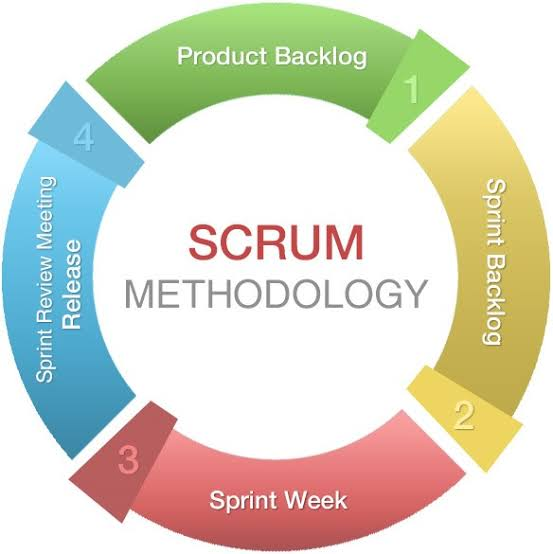
\includegraphics[width=0.5\linewidth]{imagenes/cap2/scrum.jpg}
	\caption{Ilustración de la metodología scrum}
	\label{fig:Ilustración de la metodología scrum}
\end{figure}
\end{itemize}

\section{Plan de trabajo}
\label{sec:plantrabajo}

Durante los 12 meses en los que se ha desarrollado este proyecto, se ha seguido un plan de trabajo con la siguiente estructura:
\begin{enumerate}
	\item Etapa de configuración: Esta etapa consistió básicamente en preparar todo el entorno para la realización del \ac{TFG}. Aquí se instalaron todos los drivers, software y aplicaciones necesarias para empezar a trabajar.
	\item Comienzo del \ac{TFG}: Una vez el entorno de trabajo estaba listo, se empezó a desarrollar todo el código.
	\begin{itemize}
		\item En primer lugar, se inició con el desarrollo de un teleoperador para un vehículo.
		\item En segunda instancia, una vez el teleoperador estaba terminado, se continuó con los algoritmos de seguimiento de carril con percepción basada visión artificial tradicional y un algoritmo con percepción basada en una red neuronal.
		\item Una vez finalizado el desarrollo de los algoritmos de percepción, la siguiente etapa consistió en analizar las métricas de todos ellos y compararlas para llegar a una conclusión sobre la mejor solución para la problemática.
		\item El siguiente paso, fue programar un sigue carril basado en aprendizaje por refuerzo.
		\item Una vez terminado el comportamiento sigue carril, se procedió a añadir un comportamiento el cual permitiera no chocarse al encontrar obstáculos en la carretera.
		\item Finalmente se trabajó en una solución más completa de conducción autónoma que navegara por un carril correctamente, deteniéndose en caso de encontrar un vehículo u obstáculo detenido y adaptándose a la velocidad del tráfico sin colisionar ni ni detener la marcha en caso de que este existiera.
	\end{itemize}
	\item Para finalizar, se procedió a la redacción de la memoria del \ac{TFG}.
\end{enumerate}



\chapter{Plataformas de desarrollo y herramientas utilizadas}
\label{cap:capitulo3}

En el capitulo que a continuación se presenta se van a describir las distintas plataformas y herramientas que se han utilizado a lo largo desarollo de este \ac{TFG}

\section{Lenguajes de programación}
\label{sec:lenguajes_programacion}

\subsection{Python}
\label{subsec:python}

Python es un lenguaje de programación orientado a objetos, de alto nivel y fácil de interpretar, con una sintaxis sencilla y legible \cite{que_es_python_1}. Actualmente, es uno de los lenguajes de programación más populares y resulta especialmente útil para el desarrollo de prototipos. Esto se debe a su facilidad de uso, que permite codificar algoritmos complejos de manera rápida y ágil. Además, es muy utilizado para desarrollar aplicaciones y algoritmos de inteligencia artificial, gracias a la gran cantidad de bibliotecas especializadas que este lenguaje ofrece \cite{python_y_la_ia}. Todo el código desarrollado para este \ac{TFG} ha sido realizado íntegramente en Python, lo cual ha facilitado enormemente tanto la fase de investigación como la de implementación, permitiéndonos centrarnos más en la lógica de los algoritmos y menos en las complicaciones del lenguaje en sí. Esta elección ha demostrado ser acertada y ha contribuido significativamente al éxito del proyecto. 

\begin{code}[H]
\begin{lstlisting}[language=Python
]
 def accelerate(self):
    control = VehicleControl()  
    control.throttle = 0.5
    self.vehicle.apply_control(control)      
    
\end{lstlisting}
\caption[Ejemplo de código Python]{Ejemplo de código Python}
\label{cod:holamundo_python}
\end{code}

\newpage

\section{Entornos de programación}
\label{sec:entornos_de_programacion}


\subsection{CARLA}
\label{subsec:CARLA}

Dentro del extenso panorama de simuladores dedicados a la conducción autónoma, encontramos un sinfín de opciones. Sin embargo, entre toda esta variedad de simuladores, CARLA destaca como una de las herramientas más interesantes. CARLA es un simulador de conducción autónoma realista de código abierto que ha ganado prominencia en la comunidad de investigación y desarroll, su alto grado de foto-realismo, el amplio control que ofrece sobre el entorno simulado y la gran cantidad de vehículos y sensores disponibles la convierten en una de las mejores elecciones a la hora de desarrollar y probar todo tipo de proyectos relacionados con la conducción autónoma. Fue creado por el equipo del Computer Vision Center en Barcelona en colaboración con Intel Labs y Toyota Research Institute. Desde su lanzamiento en 2017, CARLA ha sido una de las herramientas más prometedoras del mundo de la conducción autónoma.

\bigskip 

La principal y más importante fortaleza de este simulador probablemente sea su nivel de foto-realismo. CARLA ofrece un alto nivel de detalle y precisión en sus simulaciones, que garantiza que los desarrolladores puedan probar algoritmos en condiciones que emulan fielmente situaciones del mundo real, como cambios de luz y de sombras, choques y colisiones, situaciones de altas y bajas velocidades, entre muchas otras características que sitúan a este simulador un paso por delante en cuanto a este aspecto se refiere se refiere.

\bigskip

Otra de las fortalezas más destacables de CARLA es su elevado número de escenarios. Estos abarcan desde entornos urbanos, como calles de barrios, rotondas, etc., hasta entornos interurbanos como autopistas y carreteras convencionales e incluso entornos rurales como granjas. Esto nos permite a los ingenieros y desarrolladores simular innumerables contextos y situaciones de conducción. Adicionalmente, CARLA brinda gran control sobre las condiciones ambientales. Los usuarios tienen la ventaja de ajustar aspectos tan vitales como la luminosidad, hora del día y condiciones climáticas, creando un espacio flexible y diverso para pruebas y experimentos especialmente aquellos relacionados con la \ac{IA}.

\bigskip

La diversidad de activos probablemente sea la última de las fortalezas de CARLA. Su biblioteca contiene una amplia gama de vehículos, peatones y sensores, abarcando desde cámaras RGB hasta sistemas LIDAR, radares y electro-ópticos, ofreciendo así una rica paleta de herramientas para las simulaciones.

\bigskip

\begin{figure} [H]
	\begin{center}
	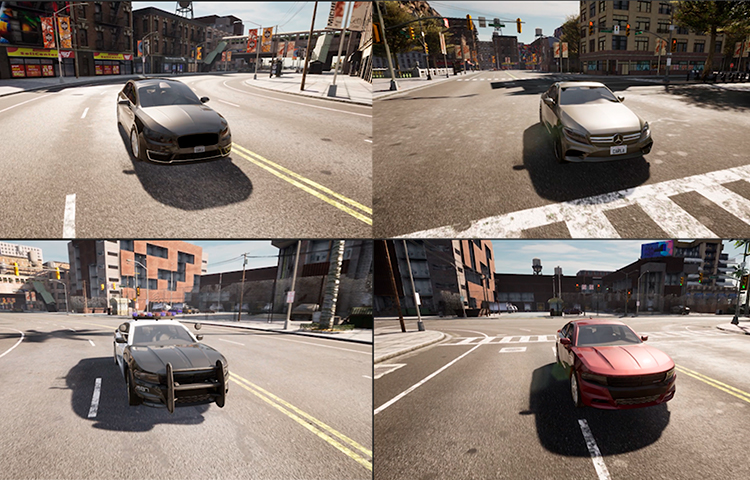
\includegraphics[height=8cm]{imagenes/cap3/carla.jpg}
	\end{center}
	\caption[Imagén de vehículos en CARLA]{Imagén de vehículos en CARLA}
	\label{fig:CARLA_vehicles}
\end{figure}

CARLA es una de las piezas clave de este \ac{TFG} es el escenario virtual en el que se desarrollan, prueban y evalúan todos los algoritmos y modelos diseñados para las problemáticas de conducción autónoma planteadas. \footnote{\url{https://carla.org/}}


\subsection{ROS 2}
\label{subsec:Ros 2}

ROS 2, la evolución de segunda generación de ROS, es un meta sistema operativo de código abierto diseñado específicamente para ser utilizado en robots. Proporciona servicios que se esperarían de un sistema operativo, incluyendo abstracción de hardware, control de dispositivos de bajo nivel e implementación de funcionalidades \cite{introducción_a_ros}. Una de las características fundamentales de ROS es su modelo de comunicación basado en el sistema publicador-suscriptor. En este sistema, los nodos (componentes individuales de software en un sistema ROS y ROS 2) pueden comunicarse entre sí de manera asíncrona. Un nodo que tiene información para compartir se convierte en un publicador y envía mensajes a un topic. Otros nodos que estén interesados en recibir esa información se suscriben a ese y recibirán los mensajes publicados en él. Esto permite una comunicación eficiente y flexible entre los diferentes nodos que conformen nuestro sistema.

\bigskip
\begin{figure} [H]
	\begin{center}
	
\includegraphics[height=3cm]{imagenes/cap3/ros2_logo.png}
	\end{center}
	\caption[logotipo de Ros 2]{Logotipo de Ros 2}
	\label{fig:Ros2_logos}
\end{figure}
\bigskip

En el desarrollo de este Trabajo de Fin de Grado, ROS 2 se utilizó para elaborar una sección específica del código y de los algoritmos de conducción autónoma. La decisión de integrar ROS 2 con el simulador CARLA tuvo un propósito muy claro: evaluar la viabilidad de unir las capacidades de este sistema, que es una referencia en el mundo de la robótica, con el entorno de simulación de conducción autónoma que CARLA ofrece. Esta integración se realizó con el objetivo de no solo generar algoritmos más robustos y eficaces sino también de explorar nuevas posibilidades y métodos para la creación de sistemas de conducción autónoma. Esta fusión entre ROS 2 y CARLA se convirtió en un elemento clave para entender y desarrollar más a fondo los complejos retos que plantea la conducción autónoma, permitiendo una interacción más fluida y adaptable entre los diferentes componentes del sistema. \footnote{\url{https://www.ros.org/}}

\bigskip 

\subsection{CARLA to ros bridge}
\label{subsec:CARLA to ros bridge}

\textit{CARLA to ros bridge} es una herramienta oficial desarrollada por el equipo de CARLA. Esta herramienta tiene el objetivo de ser,  un medio de comunicación bidireccional entre CARLA y un entorno de desarrollo ROS o ROS2. Por un lado el bridge de encarga de traducir la información de CARLA  a topics y mensajes de ROS de manera que el framework  pueda entenderlos sin mayor dificultad. Por otro lado el bridge se encarga también de traducir los mensajes publicados en los topics generados para CARLA en mensajes basados en la\ac{API} del simulador para que, de esta manera un nodo ROS 2 pueda comunicarse con CARLA como lo haría con cualquier robot. carla to ros bridge puede ser encontrado de su repositorio oficial de Github, en el aparte del código encontraremos instrucciones para su descarga y uso\footnote{\url{https://github.com/carla-simulator/ros-bridge}}
\begin{figure} [H]
	\begin{center}
	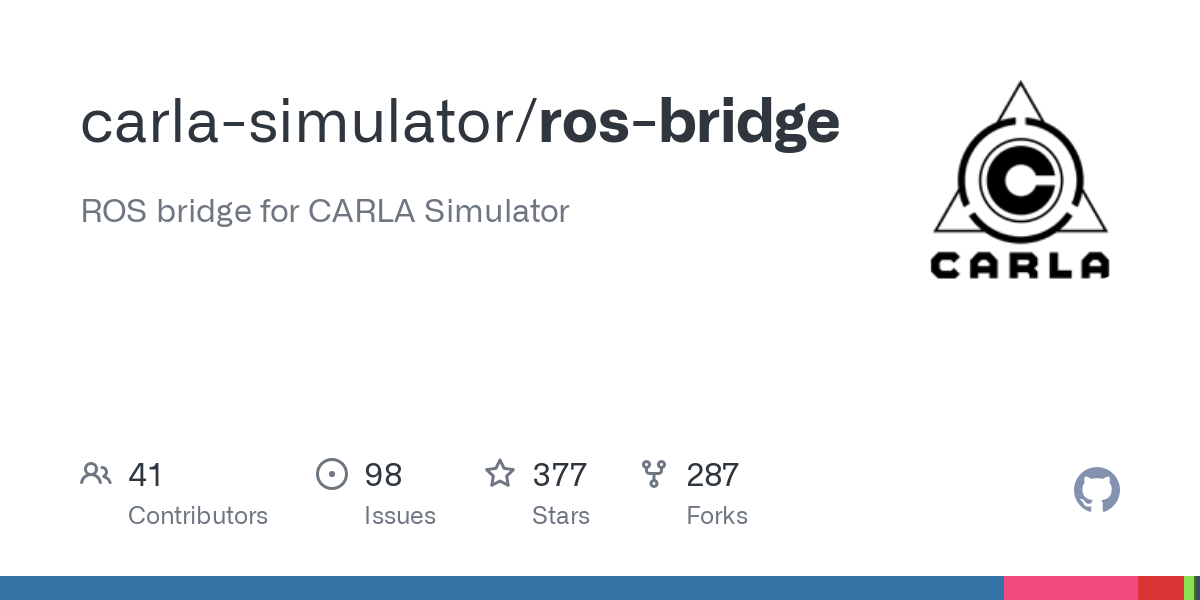
\includegraphics[height=6cm]{imagenes/cap3/carla_to_ros_bridge.png}
	\end{center}
	\caption[CARLA to ros bridge]{CARLA to ROS bridge}
	\label{fig:carla_to_ros_bridge}
\end{figure}
en este este \ac{TFG} carla to ros bridge ha tenido un papel fundamental  en la fase de investigación y experimentación sobre la viabilidad del desarrollo de algoritmos de conducción autónoma en ROS 2 para el simulador CARLA, permitiendo que CARLA y ROS 2 se comunicarán.


\subsection{Visual studio code}
\label{subsec:Visual studio code}

Visual studio code  \footnote{\url{https://code.visualstudio.com/}} es un editor de código gratis, ligero, profesional y fácil de usar disponible tanto para Linux, como para Windows, como para macOS. Probablemente representa la elección favorita de la gran mayoría de los programadores de hoy en día a la hora de eligir un editor de código. Tanto en ambientes de investigación como en entorno profesionales de producción de aplicaciones y programas Visual studio code es ampliamente conocido y utilizado.

\begin{figure} [H]
	\begin{center}
	
\includegraphics[height=4cm]{imagenes/cap3/vsc-logo.png}
	\end{center}
	\caption[carla to ros bridge]{Visual studio code logo}
	\label{fig:vcs logo}
\end{figure}

Visual studio code ha sido el editor elegido para la programación de todo el código de este \ac{TFG}. Los algoritmos, herramientas y aplicaciones que más tarde se explicarán han sido todas gestados en este famoso editor.

\subsection{PyTorch}
\label{subsec:PyTorch}

PyTorch \footnote{\url{https://pytorch.org/}} es una biblioteca de aprendizaje automático de código abierto desarrollada principalmente por el equipo de inteligencia artificial de Facebook. Es especialmente popular en la comunidad académica y de investigación por su flexibilidad y eficiencia. Compatible con sistemas operativos como Linux, Windows y macOS, PyTorch facilita tanto la investigación experimental como la implementación de modelos en producción. Su diseño intuitivo y las capacidades para realizar cálculos de tensores de manera eficiente lo convierten en una de las bibliotecas más utilizadas en aprendizaje profundo y visión por computadora. En entornos tanto académicos como profesionales, PyTorch es ampliamente reconocido y empleado para una variedad de aplicaciones que van desde el análisis de datos hasta el reconocimiento de imágenes y la robótica. Dentro del contexto de este \ac{TFG} Pytorch se utilizará para cargar y utilizar modelos de redes neuronales en algunas de las implementaciones

\subsection{OpenCV}
\label{subsec:OpenCV}

OpenCV \footnote{\url{https://opencv.org/}} es una biblioteca de visión por computadora de código abierto. Originalmente desarrollada por Intel, OpenCV es especialmente potente para tareas relacionadas con el procesamiento de imágenes, detección de objetos y funciones de realidad aumentada. Es una de las herramientas más utilizadas en el campo de la visión artificial debido a su accesibilidad, eficiencia y comunidad activa. Su amplio conjunto de funciones y utilidades lo hacen versátil y altamente funcional para una variedad de aplicaciones prácticas, desde sistemas de vigilancia y diagnóstico médico hasta vehículos autónomos. En este proyecto Opencv se utilizará como la biblioteca estándar para realizar todo el procesamiento de imágenes necesario para la implementación de los algoritmos y funcionalidades.


\subsection{Pygame}
\label{subsec:Pygame}

Pygame \footnote{\url{https://www.pygame.org/}} Según su página de Wikipedia oficial \cite{pygame}, Pygame es una biblioteca de Python que se utiliza para el desarrollo de videojuegos y aplicaciones multimedia interactivas. Es compatible con sistemas operativos como Linux, Windows y macOS, y su diseño sencillo y la amplia documentación disponible lo convierten en una de las bibliotecas más accesibles para empezar en el mundo del desarrollo de videojuegos. En entornos tanto educativos como de desarrollo indie, Pygame es ampliamente reconocido y utilizado para una variedad de proyectos, en el contexto de este \ac{TFG}, Pygame se utilizará para la implementación de las interfaces gráficas de todas las aplicaciones presentadas

\subsection{Servidor Landau de la Escuela de ingeniería superior de Fuenlabrada de la URJC}
\label{subsec:Servidor landau de la URJC}

Una de las principales limitaciones que los ingenieros nos encontramos a la hora de trabajar con \ac{IA}, es si duda, la necesidad de un hardware potente para el correcto funcionamiento de esta. La ejecución y entrenamiento de algoritmos de inteligencia artificial y aprendizaje automático suelen ser computacionalmente muy pesado lo cuál dificulta su ejecución de manera correcta y fluida sin el Hardware adecuado. Generalmente lo más importante en este aspecto es una \ac{GPU} potente. En el caso del \ac{TFG} que en esta memoria se presenta, existe el problema añadido de que como anteriormente se ha mencionado se utiliza el simulador foto-realista CARLA el cuál por otra parte también requiere un gran cantidad de memoria de \ac{GPU} para poder funcionar. Éstos dos factores hicieron que para realizar este \ac{TFG} fuera vital disponer de una \ac{GPU} muy potente capaz de correr CARLA y a la vez ser capaz de ejecutar algoritmos pesados de \ac{IA}.

\bigskip

Esta problemática hubiera sido probablemente uno de los problemas más grandes a los que este \ac{TFG} se hubiera tenido que afrontar, debido a que el hardware que se necesitaba era sumamente costoso y probablemente inasumible. Afortunadamente esto no fue así ya que la Escuela de ingeniería superior de la \ac{URJC} se ofreció a proporcionar el hardware necesario ofreciendo acceso a un servidor propio y privado de la Universidad el cuál permitía ejecutar código en racks de gráficas Nvidia alojadas en la misma universidad.

\bigskip

El servidor Landau de la Escuela de ingeniería superior de Fuenlabrada, perteneciente a la \ac{URJC} cuenta con 4 gráficas Nvidia A100 de 80 GB cada una. En la figura \ref{fig:graficas servidor landau} se puede ver la información de los recursos gráficos del servidor Landau obtenida del propio servidor mediante la ejecucióin del comando \textit{nvidia-smi}
\bigskip

\begin{figure} [H]
	\begin{center}
	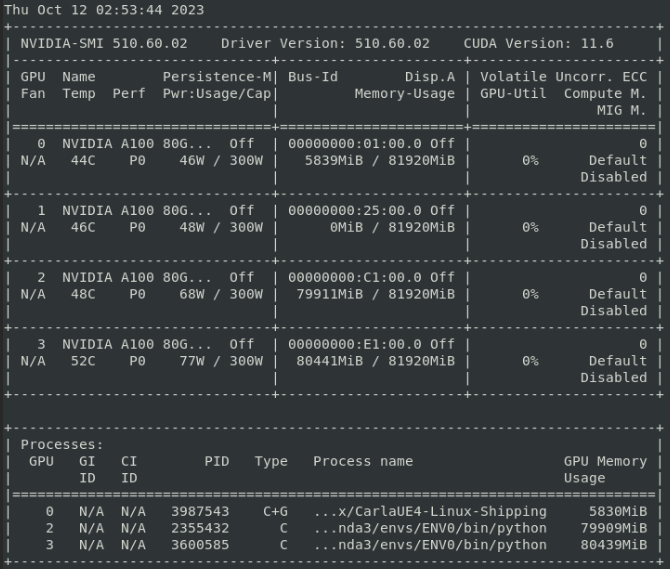
\includegraphics[height=9cm]{imagenes/cap3/graficas.png}
	\end{center}
	\caption[carla to ros bridge]{información de las GPU del servidor Landau}
	\label{fig:graficas servidor landau}
\end{figure}


\bigskip

De esta manera y después de que me fueran otorgados los permisos para acceder a este servidor, este se convirtió en un pilar casi imprescindible de este \ac{TFG} debido a que fue en esta plataforma donde se ejecutaron CARLA y todos los algoritmo y aplicaciones de conducción autónoma de una manera lo suficientemente fluida como para permitir un comportamiento reactivo.

\newpage
	











\chapter{Diseño}
\label{cap:capitulo4}

El \ac{TFG} que a continuación se describe tiene como objetivo realizar una investigación sobre la conducción autónoma mediante \ac{IA}, más concretamente mediante aprendizaje por refuerzo. Se tomará como entorno base el simulador foto-realista CARLA. Adicionalmente, se profundizará en la sinergia entre CARLA y ROS 2, evaluando en particular la eficacia y viabilidad del \textit{CARLA to ROS bridge}, herramienta que se encarga de actuar como 'puente' entre estos dos programas, permitiendo que puedan comunicarse de manera efectiva entre sí. Además, también se evaluará la fusión de ROS  2 y CARLA como herramienta esencial en el diseño de soluciones integradas y robustas para la conducción autónoma

\bigskip

Dentro del contexto de la conducción autónoma primero se exploran distintas soluciones para un sistema de seguimiento de carril con un enfoque tradicional. La detección de carril en este sistema se basará en métodos fundamentados en la visión artificial y el procesamiento de imágenes. A pesar de que estos algoritmos no son considerados de vanguardia en la actualidad, desempeñaron un papel fundamental en los primeros desarrollos de vehículos autónomos. Posteriormente estos métodos más tradicionales se compararán con otro sigue carril cuya percepción este basada en una red neuronal. En ambos casos el control del vehículo para el seguimiento del carril estará gobernado por un controlador \ac{PID}
\bigskip

Después de exponer estos dos enfoques para crear un sigue carril, con distintos métodos de percepción unos tradicionales y otro más moderno, en los cuales se utiliza el mismo tipo de controlador para gestionar los movimientos, se recopilarán datos con los cuales se generarán gráficos que nos permitirán hacer análisis que destacará las fortalezas y debilidades de cada técnica en diversas situaciones y contextos de conducción a la hora de filtrar y detectar de carriles. Este análisis arrojará luz sobre qué método es más efectivo y robusto para esta tarea, permitiendo así tomar una decisión fundamentada sobre cuál método elegir en las soluciones finales de conducción autónoma.

\bigskip

Finalmente, el \ac{TFG} concluirá con la creación de tres algoritmos avanzados de seguimiento de carril en los cuales la detección del carril y estará a cargo del método de percepción seleccionados después de los dos análisis anteriores y el control del vehículo estará a cargo de un algoritmos basado en aprendizaje por refuerzo.

\bigskip

El primer algoritmo estará especialmente diseñado para seguir carriles de manera efectiva para seguir carriles de manera fluida, segura y reactiva en carreteras despejadas. El segundo algoritmo estará especialmente diseñado para además de seguir carriles de manera efectiva evitar colisiones con otros vehículos u objetos en caso de encontrarlos en la vía frenando y deteniendo la marcha, garantizando así una conducción segura en entornos con posibles obstáculos. El tercer algoritmo será una versión mejorada del Segundo. Además de frenar para evitar colisiones con obstáculos, el vehículo se adaptará a la velocidad de los obstáculos en caso de que estos estén en movimiento, de modo que no se produzcan colisiones, pero sin llegar a detener el vehículo por completo. Esto creará un sistema capaz de adaptarse de manera efectiva a situaciones de tráfico dinámico.


\section{Arquitectura}

\begin{figure} [h]
	 \center
	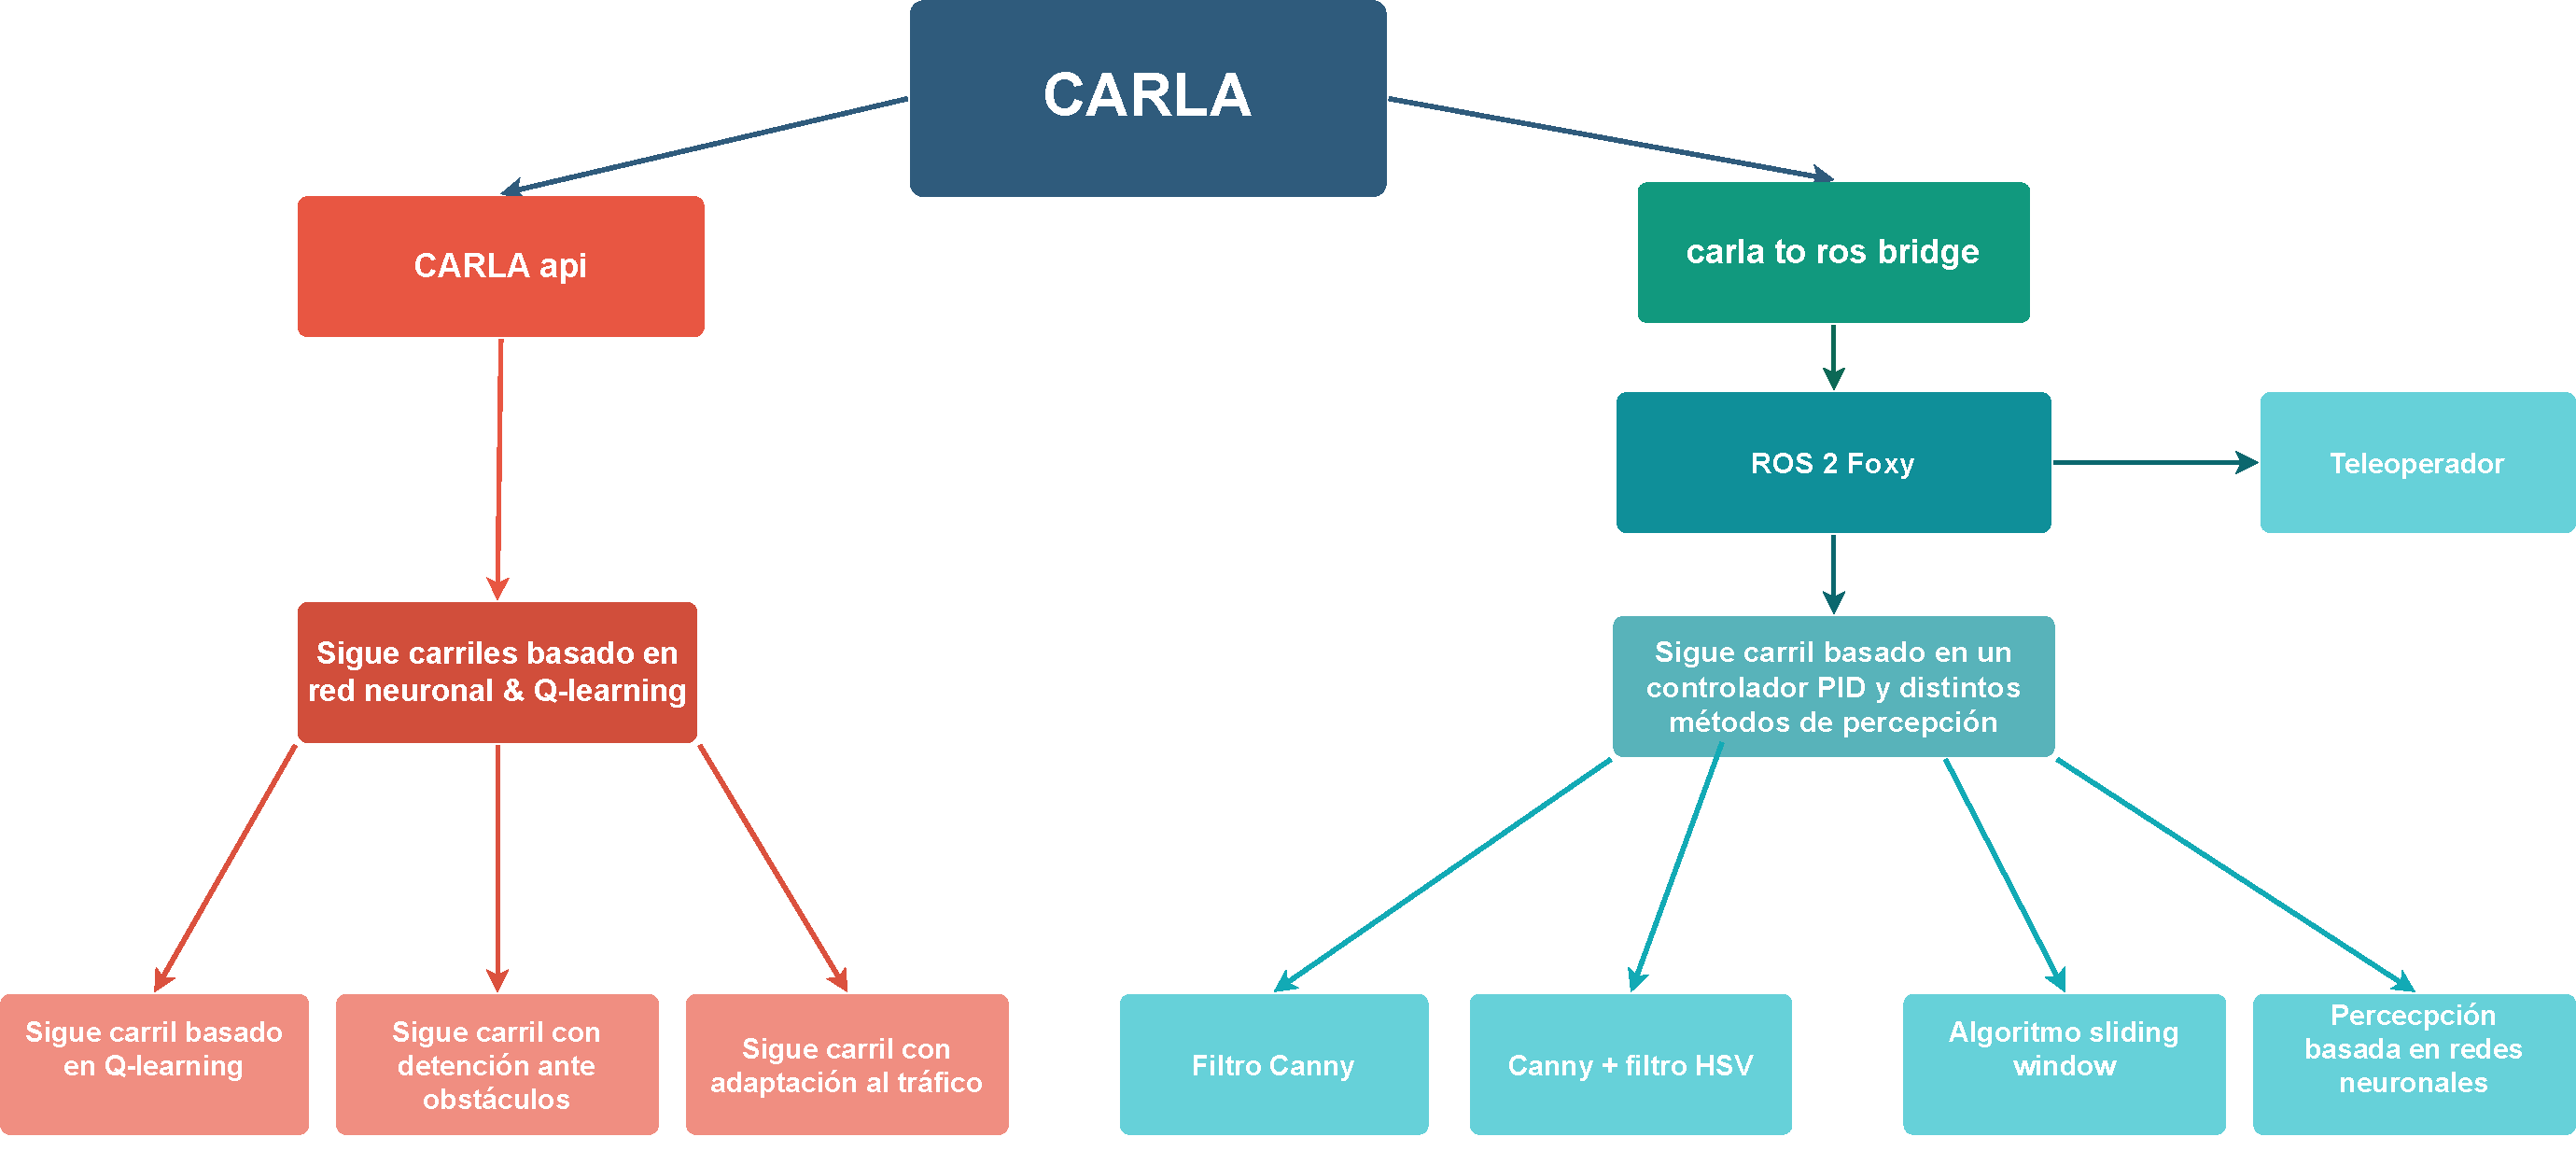
\includegraphics[height=7cm]{imagenes/cap4/Arquitectura.pdf}
	\caption[Arquitectura de los elementos que componen el TFG ]{Arquitectura de los elementos que componen el TFG}
	\label{fig:Arquitectura del TFG}
\end{figure}

La arquitectura de este \ac{TFG} se compone de varios elementos clave que se integran para llevar a cabo la investigación y el desarrollo de las soluciones de seguimiento de carril. En la figura \ref{fig:Arquitectura del TFG} se puede ver una descripción general de esta arquitectura.


\bigskip

Como se puede observar en la figura \ref{fig:Arquitectura del TFG} el entorno de simulación CARLA sirve como el denominador común y la plataforma central para la realización de pruebas y evaluación de algoritmos.

\bigskip

 Una gran cantidad de las implementaciones de sigue carril que se presentan en este \ac{TFG} se han desarrollado en el entorno de ROS 2 el cuál se comunica con CARLA a través del puente \textit{CARLA to ROS bridge} como ya se ha comentado en anteriores ocasiones. Estas implementaciones incluyen:

\bigskip

\begin{itemize}
  \item \textbf{Teleoperador}: Permite el control manual del vehículo en el entorno CARLA a través de topics de de ROS 2.

  \item \textbf{Algoritmo de Seguimiento de Carril basado en Canny + \ac{PID}}: Utiliza el algoritmo de detección de bordes Canny y un controlador \ac{PID} para el seguimiento de carriles.

  \item \textbf{Algoritmo de Seguimiento de Carril basado en Canny + Filtro de Color HSV + \ac{PID}}: Combina la detección de bordes Canny con un filtro de color basado en espacio de color HSV y un controlador \ac{PID} para el seguimiento de carriles.

  \item \textbf{Algoritmo de Seguimiento de Carril basado en Sliding Window + \ac{PID}}: Utiliza un pipeline de procesamiento de imagen con un algoritmo sliding window junto con un controlador \ac{PID} para el seguimiento de carriles.

  \item \textbf{Algoritmo de Seguimiento de Carril basado en Redes Neuronales + \ac{PID}}: Implementa un sistema de seguimiento de carriles basado en redes neuronales convolucionales y utiliza un controlador \ac{PID} para el control del vehículo.
\end{itemize}

\bigskip

Por otro lado Además de las implementaciones en ROS, se han desarrollado también diferentes programas en la \ac{API} del lenguaje Python de CARLA que se ejecutan directamente en el entorno de simulación CARLA, más adelante en la sección \ref{Sigue carriles basado en redes neuronales y Qlearnig} se explica porque se tomó esta decisión. Estas implementaciones incluyen:

\bigskip

\begin{itemize}
  \item \textbf{Seguimiento de Carril basado en Redes Neuronales y Q-learning}: Utiliza una red neuronal junto con el algoritmo de aprendizaje por refuerzo y Q-learning para el seguimiento de carriles.

  \item \textbf{Seguimiento de Carril basado en Redes Neuronales, Q-learning y Detección de Obstáculos}: Amplía la implementación anterior al detener el vehículo si se detecta un obstáculo en la vía.

  \item \textbf{Seguimiento de Carril Adaptativo al Tráfico}: Implementa un sistema de seguimiento de carriles que se adapta al tráfico.
\end{itemize}

\bigskip


\section{Instalación del entorno de trabajo}
\label{Instalación del entorno de trabajo}

Este \ac{TFG} comenzó con la búsqueda y lectura de documentación e información relevante sobre todos los componentes del entorno de trabajo en el cual se iba a desarrollar el \ac{TFG}. Posteriormente, se procedió con la instalación de todos los programas necesarios para crear dicho entorno: el simulador foto-realista de conducción autónoma CARLA, el sistema operativo robótico ROS 2 y el `puente' para comunicar ambos, el \textit{CARLA to ROS bridge.}

\subsection{Instalación de CARLA}
\label{Instalación de CARLA}

Para la instalación de CARLA, el procedimiento consiste en seguir las directrices de instalación detalladas en la página oficial del simulador\footnote{\url{https://carla.org/}}.

\bigskip

En primer lugar, se añadió el repositorio Debian de CARLA al sistema utilizado para trabajar.
 
   \begin{code}[H]
	\begin{lstlisting}[language=sh]
    sudo apt-key adv --keyserver keyserver.ubuntu.com --recv-keys 1AF1527DE64CB8D9
    sudo add-apt-repository "deb [arch=amd64] http://dist.carla.org/carla $(lsb_release -sc) main"
	\end{lstlisting}
\caption[Añadir repositorio de CARLA al sistema]{Añadir repositorio de CARLA al sistema}
\label{cod:Añadir repositorio de CARLA al sistema}
\end{code}

A continuación, se procedió a la instalación de la última versión de CARLA disponible utilizando el siguiente comando:


   \begin{code}[H]
	\begin{lstlisting}[language=sh]
    sudo apt-get update
    sudo apt-get install carla-simulator
	\end{lstlisting}
\caption[Comandos para instalar la versión más reciente de CARLA]{Comandos para instalar la versión más reciente de CARLA}
\label{cod:Comandos para instalar CARLA}
\end{code}


Después de completar la instalación del simulador, el siguiente paso, como era de esperar, fue ejecutarlo y verificar su correcto funcionamiento. Fue en este punto donde surgió el primer problema en este \ac{TFG}. A pesar de estar ejecutándolo en una máquina con una potente tarjeta gráfica dedicada, específicamente una NVIDIA RTX 3060 para portátiles, el simulador utilizaba automáticamente la tarjeta gráfica integrada del ordenador. Esto resultó en una simulación extremadamente lenta, con poca fluidez y una tasa de fotogramas muy baja de alrededor de 3 \ac{FPS}.

\bigskip

La solución para este problema se encontró en una respuesta a una entrada en un \textit{issue} en el GitHub oficial de CARLA\footnote{\url{https://github.com/carla-simulator/carla/issues/4716}} que hacía referencia a un problema similar. Se descubrió que al ejecutar CARLA con la flag -prefernvidia, el simulador podía ser forzado a utilizar la tarjeta gráfica NVIDIA en caso de que estuviera disponible en el equipo. A partir de este punto, el comando utilizado para ejecutar CARLA durante toda la fase de este \ac{TFG} que se llevo a cabo en la maquina mencionada fue el siguiente:

   \begin{code}[H]
	\begin{lstlisting}[language=sh]
		/opt/carla-simulator/CarlaUE4.sh -prefernvidia
	\end{lstlisting}
\caption[Comando para lanzar el simulador CARLA]{Comando para lanzar el simulador CARLA}
\label{cod:Comando para lanzar el simulador CARLA}
\end{code}
 

\subsection{Instalación de ROS 2}
\label{Instalación de ROS 2}

Una vez instalado el simulador CARLA, el siguiente elemento necesario en el entorno de trabajo era ROS 2. Como se explica en su documentación oficial \cite{distribuciones_ros}, ROS 2 se divide en una serie de versiones específicas de paquetes ROS 2 que se publican en momentos concretos llamadas distribuciones. Por lo tanto, una tarea importante antes de instalar ROS 2 era elegir qué distribución se iba a utilizar. Debido a que ya se había trabajado con ella anteriormente en otros proyectos y que es una versión estable y probada, se eligió ROS 2 Foxy \footnote{\url{https://docs.ros.org/en/foxy/index.html}} como la distribución para desarrollar el \ac{TFG}.

\bigskip

Una vez que se tuvo claro qué versión de ROS 2 se utilizaría, se navegó hasta la página oficial de ROS 2 Foxy para seguir los pasos de instalación\footnote{\url{https://docs.ros.org/en/foxy/Installation.html}}. De los dos métodos que se presentan en la página web, se eligió el método de instalación mediante paquetes DEB\footnote{\url{https://wiki.debian.org/deb}}.

\begin{figure} [H]
	\begin{center}
	
\includegraphics[height=8cm]{imagenes/cap4/ros_2_foxy.png}
	\end{center}
	\caption[Logotipoo de ROS 2 foxy]{Logotipo de ROS 2 foxy}
	\label{fig:logotipo_ros_2_foxy}
\end{figure}


\subsection{Instalación de CARLA to ROS Bridge}
\label{carla-to-ros-bridge}

Como se ha mencionado previamente en este documento, CARLA y ROS 2 no están diseñados para funcionar conjuntamente de forma nativa. Para que estos dos programas puedan trabajar juntos, es necesario que puedan comunicarse de alguna manera. Para lograr esto, los desarrolladores de CARLA ofrecen una herramienta muy interesante: \textit{CARLA to ROS bridge}. Este programa se encarga, tal como se menciona en su repositorio oficial en GitHub\cite{carla_to_ros_bridge}, de crear un método de comunicación bidireccional entre ROS 2 y CARLA, permitiendo una simbiosis entre ambos.

\bigskip

Las instrucciones de instalación de CARLA to ROS bridge se encuentran en una sección de la documentación oficial del simulador CARLA\footnote{\url{https://carla.readthedocs.io/projects/ros-bridge/en/latest/}}. No obstante, la instalación y el método de uso son bastante sencillos. Primero se debe clonar el repositorio de GitHub de CARLA to ROS bridge en el proyecto ROS en el que deseamos utilizarlo. Esto se puede realizar con el siguiente comando:

  \begin{code}[H]
	\begin{lstlisting}[language=sh]
	git clone https://github.com/carla-simulator/ros-bridge.git 
 
	\end{lstlisting}
\caption[git clone de CARLA to ROS bridgel ]{git clone de CARLA to ROS bridge}
\label{cod:git clone de carla to ros bridge}
\end{code}

 Una vez clonado el repositorio para poder utilizarlo en un proyecto, es necesaria su inclusión en el archivo CMakeList.txt como se enseña en el código \ref{cod:Como incluir CARLA to ros bridge en un CMakeList.txt}

 
 \begin{code}[H]
	\begin{lstlisting}[language=Python]
	
 find_package(catkin REQUIRED ...
  carla_ros_bridge  
  ...
)
 
 catkin_package(
  ...
  CATKIN_DEPENDS
    ...
    carla_ros_bridge
    ...
)
	\end{lstlisting}
\caption[Como incluir CARLA to ros bridge en un CMakeList.txt ]{Como incluir CARLA to ros bridge en un CMakeList.txt}
\label{cod:Como incluir CARLA to ros bridge en un CMakeList.txt}
\end{code}
 
Después de configurar el  CMakeList.txt, solo se tendrá que incluir en el nodo ROS 2 que necesite comunicarse con CARLA las funciones, tipos de mensajes, etc. que vayamos a requerir del ROS bridge, y luego compilar el paquete de manera habitual.

\bigskip

En el código \ref{cod:Ejemplo de uso del carla to ros bridge}, se presenta un código de ejemplo escrito en Python para la plataforma ROS 2 Foxy que realiza la acción de comandar a un vehículo de CARLA mediante un publicador de ROS, utilizando el valor máximo posible de aceleración del vehículo.

  \begin{code}[H]
	\begin{lstlisting}[language=Python]
	
import rclpy
from carla_msgs.msg import CarlaEgoVehicleControl

self.vehicle_control_publisher = self.create_publisher( CarlaEgoVehicleControl, "/carla/ego_vehicle/vehicle_control_cmd", 10)       
       
self.control_msg = CarlaEgoVehicleControl()

self.control_msg.throttle = 1.0
self.control_msg.steer = 0.0 
self.control_msg.brake = 0.0
self.control_msg.hand_brake = False
self.control_msg.reverse = False
self.control_msg.gear = 0

 self.vehicle_control_publisher.publish(self.control_msg)
 
	\end{lstlisting}
\caption[Ejemplo de uso del CARLA to ROS bridge ]{Ejemplo de uso del CARLA to ROS bridge}
\label{cod:Ejemplo de uso del carla to ros bridge}
\end{code}

\section{Creación de un teleoperador}

Tras la puesta a punto del entorno de trabajo, ya era posible comenzar a desarrollar el cuerpo del \ac{TFG}. No obstante, la conducción autónoma es una tarea muy compleja en la que intervienen numerosos factores y variables. Aventurarse en ella sin un conocimiento previo podría dejarte enfrentando un mundo inhóspito y desconocido en el cuál muy probablemente podrías acabar perdido. Además de esto, se añade la complicación de trabajar en un entorno que integra dos programas que no están explícitamente diseñados para trabajar juntos, como son ROS 2 y CARLA. Este hecho agrega un nivel adicional de dificultad a una tarea muy compleja de por sí.

\bigskip

Debido a esto, el desarrollo de este \ac{TFG} comienza con una pequeña tarea de iniciación que proporciona una primera toma de contacto con el entorno de trabajo y que nos dota de los conocimientos, las herramientas y la soltura necesarios para, posteriormente, afrontar las tareas principales de este \ac{TFG} de manera fluida y precisa. Esta tarea inicial debe ser algo que permitiera practicar con el control de vehículos de CARLA y su entorno, con la comunicación de CARLA con el ROS bridge y con los métodos para enviar comandos de control a CARLA desde ROS 2. Teniendo todo esto en cuenta, la tarea que resultó más adecuada para satisfacer todos estos requisitos fue la creación de un teleoperador para un vehículo de CARLA en ROS 2.

\subsection{Teleoperador en CARLA basado en ROS 2}
\label{Teleoperador en CARLA basado en ROS2}

El primer paso del desarrollo del teleoperador fue lanzar un mundo de CARLA generando en él, además, un vehículo que controlar. Para esto, nos ayudamos de un launcher ya presente en el repositorio de \textit{CARLA to ROS bridge}, más concretamente del launcher \textbf{carla\_generate\_vehicle.launch.py}. Este launcher se encarga de lanzar tanto el mundo de CARLA en una ciudad definida, como un vehículo de la librería de vehículos disponibles en CARLA, en este caso, un vehículo Tesla, como también el \textit{CARLA to ROS bridge} que a su vez se encarga de publicar todos los topics asociados al vehículo lanzado para poder interactuar con él desde ROS 2.

\bigskip

El control de un vehículo en CARLA se asemeja en gran medida a la operación de un vehículo real. En lugar de simplemente enviar comandos de velocidad lineal, se controla la cantidad de empuje que se comanda al vehículo o la cantidad de fuerza de freno que se aplica, esto equivale a la cantidad de presión que se le aplica al acelerador o al freno en un automóvil real. Además, la dirección del vehículo se controla indicando la cantidad de giro que se debe aplicar al volante del vehículo, estas características de control, sin duda añaden un nivel adicional de complejidad en comparación a otro tipo de simuladores.

\bigskip
Es importante destacar que, en CARLA, también se tiene la capacidad de controlar las marchas del vehículo. Sin embargo, para simplificar nuestras pruebas y evitar complicaciones innecesarias, se ha optado por utilizar un vehículo automático en lugar de uno con transmisión manual para esta y para todas las aplicaciones que de desaroolan en este \ac{TFG}.
\bigskip

El siguiente paso fue crear una interfaz gráfica para visualizar y controlar el vehículo de CARLA. En este caso, se utilizó la librería de Python pygame \footnote{\url{https://www.pygame.org/wiki/GettingStarted}} ya mencionada en la sección \ref{subsec:Pygame}. Pygame resultaba resultaba una opción perfecta para crear una interfaz gráfica en la que se visualizarían imágenes del vehículo y que además nos permitiera controlar sus movimientos al presionar el teclado, ya que en cierta medida esto es algo bastante parecido a lo que podría ser un videojuego.

\bigskip

Para implementar  la \ac{GUI} se creó una ventana en Pygame, la cual se dividió en dos partes por la mitad. En la mitad izquierda se visualizaría el vehículo visto desde una perspectiva de tercera persona, mientras que en la mitad derecha se mostraron las imágenes de la cámara frontal con la que iba equipado el vehículo. Esta cámara se encontraba ubicada en el capó del vehículo, justo en la parte media de este.. Adicionalmente, en la parte superior izquierda de la mitad derecha, también se añadió un pequeño indicador que mostraba la tasa de refresco de \ac{FPS} de la imagen. El resultado final de la interfaz se puede ver en la figura \ref{fig: GUI de un teleoperador para un vehículo de CARLA}.

\begin{figure}[h]
    \centering
    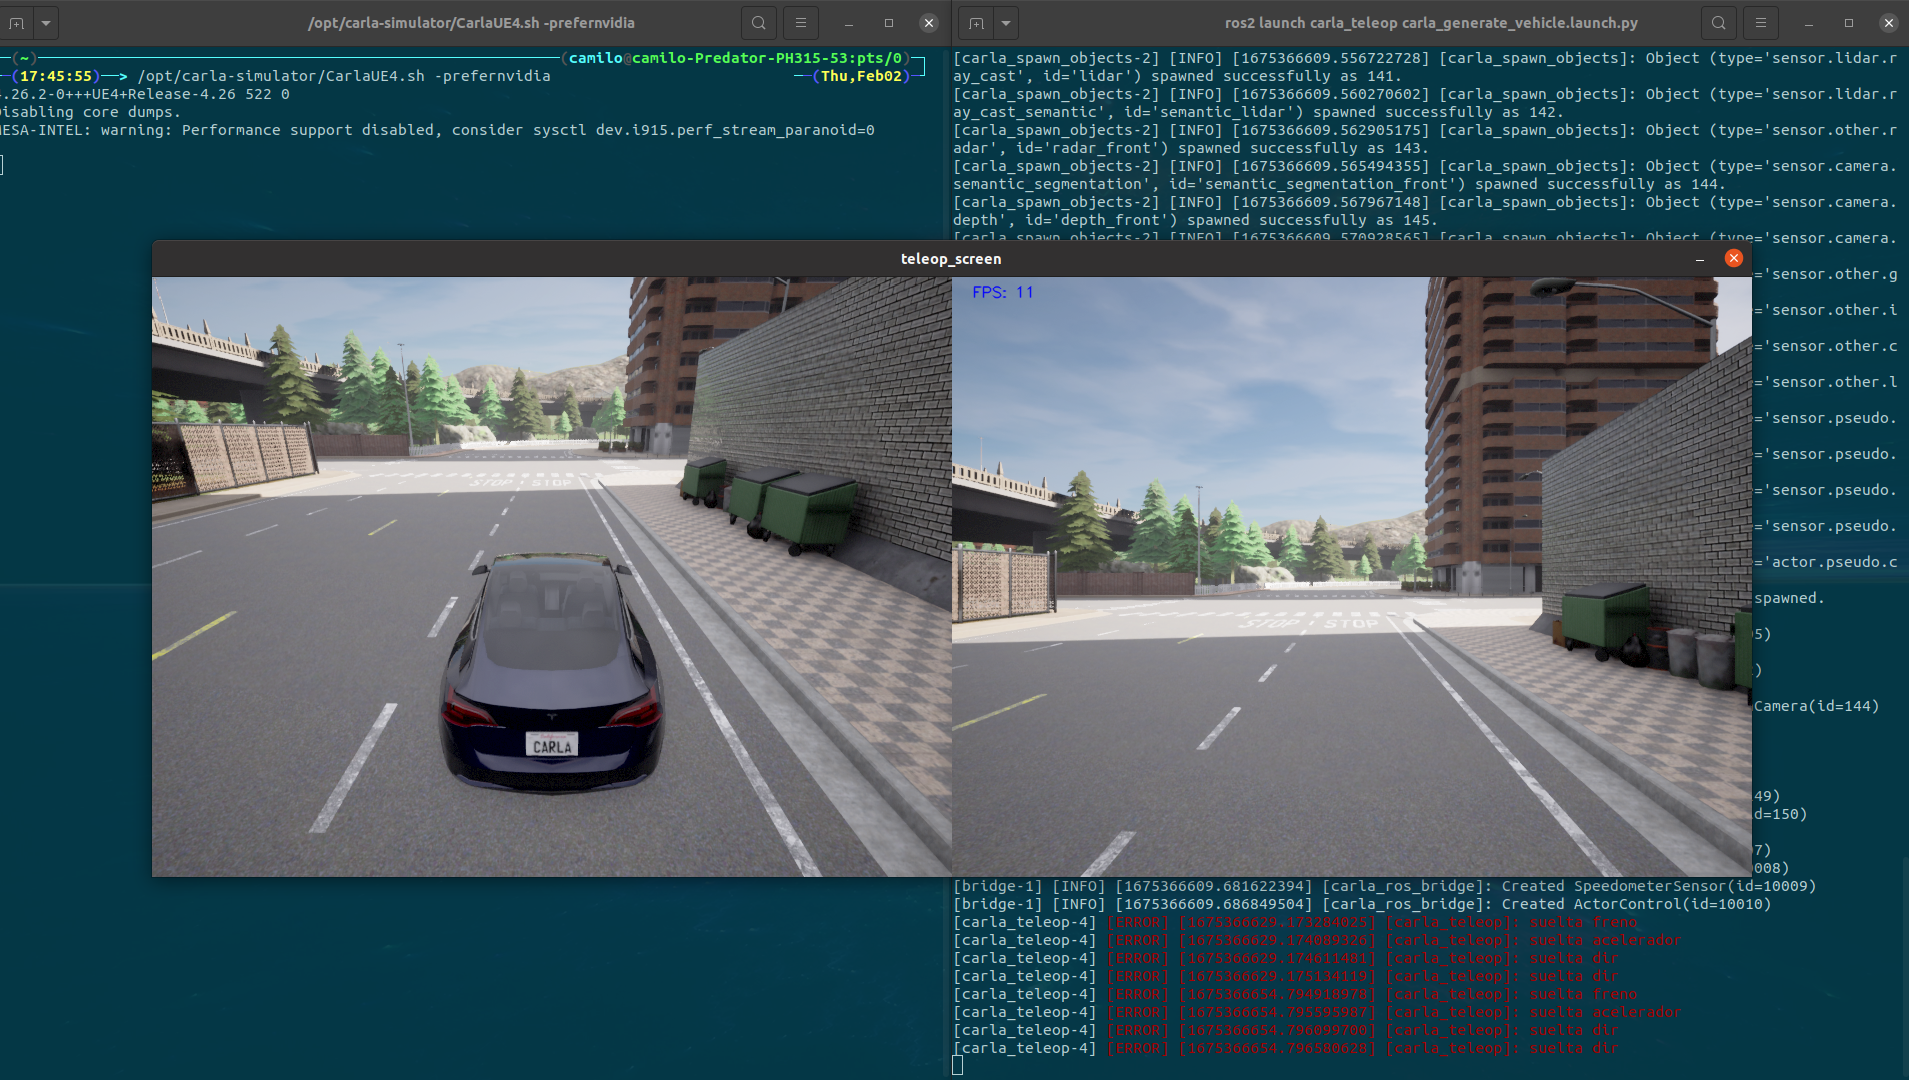
\includegraphics[height=8cm]{imagenes/cap4/vehicle_teleop_hmi.png}
    \caption{GUI de un teleoperador para un vehículo de CARLA}
    \label{fig: GUI de un teleoperador para un vehículo de CARLA}
\end{figure}

\bigskip

Una vez finalizado la \ac{GUI} de esta aplicación nos encontramos con la primera limitación del \textit{CARLA to ROS bridge}. Y es que a pesar de que el simulador CARLA por si solo funciona a unos 60 \ac{FPS} en la máquina que se estaba desarrollando la aplicación, las imágenes recibidas por la \ac{GUI} luego de que estas fueran traducidas de CARLA a ROS 2 a través del ROS bridge no superaban los 15 \ac{FPS}. Tras investigar se descubrió qué esto se debe a un cuello de botella que genera el \textit{CARLA to ROS bridge}, en las imágenes que traduce de CARLA. Todas las imágenes que \textit{CARLA to ROS bridge} traduzca a ROS 2 mediante topics tienen un límite máximo de tasa de refresco de alrededor de 15 \ac{FPS}. Este problema significa que ninguna de las aplicaciones que se hagan utilizando CARLA y ROS 2 con el ROS bridge como método de comunicación podrán superar este frame rate máximo, un problema sin duda muy grave cuando hablamos de conducción autónoma ya que a altas velocidades necesitamos buenas tasas de refresco de \ac{FPS} para poder ser reactivos y adaptarnos a cambios repentinos. A pesar de esto a velocidades no muy altas 15 \ac{FPS} resultan suficientes para tener un comportamiento fluido

\bigskip

Terminada la \ac{GUI} del teleoperador, se prosiguió implementando el control del vehículo para poder manejarlo utilizando el teclado del computador. Para realizar esta tarea, se utilizaron los eventos de pygame \footnote{\url{https://www.pygame.org/docs/ref/event.html}}. Mediante estos eventos es posible capturar qué teclas del teclado se están presionando en cada momento. Posteriormente, se asoció una serie determinada de teclas al control del vehículo. Esta implementación puede verse con más claridad en el código \ref{cod:Eventos de pygame para controlar el teleoperador} De esta manera, cada vez que se apretaba una de estas teclas, se publicaba en los topics del vehículo la acción asociada a esa tecla. Luego, era trabajo del \textit{CARLA to ROS bridge} traducir los mensajes de estos topics a comandos de CARLA.


  \begin{code}[H]
	\begin{lstlisting}[language=Python]
    def control_vehicle(self):        
    
        self.set_autopilot()
        self.set_vehicle_control_manual_override()

        while True:
            for event in pygame.event.get():

                if event.type == KEYDOWN:
                    keys = pygame.key.get_pressed()

                    if (keys[K_DOWN]):
                        self.control_msg.brake = 1.0
		
                    if (keys[K_UP]):
                        self.control_msg.throttle = 1.0          

                    if (keys[K_LEFT]):
                        self.control_msg.steer = -1.0            

                    if (keys[K_RIGHT]):
                        self.control_msg.steer = 1.0
                        
            self.vehicle_control_publisher.publish(self.control_msg)

	\end{lstlisting}
\caption[Eventos de pygame para controlar el teleoperado]{Eventos de pygame para controlar el teleoperador}
\label{cod:Eventos de pygame para controlar el teleoperador}
\end{code}


\bigskip

Finalmente, para que el procesamiento de los eventos de Pygame no interfiriera con el procesamiento de las imágenes del vehículo, cada una de estas funcionalidades fue implementada en un hilo distinto. De esta manera, un hilo del programa controla la \ac{GUI} y la visualización de imágenes, mientras que el otro controla el manejo del vehículo mediante el teclado.

\bigskip

En este \href{https://roboticslaburjc.github.io/2022-tfg-juancamilo-carmona/DEMOS/}{\textbf{post}} del blog creado para el seguimiento de este \ac{TFG} se puede encontrar un video demostración del funcionamiento del teleoperador.

\bigskip


\section{ Sigue carril basado en un controlador PID y distintos métodos de percepción}
\label{ Sigue carriles basado en visión artificial y un controlador PID }

Tras finalizar esta tarea inicial, como era lógico y esperado, observamos un aumento significativo en nuestra familiaridad con el entorno. La interacción entre ROS 2 y CARLA se tornó  más intuitiva, resaltando así que se habían adquirido las competencias fundamentales necesarias para trabajar de manera cómoda y fluida con estos dos programas. Con esta base establecida, nos encontrábamos en una posición óptima para empezar con el desarrollo de las tareas principales del \ac{TFG}.

\bigskip

Como nuestra misión es determinar que algoritmo nos proporciona una mejor detección de carril, en todos lo métodos se utilizará el mismo controlador para manejar la dirección y velocidad lineal del vehículo para lograr el comportamiento de seguimiento de carril. Este controlador consistirá en una implementación de un controlador \ac{PID}. Un controlador \ac{PID} es un controlador que ajusta un sistema para minimizar el error entre una variable medida y su valor deseado, utilizando tres componentes: proporcional (P), integral (I) y derivativo (D). Es ampliamente usado en sistemas de control industrial y robótica.

\bigskip

 En todos los métodos se seguirá la siguiente dinámica: Primero se filtrarán las dos líneas que delimitan el carril utilizando un método de filtrado de cada implementación, a continuación se calculará el centro del carril filtrado en la carretera, posteriormente este centro se comparará con el centro de la imagen, calculando el error que hay entre ambos. Este error será el error del controlador \ac{PID}, de esta manera se consigue que el controlador \ac{PID} siempre procure mantener el centro del carril alineado con el centro de la imagen ya que en este caso el error sería igual a 0 y como en nuestro vehículo la cámara se localiza en el centro del capó, mantener el centro del carril y el centro de la imagen alineados genera que el centro del vehículo se mantenga en el centro del carril evitando así que el vehículo se salga del carril. Para obtener una mayor adaptabilidad el controlador \ac{PID} utilizará constantes ki, Kp y Kd distintas para situaciones con carriles rectos o con curvas muy suaves y para situaciones con curvas más pronunciadas. Los valores específicos utilizados se pueden ver en el código \ref{cod:controlador_PID_visión_artificial}

\begin{code}[H]
	\begin{lstlisting}[language=Python]
        self.kp_straight = 0.07
        self.kd_straight  = 0.09
        self.ki_straight = 0.000003
        
        self.kp_turn = 0.1
        self.kd_turn= 0.15
        self.ki_turn = 0.000004
	\end{lstlisting}
\caption[Constantes del controlador PID]{Constantes del controlador PID}
\label{cod:controlador_PID_visión_artificial}
\end{code}

\bigskip

Además del controlador que mantendrá al vehículo dentro del carril, para que el vehículo avance por este se le otorgará una velocidad lineal fija, que se mantendrá durante todo el recorrido y que no variará manteniéndose lo más estable posible. Esta velocidad será de 20 km/h. Como ya se explicó antes en CARLA el movimiento del vehículo se controla mediante el empuje y no comandando una velocidad lineal, por lo que para mantener una velocidad fija se ha diseñado un pequeño controlador para aplicar empuje cuando la velocidad baje de la deseada y dejar de aplicarlo cuando supere la misma. Su implementación se puede ver en el código \ref{cod:Controlador de velocidad fija del vehículo}

\begin{code}[H]
	\begin{lstlisting}[language=Python]
	
	if self.speed >= 20:
		self.control_msg.throttle = 0.0            
	else:
		self.control_msg.throttle = 1.0    
	\end{lstlisting}
\caption[Controlador de velocidad fija del vehículo]{Controlador de velocidad fija del vehículo}
\label{cod:Controlador de velocidad fija del vehículo}
\end{code}


\subsection{Método de percepción 1: Filtro Canny}
\label{Método 1: Filtro Canny}

El primer método utilizado para detectar el carril se basa en un enfoque muy básico. En este método, se utilizará un filtro Canny. Canny es un algoritmo que, mediante la detección de cambios abruptos de intensidad utilizando cálculos de gradientes y umbralización, es capaz de detectar bordes en una imagen. Este filtro resulta especialmente útil en nuestro caso, ya que nos ofrece la posibilidad de detectar los bordes que delimitan las líneas del carril en nuestra carretera.

\bigskip

Después de filtrar las líneas del carril con Canny, se delimita un área de interés en la que el carril debería localizarse para, de esta manera, eliminar el ruido de posibles interferencias generadas por el propio entorno fuera de nuestra zona de interés, edificios, arboles, carteles etc. y finalmente se utilizará la función de OpenCV HoughLinesP\footnote{\url{https://docs.opencv.org/3.4/d3/de6/tutorial_js_houghlines.html}} para detectar estas líneas ya filtradas y guardar los píxeles que las componen. Esto nos permitirá posteriormente analizarlos con la finalidad de encontrar el centro del carril y controlar nuestro vehículo. La  implementación de este método de filtrado de carril se puede observar en el código \ref{cod: filtro canny}

  
\begin{code}[H]
	\begin{lstlisting}[language=Python]
	
    def line_filter(self, img):
        gray_image = cv2.cvtColor(img, cv2.COLOR_RGB2GRAY)
        
        #apply canny filter
        cannyed_image = cv2.Canny(gray_image, 100, 150)
       
       #crop interest region
        h, w = cannyed_image.shape[:2]
        region_of_interest_vertices = [ (0, h*0.7),(w/2 , h/2) ,(w, h*0.7), ]
        cropped_image = self.region_of_interest(cannyed_image, numpy.array([region_of_interest_vertices], numpy.int32))
        
       #detect lines with Houghlines
        lines = cv2.HoughLinesP(cropped_image,rho=9,theta=numpy.pi / 60, threshold=50,lines=numpy.array([]),minLineLength=20,maxLineGap=25)
	\end{lstlisting}
\caption[Implementación de filtro canny ]{Filtro canny}
\label{cod: filtro canny}
\end{code}
  
Como se puede observar en el código \ref{cod: filtro canny} primero aplicamos el filtro Canny a las imágenes obtenidas de la cámara, luego recortamos la zona de interés anteriormente mencionada y finalmente aplicamos Houghlines para detectar y guardar las coordenadas de las lineas. Este método tiene la ventaja de que al ser muy sencillo resulta computacionalmente muy ligero, ya que el único procesamiento de imagen que se realiza es un simple Canny y posteriormente la detección de líneas mediante Houghlines.

\bigskip

Pero por otro lado nuevamente al ser un método tan sencillo el filtro de carril no es muy robusto y presenta numerosas limitaciones un ejemplo del filtrado de un carril con este método puede verse en la figure \ref{fig:Carril filtrado con método canny}. En muchas ocasiones carril de la vía no se llega a filtrar adecuadamente, además de la aparición de fallos y errores de detección en muchos momentos sobretodo al intentar filtrar líneas discontinua. A pesar de esto, con este método se puede conseguir un comportamiento de sigue carril relativamente fluido en un entorno controlado. En esta entrada \href{https://roboticslaburjc.github.io/2022-tfg-juancamilo-carmona/DEMOS/}{\textbf{entrada}} del blog del \ac{TFG} se puede encontrar un video donde se observa el funcionamiento de este método.

\begin{figure} [t]
	\begin{center}
	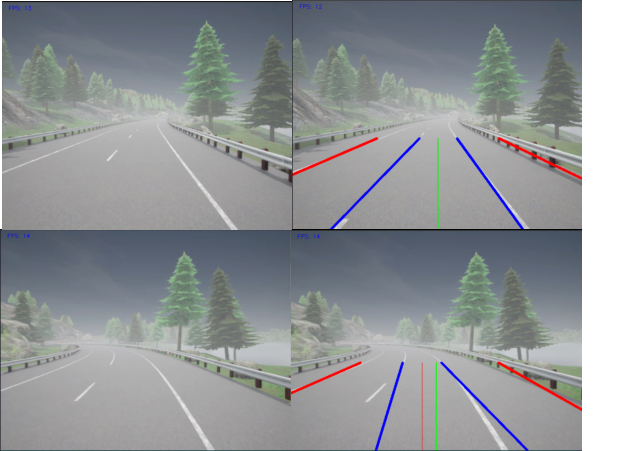
\includegraphics[height=8cm]{imagenes/cap4/graphichs_canny/filtro_carril.pdf}
	\end{center}
	\caption[Carril filtrado con método canny]{Carril filtrado con método de percepción basado en canny}
	\label{fig:Carril filtrado con método canny}
\end{figure}

\newpage

\subsection{Método de percepción 2: Filtro de color HSV + filtro Canny}
\label{Método 2: Filtro de color HSV + filtro Canny}

El segundo método utilizado para detectar el carril de la vía es una extensión del primero. En este método, nuevamente se utilizará la función de detección de líneas HoughLines y un filtro Canny, pero con el añadido de que ahora, además del filtro Canny, se añadirá una segunda función de filtrado de carril: un filtro de color. Las líneas que delimitan los carriles generalmente son de color blanco mientras que la carretera, por el contrario, es de color negro o gris. Esta clara diferencia de color entre ambos elementos permite detectar las líneas de la carretera filtrando los colores blancos de los negros y grises presentes en la imagen de la cámara.

\bigskip

Primero, antes de pasar a implementar este método, debemos determinar el rango de color que vamos a filtrar y en qué formato. En visión artificial, es común utilizar el formato HSV para filtros de color debido al control que ofrece sobre el contraste y la iluminación. Estas características se adaptan bien a nuestro caso, en el que no buscábamos separar diferentes colores, sino distinguir el negro del blanco. Para definir el espectro de color que deseábamos filtrar, posicionamos el vehículo de CARLA en diferentes ubicaciones del mapa y capturamos imágenes que la cámara recogía del carril. Una vez que teníamos estas imágenes, diseñamos una sencilla herramienta que mostrara la imagen en pantalla y nos permitiera ajustar los valores de HSV que se aplicaban a la imagen mediante controles deslizantes. Con esta herramienta, buscábamos encontrar un rango de valores HSV común a todas las imágenes que filtrara las líneas blancas del carril de la mejor manera posible.

\bigskip

Sin embargo, al realizar el filtrado de las líneas mediante HSV, nos encontramos con la primera limitación de este método. Debido al foto-realismo de las imágenes del simulador CARLA, los cambios de luz, sombras y reflejos eran comunes, y dependiendo de estos factores, el rango de color blanco de las líneas del carril variaba significativamente. Esto era especialmente evidente cuando el carril estaba expuesto a luz directa o cuando estaba bajo una sombra. En estos casos, era imposible filtrar las líneas del carril utilizando el mismo rango HSV.

\bigskip

Finalmente, concluimos que es imposible encontrar un rango de color blanco que fuera válido para todas las situaciones. Por lo tanto, intentamos encontrar un rango que abarcara el mayor número posible de situaciones. Luego de explorar muchos valores diferentes, elegimos el rango que se puede ver en el código \ref{cod: Filtro de color HSV}


\begin{code}[H]
	\begin{lstlisting}[language=Python]
        #HSV color filter range
        lower_white = numpy.array([0, 0, 200])
        upper_white = numpy.array([255, 255, 255])
	\end{lstlisting}
\caption[Rangos de detección del filtro de color HSV ]{ Rangos de detección del filtro de color HSV}
\label{cod: Rangos HSV}
\end{code}


 La implementación final del método de filtrado es la que se ve en el código \ref{cod: Filtro de color HSV}:

\begin{code}[H]
	\begin{lstlisting}[language=Python]
	
    def line_filter(self, img):

        hsv_image = cv2.cvtColor(img, cv2.COLOR_RGB2HSV)
        lower_white = numpy.array([0, 0, 200])
        upper_white = numpy.array([255, 255, 255])
	
        #apply HSV color filter
        color_mask = cv2.inRange(hsv_image, lower_white, upper_white)
        filtered_image = cv2.bitwise_and(img, img, mask=color_mask)
        
	\end{lstlisting}
\caption[Filtro de color HSVl ]{Filtro de color HSV}
\label{cod: Filtro de color HSV}
\end{code}

\bigskip


Con este método, nuevamente nos encontramos con la ventaja de que resulta ser computacionalmente muy ligero, ya que el único procesamiento añadido a la imagen es un simple filtro de color HSV. Esto se refleja en la tasa de \ac{FPS} de la imagen, ya que sigue sin variar mucho de los \ac{FPS} que obtenemos al mostrar una imagen sin procesamiento ni los que obtenemos en el método anterior. No obstante, debido al cuello de botella ya mencionado anteriormente, seguimos limitados a una tasa de refresco de 15 \ac{FPS}. Más tarde en la sección \ref{Comparación de los métodos de detección} se realizará un análisis más detallado de los \ac{FPS} y consumo de \ac{CPU} que realiza cada método

\bigskip

Se presenta nuevamente un enlace a una \href{https://roboticslaburjc.github.io/2022-tfg-juancamilo-carmona/DEMOS/}{\textbf{entrada}} del blog del \ac{TFG} en el que se puede encontrar un video donde se observa el funcionamiento de este método. Como vemos, el filtrado de las líneas del carril mejora ligeramente con respecto al método anterior; sin embargo, sigue siendo bastante defectuoso también podemos observar un ejemplo de filtrado de carril con este método en la imagen de la figura \ref{fig:Carril filtrado con método Canny + HSV}.

\begin{figure} [H]
	\begin{center}
	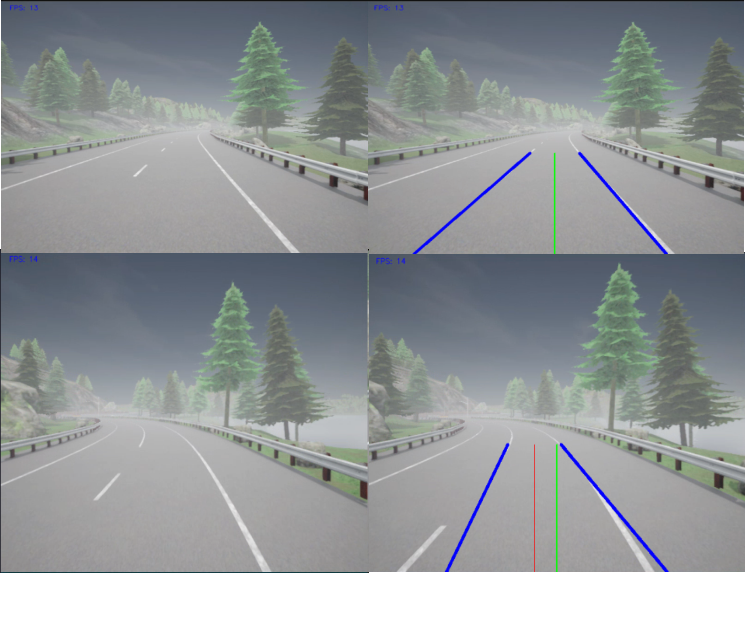
\includegraphics[height=8cm]{imagenes/cap4/graphics_hsv/carril_filtrado.pdf}
	\end{center}
	\caption[Carril filtrado con método Canny + HSV]{Carril filtrado con método de percepción canny + HSV}
	\label{fig:Carril filtrado con método Canny + HSV}
\end{figure}

\subsection{Método de percepción 3: Pipeline de procesamiento de imágenes con algoritmo Sliding window}
\label{Método 3: Pipeline de procesamiento de imágenes con algoritmo Sliding window}

Los dos primeros métodos que se han expuesto son métodos muy sencillos que no se suelen utilizar por si solos en soluciones del mundo real, ya que no aportan la robustez suficiente para funcionar en varios ambientes. El tercer método que vamos a utilizar para filtrar el carril es un método bastante más sofisticado y complejo con que los dos anteriores, a cambio este método promete entregarnos resultados más robustos y eficaces.

\bigskip

Este método consiste en un pipeline de varias transformaciones, filtros y procesamientos de imágenes que se le aplican a la imagen obtenida de la cámara, para filtrar el carril y guardar los píxeles en los que este se localiza. El pipeline utilizado es el siguiente:
\begin{enumerate}
    \item \textbf{Umbralización de color y gradiente:} Esta etapa consiste en una combinación de umbrales de color y gradiente para generar una imagen binaria de los carriles de la carretera.
    
    \item \textbf{Transformación de perspectiva:} La imagen es modificada para obtener una vista desde arriba o vista de pájaro de la imagen binaria de los carriles. Esto facilita la identificación y seguimiento de las líneas del carril al eliminar la perspectiva que podría distorsionar la percepción.
	
    \item \textbf{Algoritmo sliding window:} Al buscar las líneas del carril por primera vez o cuando el algoritmo tiene incertidumbre sobre las ubicaciones de las líneas, se realiza una búsqueda de ventanas mediante un algoritmo sliding window \footnote{\url{https://www.geeksforgeeks.org/window-sliding-technique/}}. Esta búsqueda toma un histograma de la mitad inferior de la imagen binaria, revelando el vecindario donde comienzan las líneas del carril. Luego, se divide la imagen en segmentos horizontales, deslizando una ventana de búsqueda en cada segmento para encontrar las áreas de mayor frecuencia. Una vez identificadas estas áreas para los carriles izquierdo y derecho, se realiza un ajuste polinómico de segundo orden utilizando la función\textit{ np.polyfit()} para obtener una curva que se adapte a la línea.
        
    \item \textbf{Dibujo del carril:} Finalmente, se procede a dibujar y resaltar el carril detectado sobre la imagen original, proporcionando una representación visual clara del camino a seguir.
\end{enumerate}

\bigskip

Una vez analizadas todas las funciones individualmente, en el código \ref{cod:Pipeline completo de filtrado de carril} se puede el pipeline completo. del algoritmo, por otro lado en caso de necesitar más detalles la implementación completa de todo el algoritmo y sus funciones puede encontrarse en el repositorio de Github del \ac{TFG}. \footnote{\url{https://github.com/RoboticsLabURJC/2022-tfg-juancamilo-carmona/tree/master}}

\begin{code}[H]
	\begin{lstlisting}[language=Python]
	
    def line_filter(self, img):

        img_ = self.pipeline(img)
        img_ = self.perspective_warp(img_)
        curves = self.sliding_window(img_, draw_windows=True)
        
        if curves[0].any() and curves[1].any():
            img = self.draw_lanes(img, curves[0], curves[1])
            self.draw_centers(img)
        else:
            center_x = int(img.shape[1]/2)        
            cv2.line(img, (center_x, 450), (center_x, 600), [0, 255, 0], 2)    


        return img
        
	\end{lstlisting}
\caption[Pipeline completo de filtrado de carril]{Pipeline completo de filtrado de carril}
\label{cod:Pipeline completo de filtrado de carril}
\end{code}

\bigskip

Este método es mucho más pesado computacionalmente que los dos anteriores, debido a la gran cantidad de procesamiento de imagen y a los complejos métodos que se utilizan en él. Sin embargo la mejora de este método a la hora de filtrar carril es muy notable, superando con creces los dos métodos anteriores. Pudiendo filtrar carriles de manera efectiva en distintas situaciones con distintas iluminaciones e incluso ofreciendo buenos resultados con líneas discontinuas.
 
\bigskip
En esta \href{https://roboticslaburjc.github.io/2022-tfg-juancamilo-carmona/DEMOS/}{\textbf{entrada}} del blog del \ac{TFG} se puede encontrar un video donde se observa el funcionamiento de este método de filtrado de carril. En carriles rectos y curvas abiertas el desempeño que ofrece es muy exacto y robusto incluso en situaciones con cambios de luz y reflejos. No obstante el algoritmo no es perfecto y cuando se encuentra en situaciones con curvas cerradas  o zonas muy oscuras  o con mucha intensidad lumínica la detección sufre bastantes fallos causando en muchos casos que el vehículo se llegue hasta salir del carril. En la figura \ref{fig:Carril filtrado con método sliding window} se puede ver una imagen en la que se muestra el filtrado de carril que realiza este método

\begin{figure} [H]
	\begin{center}
	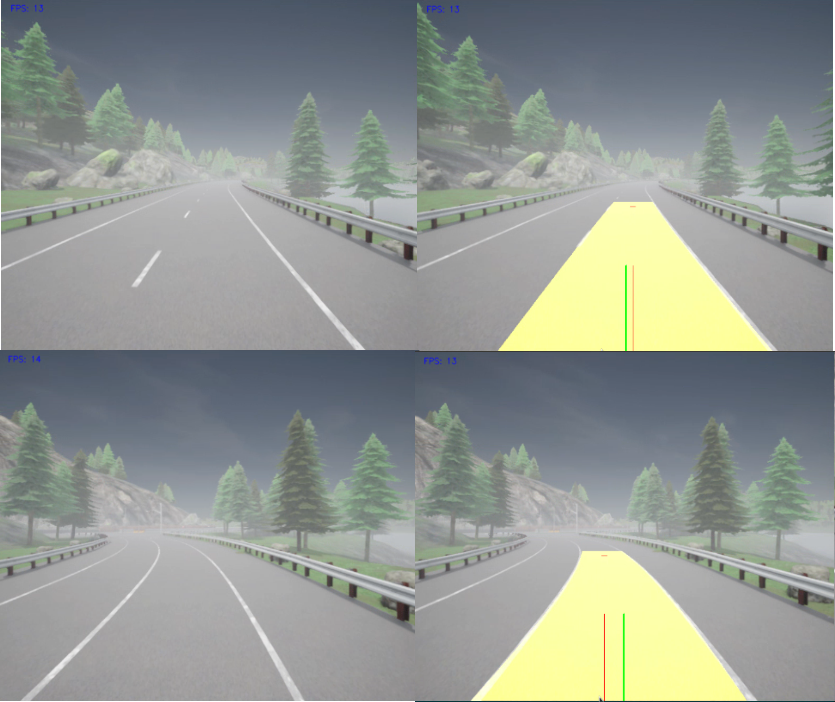
\includegraphics[height=8cm]{imagenes/cap4/graphics_sliding_window/carril_filtrado.pdf}
	\end{center}
	\caption[Carril filtrado con método de percepción sliding window]{Carril filtrado con método de percepción sliding window}
	\label{fig:Carril filtrado con método sliding window}
\end{figure}



Este tercer método de filtrado de carril esta inspirado en este proyecto \cite{sliding_window_lane_detection} realizado por Charles Wong.

\subsection{Método de percepción 4: Percepción basada en redes neuronales}
\label{Método 1: Redes neuronales}

Tras haber explorado distintos enfoques basados en visión artificial. Podemos dar paso a una nueva línea de investigación en la que se implementará y analizará un sigue carril cuya detección de carril estará basada en \ac{IA}.

\bigskip

En este método la detección de carril, la inferencia del mismo se realiza mediante una red neuronal. Más concretamente se utilizará una red neuronal convolucional \footnote{\url{https://es.wikipedia.org/wiki/Red_neuronal_convolucional}} específica para tareas de segmentación. Esta red ha sido facilitada por el grupo \textit{Roboticslaburjc} para evitar todo el proceso de entrenado de la misma el cual puede llegar a ser muy costoso temporalmente. Esta red ha sido previamente entrenada con un dataset de imágenes de distintos carriles pertenecientes a 4 mundos distintos. Esta red ha sido creada con la librería de \ac{IA} pytorch \footnote{\url{https://pytorch.org/}}. 

\bigskip

Para hacer uso de la red neuronal y lograr la detección de carriles mediante su inferencia han de seguirse una serie de pasos.

\begin{enumerate}
    \item Primero tendremos que cargar la red neuronal en nuestro programa mediante las herramientas proporcionadas por Pytorch, herramienta ya explicada en la sección \ref{subsec:PyTorch}.
    \item Posteriormente proporcionaremos las imágenes de la cámara de nuestro vehículo a la red neuronal como entrada
    \item El tercer y último paso es guardar los datos de salida de la red neuronal en los que se encuentra filtrado el carril de la imagen
\end{enumerate}

\bigskip

No obstante, al intentar probar este método nos encontramos con un problema. La limitación de recursos en la tarjeta gráfica de nuestra máquina, que estaba equipada con 6 GB de memoria, se volvió evidente al lanzar conjuntamente el simulador de conducción CARLA y el algoritmo de detección basado en redes neuronales, ya que en ese momento, se generó un error que indicaba la insuficiencia de memoria gráfica disponible para llevar a cabo estas tareas simultáneamente.

\bigskip

Para superar este obstáculo, se adoptó una estrategia que implicó realizar una pequeña modificación en la configuración. Optamos por iniciar CARLA con el flag -low-quality. Esta configuración específica tenía como resultado la disminución de la calidad visual de las imágenes generadas en el entorno virtual de CARLA. Aunque esta decisión reducía la calidad de las representaciones visuales, también se traducía en un consumo de recursos significativamente menor por parte de la tarjeta gráfica. 

\bigskip

La implementación de esta modificación demostró ser una solución efectiva para nuestro proyecto. Permitió que el algoritmo de detección basado en redes neuronales funcionara de manera adecuada y fluida

\bigskip

En esta \href{https://roboticslaburjc.github.io/2022-tfg-juancamilo-carmona/DEMOS/}{\textbf{entrada}} del blog del \ac{TFG} del blog del \ac{TFG} puede visualizar el funcionamiento de este método un video demostración. Además para una visualización más rápida en la figura \ref{fig:Carril filtrado con el método basado en una red neuronal}  también podemos encontrar una imagen donde vemos un carril filtrado por este método. Como vemos el resultado obtenido en la detección del carril es mucho mas robusto que todos los anteriores vistos. La red neuronal es capaz de filtrar el carril en todo tipo de situaciones, incluso con reflejos, cambios de luz o curvas cerradas. Solamente presenta fallos en la detección de líneas discontinuas cuando la distancia entre líneas es muy grande, sin embargo este problema podría ser fácilmente solucionado reentrenando la red neuronal, añadiendo imágenes de de carriles con este tipo de líneas discontinuas al dataset de entrenamiento.

\begin{figure} [H]
	\begin{center}
	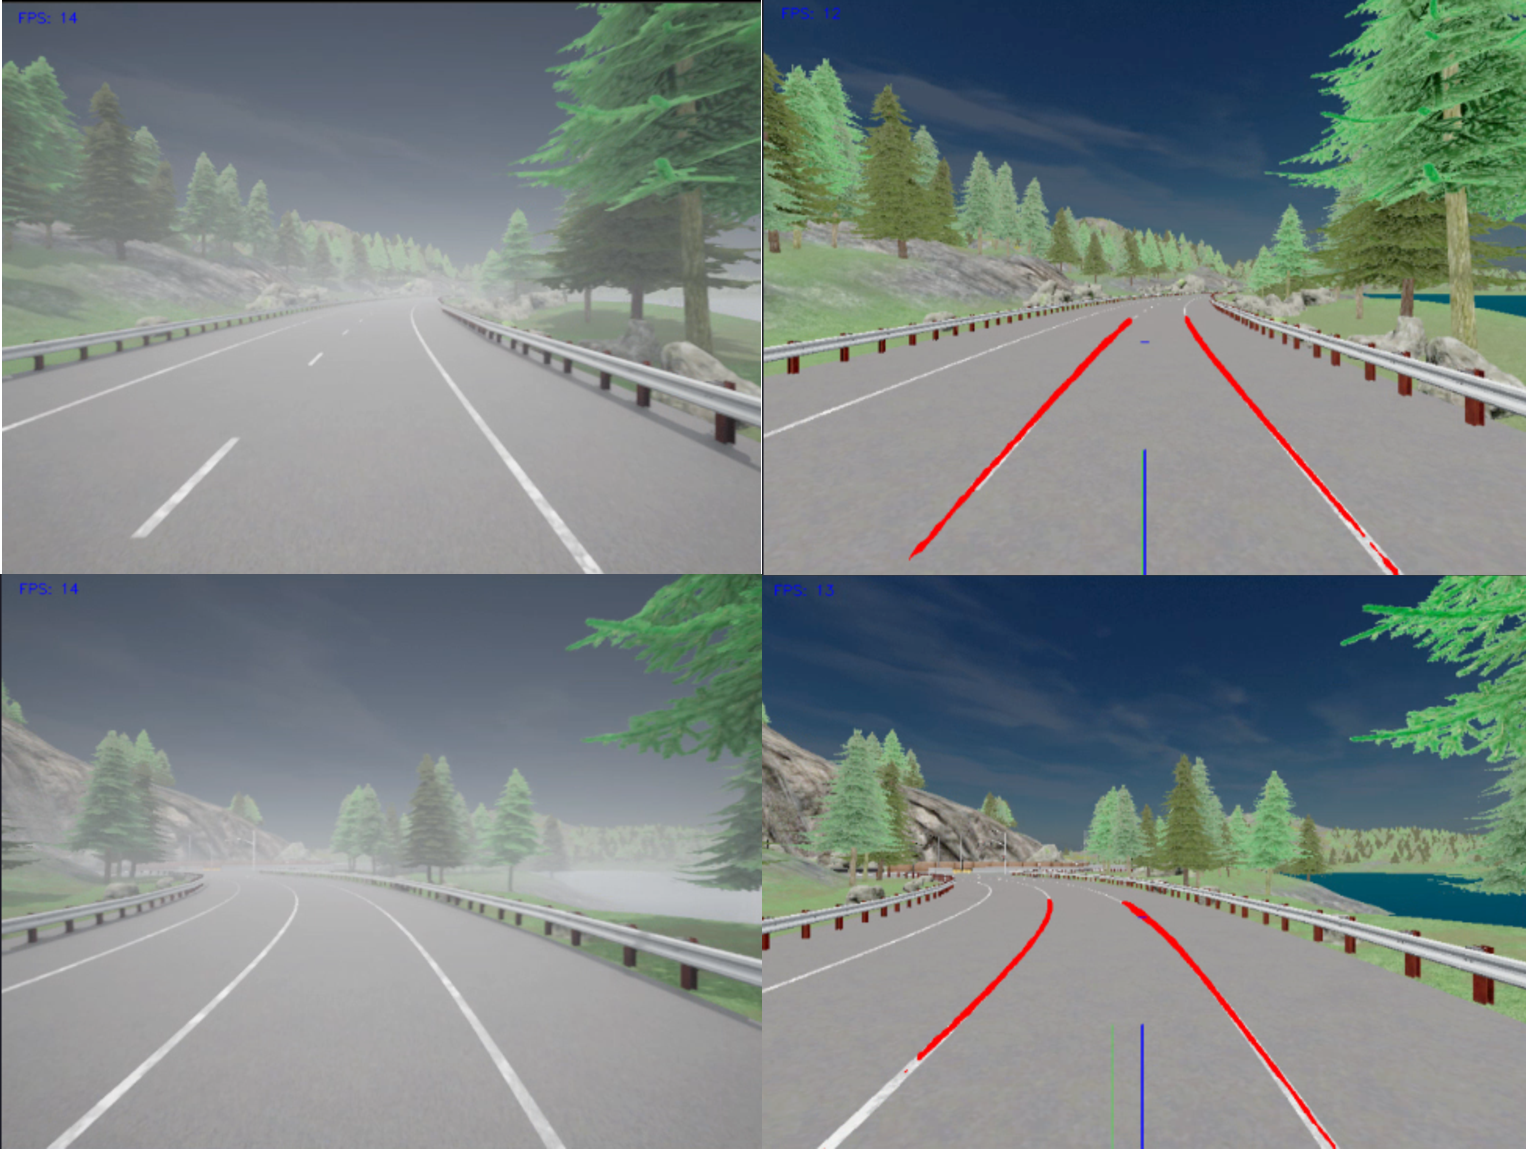
\includegraphics[height=8cm]{imagenes/cap4/graphics_deeplearning/carril_filtrado.pdf}
	\end{center}
	\caption[Carril filtrado con el método de percepción basado en una red neuronal]{Carril filtrado con el método de percepción basado en una red neuronal}
	\label{fig:Carril filtrado con el método basado en una red neuronal}
\end{figure}
\subsection{Comparación de los métodos de percepción}
\label{Comparación de los métodos de detección}

Después de exponer los resultados de los tres algoritmos basados en visión artificial y un algoritmo basado en redes neuronales, podemos llevar a cabo una comparación entre ellos para llegar a una conclusión acerca del método más eficaz en la detección de carriles. Para la obtención de los datos utilizados en estas comparaciones, todos los algoritmo se pusieron en funcionamiento en el inicio del carril derecho que se puede ver marcado con un circulo rojo en la figura \ref{fig:Circuito de pruebas} y se les permitió seguir este carril hasta llegar al final de circuito, el cual está marcado en la figura \ref{fig:Circuito de pruebas} con un circulo azul,  o se salieran del carril.

\bigskip

    \begin{figure}[h]
    \hspace{1cm}
    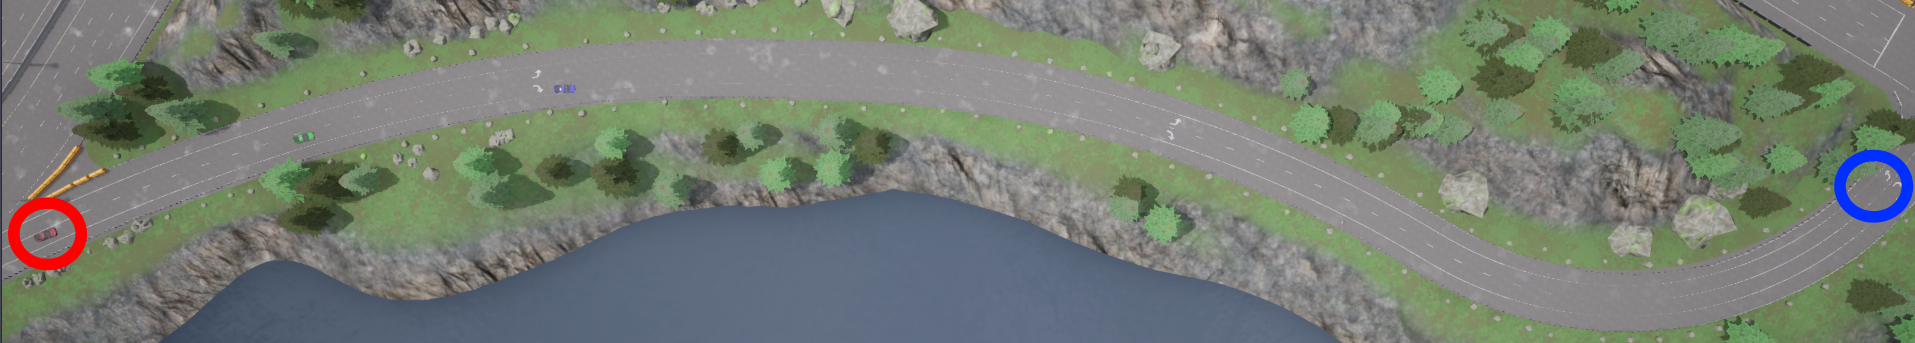
\includegraphics[height=2.5cm]{imagenes/cap4/circuito_prueba.png}
    \caption{Circuito de pruebas utilizado para la comparación de los algoritmos}
    \label{fig:Circuito de pruebas}
    \end{figure}
    
\bigskip

Primero analizaremos la tasa media de \ac{FPS} ofrecida por cada método, teniendo en cuenta que en todos los casos estamos limitados a un máximo de 15 \ac{FPS} debido al cuello de botella generado por el \textit{CARLA to ROS bridge} en la figura \ref{fig:Gráfíca de comparación de los FPS de todos los algoritmos} que los dos algoritmos más simples, que requieren menos procesamiento, logran una mayor cantidad de \ac{FPS}, acercándose significativamente al límite impuesto por el cuello de botella del ROS bridge. A continuación, se encuentra el algoritmo sliding window, que como sabemos demanda un mayor procesamiento computacional debido a esto, este algoritmo tiene la menor tasa de \ac{FPS} de todos los métodos, aún así logra mantener una tasa media aceptable de 12 \ac{FPS} por lo que el comportamiento del algoritmo sigue logrando ser fluido y reactivo. Finalmente quedaría por analizar el algoritmo basado en redes neuronales. Para este caso, es importante tener en cuenta que este algoritmo a diferencia de los demás utiliza la \ac{GPU} de la maquina en la que se ejecuta. Esto permite que a pesar ser un algoritmo pesado computacionalmente nos ofrezca una tasa media de \ac{FPS} muy alta que se acerca incluso a la de los dos algoritmos más sencillos.
\bigskip

\begin{figure}[h]
    \centering
    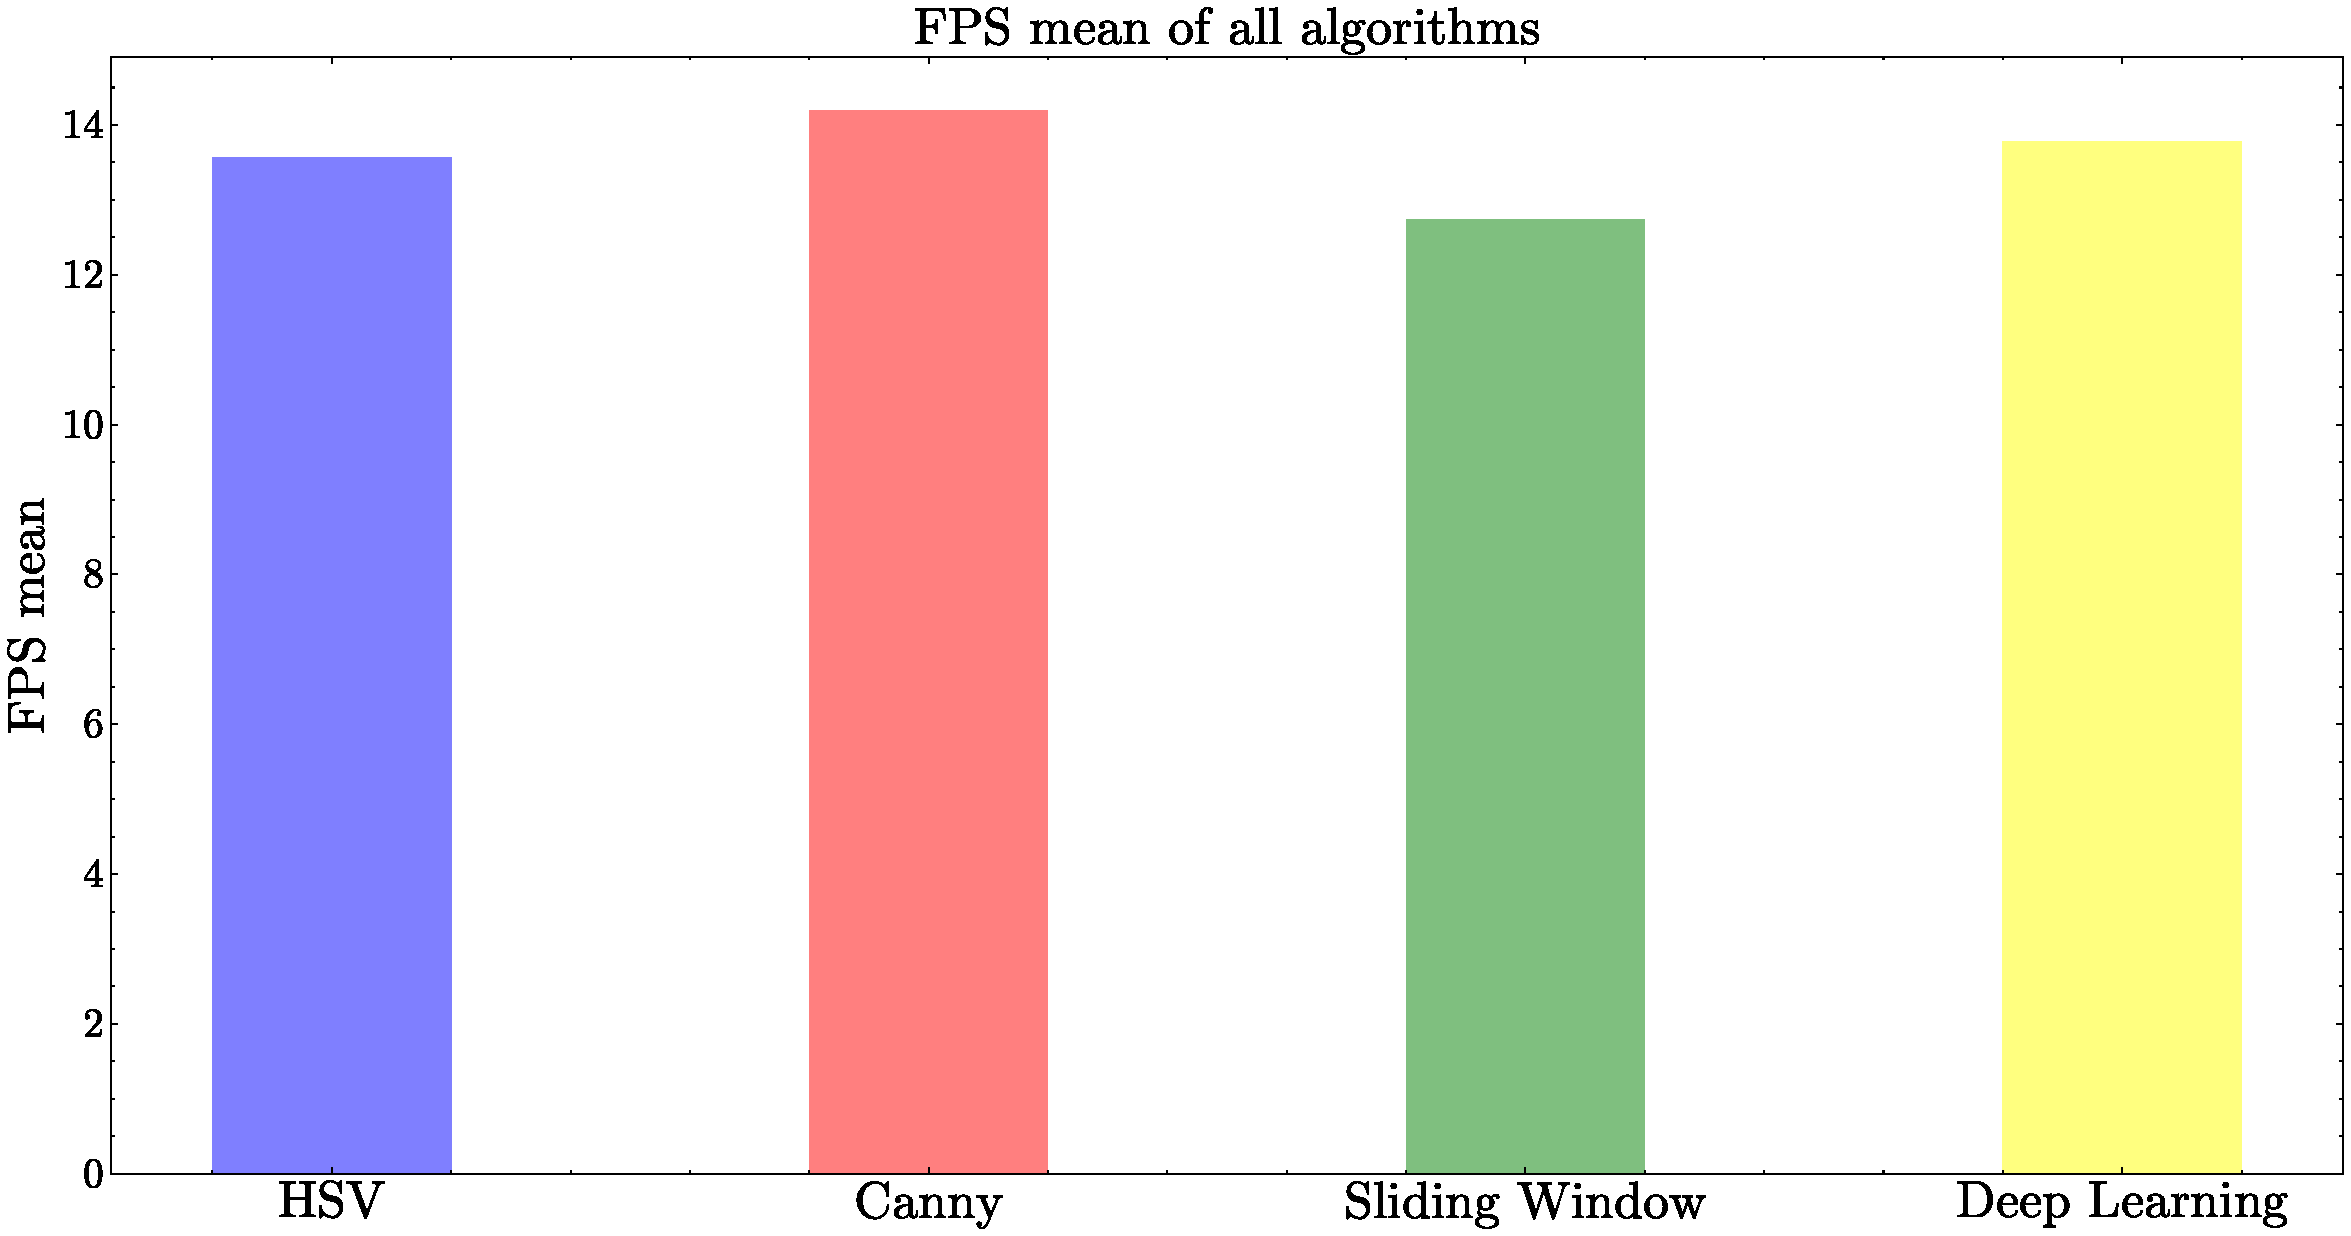
\includegraphics[height=8cm]{imagenes/cap4/graphics_comparison/fps.pdf}
    \caption{FPS medios de todos los algoritmos}
    \label{fig:Gráfíca de comparación de los FPS de todos los algoritmos}
\end{figure}
\bigskip 


Ahora analizaremos al consumo de \ac{CPU} de todos los algoritmos utilizados. En sistemas Linux, el uso de la \ac{CPU} se muestra en porcentajes y se basa en la cantidad de núcleos disponibles en la computadora. En este caso la maquina que han ejecutado todos los métodos de filtrado de carril cuenta con un sistema operativo basado en Linux por lo que para analizar el consumo de \ac{CPU} se seguirá esta nomenclatura. La maquina en la que se probaron todos estos métodos de filtrado de carril cuenta con 6 núcleos, cada núcleo se considera al 100\% de su capacidad cuando está trabajando al máximo. de manera que 600\% de uso de \ac{CPU} significaría que el algoritmo esta consumiendo todos los recursos de procesamiento de la maquina.

\bigskip
\begin{figure}[h]
    \centering
    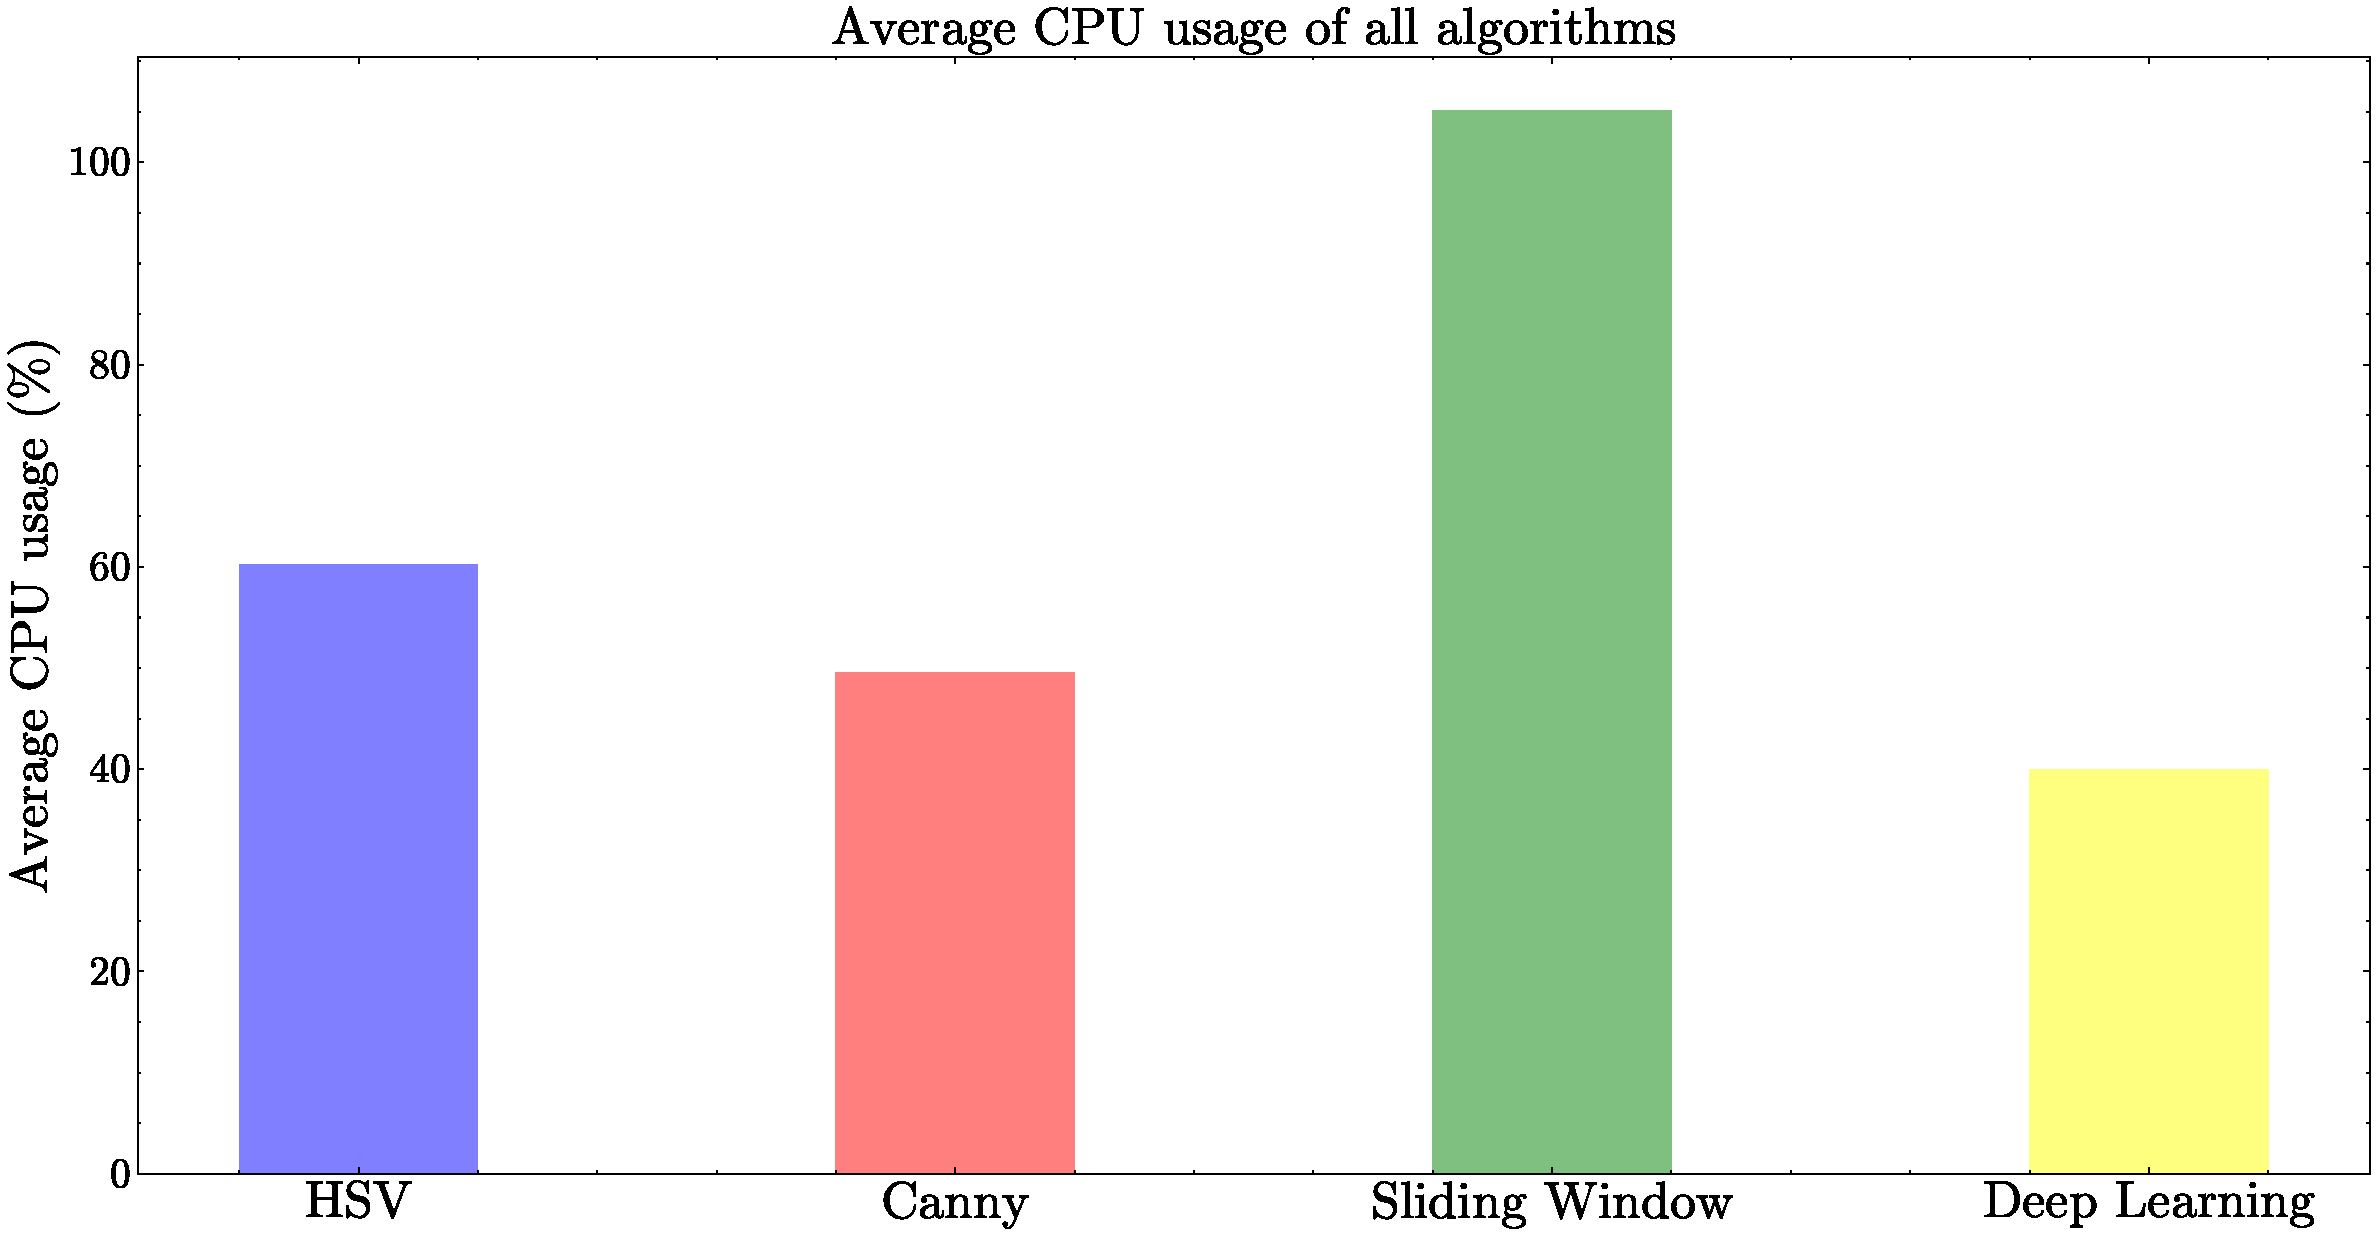
\includegraphics[height=8cm]{imagenes/cap4/graphics_comparison/cpu.pdf}
    \caption{Consumo de CPU medio de todos los algoritmos}
    \label{fig:Gráfíca de comparación del consumo de CPU de todos los algoritmos}
\end{figure}

\bigskip 

 En la figura \ref{fig:Gráfíca de comparación del consumo de CPU de todos los algoritmos}  se puede ver un histograma con el consumo medio de \ac{CPU} de todos los algoritmos. Como se ve el algoritmo basado en Canny tiene un uso medio de \ac{CPU} del 50\% esto quiere decir que el algoritmo esta necesitando tan solo la mitad de uno de los 6 núcleos del sistema para ser procesado lo cuál es lógico debido a la sencillez de este algoritmo y constituye un consumo pequeño de los recursos totales.
 
\bigskip

El método de filtrado basado en la suma de Canny y un filtro de color  HSV tampoco presenta un consumo de \ac{CPU} muy alto, para este caso, el consumo rondando ahora el 60\%. Este incremento se debe al procesamiento de imagen extra añadido a este método, sin embargo, el incremento es bastante pequeño debido a la naturaleza sencilla del mismo. 

 \bigskip
 De color verde podemos ver el consumo de \ac{CPU} del algoritmo sliding window en este caso vemos como la tasa media de consumo de \ac{CPU} se ve como es lógico incrementada superando ahora el 100\% de uso y alcanzando incluso picos del 120\%, lo que significa que nuestra maquina esta utilizando completamente uno de sus seis núcleos de procesamiento disponibles para ejecutar este algoritmo, e incluso está necesitando del uso de otro núcleo extra en ciertas ocasiones. Aquí vemos como el consumo de \ac{CPU} ha subido mucho con respecto a los anteriores algoritmos llegando incluso a duplicarlos lo que nos indica que a pesar de utilizar un algoritmo sliding window para optimizar el procesamiento, sigue siendo un algoritmo computacionalmente muy pesado.

\bigskip

Finalmente en el algoritmo basado en \ac{IA} que utiliza una red neuronal como método de detección se puede ver un consumo de \ac{CPU} que ronda el 40\%, menor que todos los demás métodos aunque sustancialmente. Sin embargo, hay que tener en cuenta que debido a la configuración establecida, en este caso particular, a pesar de que la inferencia con una red neuronal es una tarea computacionalmente muy pesada, esto no se ve reflejado en el consumo de \ac{CPU} del sistema debido a que el procesamiento de imágenes por parte de la red neuronal se realizaba utilizando la \ac{GPU}, esto es una ventaja ya que permite liberar de trabajo de procesamiento gráfico a la \ac{CPU}, delegándoselo a la \ac{GPU} la cuál está especialmente diseñada para ello.

\bigskip

La siguiente comparación que se va a presentar se puede observar en la figura \ref{fig:Gráfica de ruta seguida por todos los algoritmos} aquí se puede observar distintas gráficas de diferentes tramos de la  ruta que han seguido los distintos algoritmos mostrada antes en la figura \ref{fig:Circuito de pruebas}. En general todos los algoritmos consiguen filtrar el carril de manera efectiva y seguir el mismo durante el recorrido entero. Sin embargo existen diferencias sutiles en los trayectos de cada algoritmo. Como se comento anteriormente todos los algoritmos utilizan el mismo controlador \ac{PID} para controlar el manejo del vehículo, por lo que la variación en la ruta estará enteramente dictado por la percepción. Los algoritmos más sencillos, como el método de Canny y la combinación de Canny con HSV, tienden a trazar las curvas de manera más cerrada y abrupta. Por otro lado, los algoritmos más complejos y robustos generalmente describen las curvas de una manera más abierta y natural, lo cual podría ser preferible en aplicaciones donde se busca una conducción más suave y segura.

\bigskip

\begin{figure}[h]
    \centering
    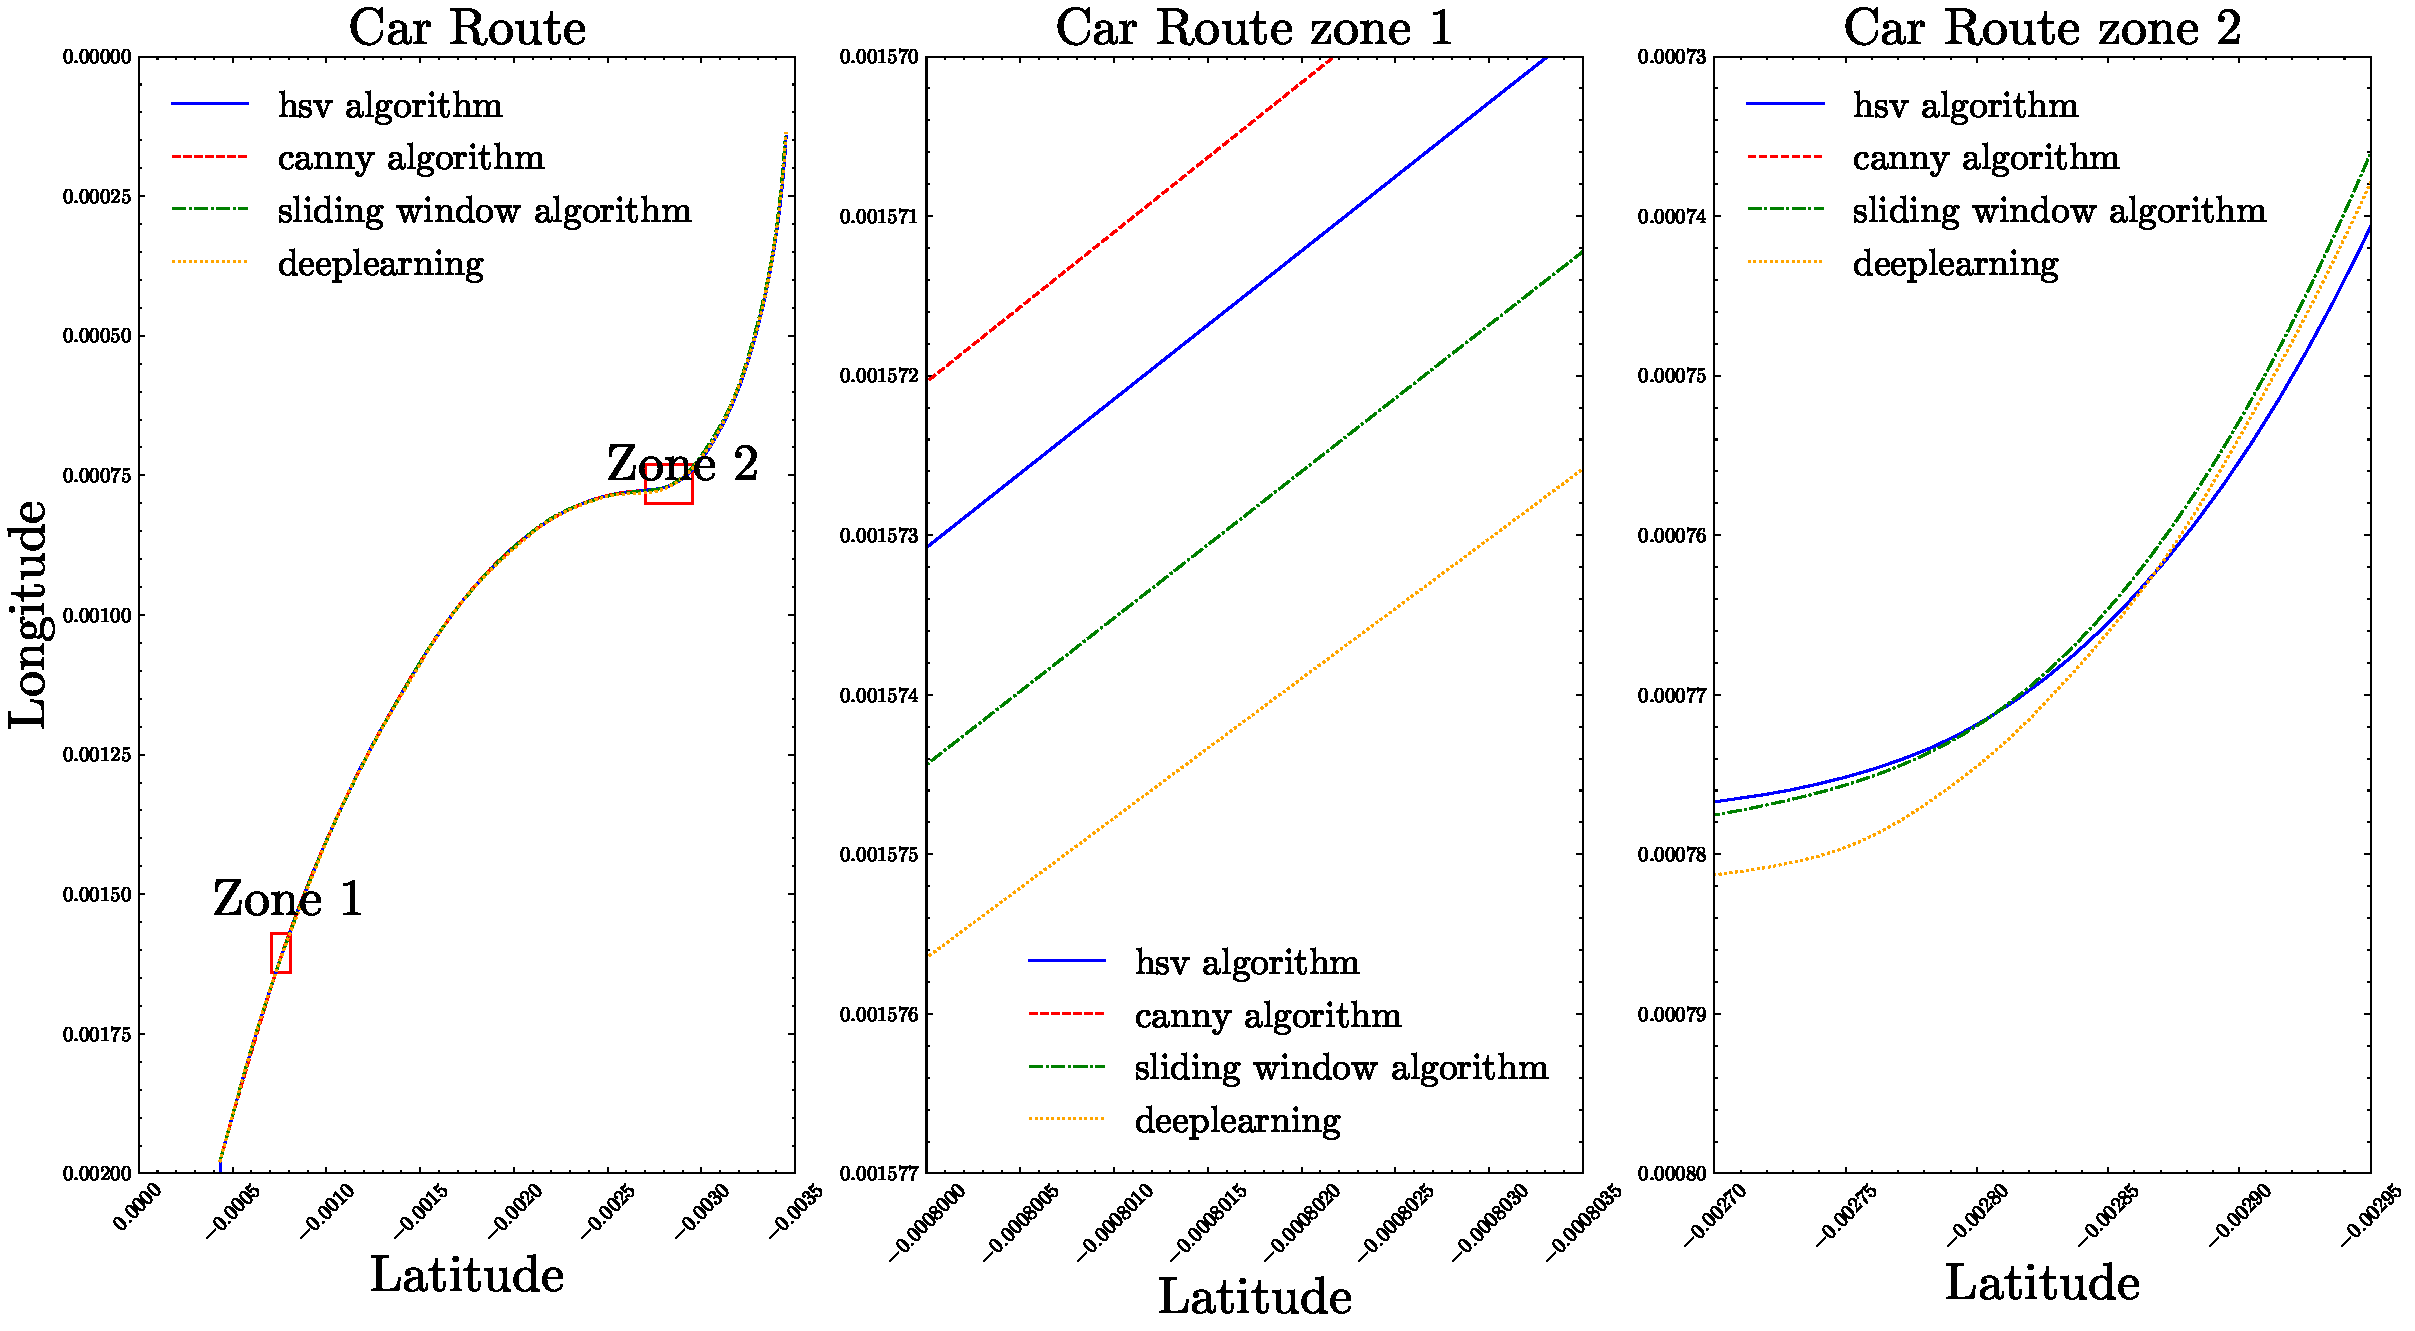
\includegraphics[height=8cm]{imagenes/cap4/graphics_comparison/route.pdf}
    \caption{Gráfica de ruta seguida por todos los algoritmos}
    \label{fig:Gráfica de ruta seguida por todos los algoritmos}
\end{figure}

\bigskip

Si miramos la gráfica de la figura \ref{fig:Gráfica de los tipos movimientos de los PID de todos los algorimtos} en donde se muestra que movimientos realiza cada algoritmo ( giros a la izquierda, a la derecha y ausencia de giros) vemos como en los métodos más complejos y especialmente en el algoritmo de detección basado en redes neuronales, realizan un menor porcentaje de acciones de giros, manteniendo al vehículo durante más tiempo recto sin tener que corregir su posición \ref{fig:Gráfica de los tipos movimientos de los PID de todos los algorimtos}, esto es una gran ventaja ya que favorece una conducción menos oscilatoria y mas fluida, además por otro lado si observamos la gráfica ECDF en la que se presenta la intensidad de los giros realizados por cada algoritmo \ref{fig:Gráfica de la función ECDF de la insensidad de los giros de cada algoritmo},  podemos contrastar lo visto en la grafica \ref{fig:Gráfica de los tipos movimientos de los PID de todos los algorimtos} ya que nuevamente vemos como el algoritmo con percepción basada en redes neuronales tiene un mayor porcentaje de giros nulos, es decir de mantener el volante recto y no realizar ningún giro en absoluto en adición a esto,tambíen podemos observar que  los giros que si realiza son menos  intensos que en los demás casos ya que podemos notar como la gráfica de este algoritmo crece manera mucha mas suave y paulatina que la de los los demás métodos. Lo que podemos concluir de esta información es que debido a la mejora de percepción en el algoritmo de filtrado basado en una red neuronal el controlador \ac{PID} tiene una mayor exactitud al mantenerse el centro del carril y en consecuencia tiene que realizar una menor cantidad de giros con menos intensidad para corregir la trayectoria y seguir el carril lo cuál resulta en una conducción más suave y fluida.

\begin{figure}[t]
    \centering.
    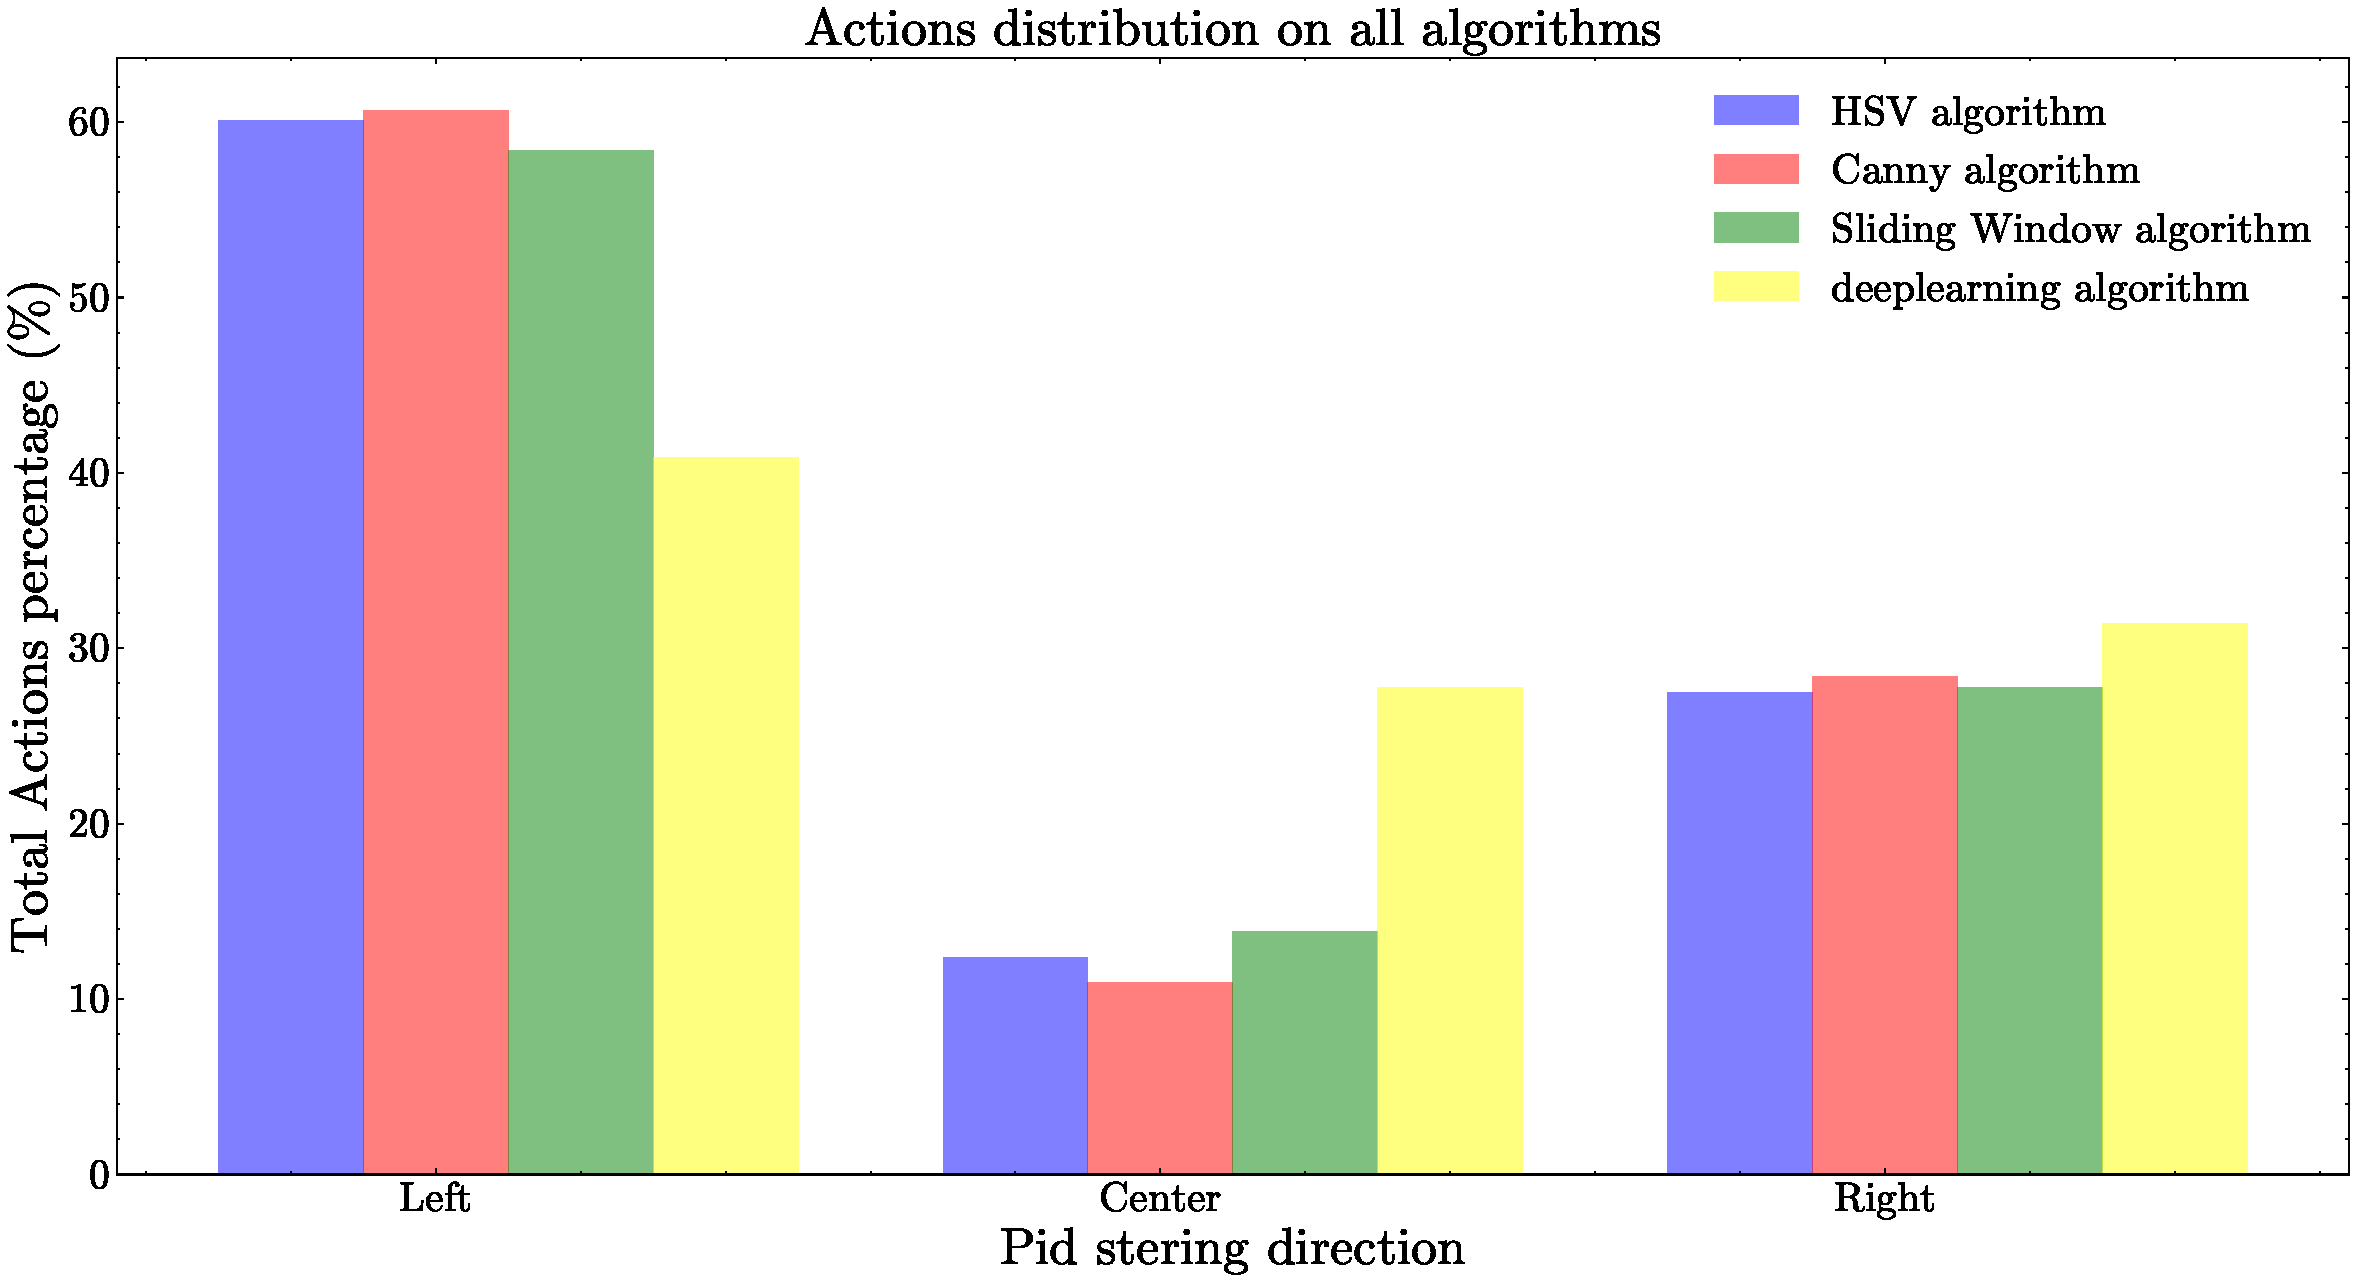
\includegraphics[height=8cm]{imagenes/cap4/graphics_comparison/pid_curling.pdf}
    \caption{Gráfica de los tipos movimientos de los PID de todos los algorimtos}
    \label{fig:Gráfica de los tipos movimientos de los PID de todos los algorimtos}
\end{figure}

\begin{figure}[t]
    \centering
    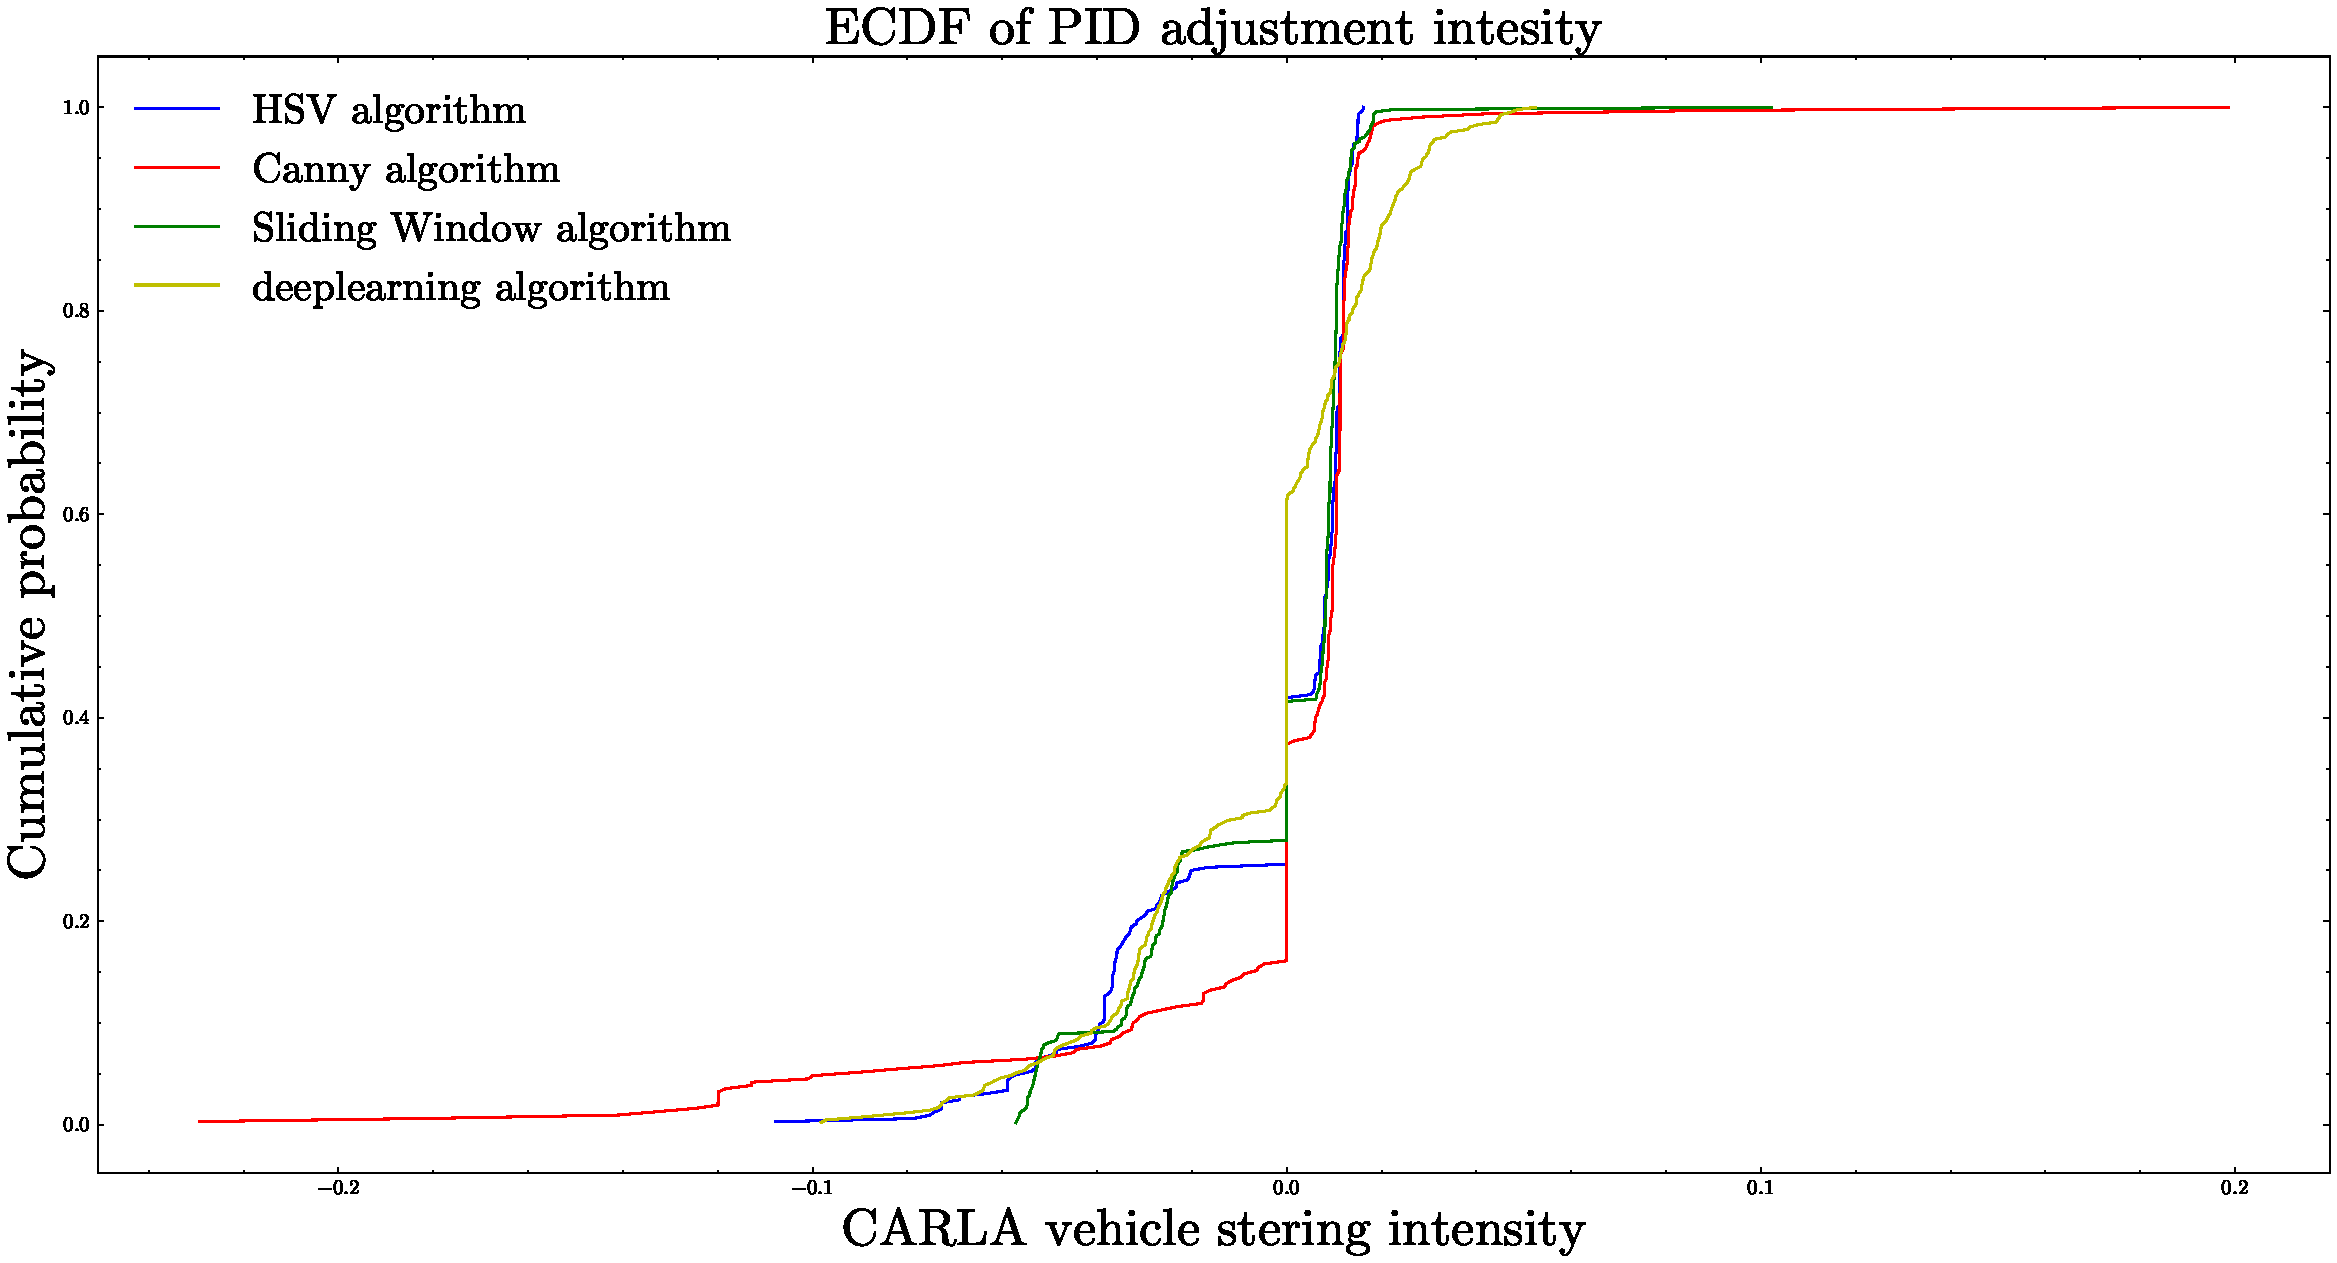
\includegraphics[height=8cm]{imagenes/cap4/graphics_comparison/ECDF.pdf}
    \caption{Gráfica de la función ECDF de la insensidad de los giros de cada algoritmo}
    \label{fig:Gráfica de la función ECDF de la insensidad de los giros de cada algoritmo}
\end{figure}


\bigskip

En términos generales, todos los algoritmos que hemos desarrollado logran, en su medida, filtrar el carril de manera lo suficientemente efectiva como para realizar un seguimiento del mismo. Sin embargo, aunque para nuestro caso concreto y en condiciones ideales los algoritmos sustentados por métodos más sencillos, como lo son el algoritmo basado en el filtro Canny y el algoritmo basado en filtro Canny + filtro de color HSV, resulten eficaces tienen una enorme vulnerabilidad ante cambios de luz, sombras y brillos, esto genera que no sean algoritmos robustos ni generalistas que puedan funcionar de manera adecuada en un entorno real. Por otro lado,los algoritmos más complejos como el pipeline de filtrado con Sliding Window y el que utiliza una red neuronal como método de detección demuestran una mayor robustez, siendo capaces de operar eficazmente en un rango más amplio de escenarios. 

\bigskip

Además de esto, el algoritmo basado en Redes Neuronales ofrece una tasa de cuadros por segundo \ac{FPS} más alta, debido a una inferencia más rápida y al más adecuado aprovechamiento de los recursos del sistema ofreciéndonos la opción de utilizar la \ac{GPU} de la maquina para realizar el procesamiento de las imágenes, en este caso nos encontramos limitados por el ROS bridge, pero en pruebas realizadas en el servidor Landau de la Escuela de ingeniería superior de Fuenlabrada de la \ac{URJC} se alcanzan incluso tasas de hasta 100 \ac{FPS}. Debido a la mejora de inferencia este algoritmo nos ofrece una mayor reactividad en la toma de decisiones del vehículo. Este método de detección por otro lado, también ofrece la flexibilidad de reentrenar la red neuronal para adaptarse a nuevos escenarios para los cuales actualmente no este preparado o para mejorar su rendimiento, sin la necesidad de modificar el código fuente. Esta es una ventaja significativa sobre el algoritmo de sliding window, donde cualquier mejora en de la aplicación requeriría una revisión y modificación sustancial del código. Por estos motivos y con los argumentos presentados se ha elegido el método de inferencia de carril basada en redes neuronales, como el método de filtrado estándar para las implementaciones finales de este \ac{TFG}

\bigskip

\section{Sigue carril basado en redes neuronales y Q-learning}
\label{Sigue carriles basado en redes neuronales y Qlearnig}

\subsection{Evaluación de la Compatibilidad entre ROS 2 y CARLA a través del CARLA to ROS Bridge}
\label{Evaluación de la Compatibilidad entre ROS y CARLA a través de ROS Bridge}

Tras realizar probar distintos algoritmos utilizando ROS 2 y CARLA mediante el uso de ROS bridge, podemos concluir que la posibilidad de controlar CARLA a través de los métodos y \textit{topics} que ofrece ROS 2,  representa una herramienta sumamente útil. Este enfoque abre un amplio abanico de posibilidades para el desarrollo de nuevas aplicaciones dentro de este sistema operativo, las cuales pueden ser probadas en un entorno simulado tan realista como el que ofrece CARLA. Sin embargo, actualmente con la limitación de la tasa \ac{FPS} impuesta por el cuello de botella que produce \textit{CARLA to ROS bridge} trabajar de manera profesional con estos dos entornos todavía no es posible. desarrollar aplicaciones de conducción autónoma con un máximo de 15 \ac{FPS} en las imágenes que recibimos, aunque puede ser suficiente para la creación de prototipos, pero resulta insuficiente para aplicaciones más robustas y completas.

\bigskip
Debido a esta restricción, se ha decidido que para las implementaciones finales de este \ac{TFG} no se utilizará ROS bridge. En su lugar, se migrará todo el código necesario para continuar con el desarrollo de las aplicaciones finales a la \ac{API} nativa de CARLA en Python.

\bigskip

Esta decisión resulto ser muy acertada, pues tras la migración de ROS 2 a la \ac{API} de CARLA la tasa máxima de \ac{FPS} que se alcanzaba con el método de detección de carril basado en una red neuronal, se incremento significativamente ofreciendo ejecuciones de alrededor de 25 \ac{FPS}

\subsection{Sigue carril basado en Q-learning}
\label{Sigue carril}

Tras la imposición de la red neuronal como el mejor método para la detección de carriles, se ha consolidado su papel central como método de filtrado en las implementaciones finales de los sistemas de seguimiento de carriles. El siguiente paso gira en torno a seleccionar un método para controlar el manejo del vehículo. Hasta este momento, se había empleado un controlador \ac{PID}, el cuál constituye un enfoque tradicional y que funciona muy bien cuando se adapta específicamente a una tarea o un entorno determinado. No obstante, para ofrecer una solución final más generalista y robusta, para los diseños de los sigue carril finales con funcionalidades más complejas se utilizará una aproximación más innovadora basada nuevamente en \ac{IA}. En particular se ha optado por un algoritmo de aprendizaje por refuerzo, más concretamente, se ha implementado una variante propia de un algoritmo Q-learning para controlar el manejo del vehículo.

\bigskip


Como se detalló en la sección \ref{Método 1: Redes neuronales}, la máquina en la que se venía ejecutando los algoritmos presentados hasta ahora, mostró ciertas limitaciones, en lo que respecta a la potencia gráfica. Esto se manifestó como una incapacidad para ejecutar de manera óptima la simulación en CARLA junto con el algoritmo de detección de carriles basado en redes neuronales al mismo tiempo.

\bigskip

Dadas estas limitaciones, se ha decidido trasladar el desarrollo, entrenamiento e implementación de los algoritmos que ahora se van a desarrollar al servidor Landau explicado con más detalle en la  sección \ref{subsec:Servidor landau de la URJC}. En este entorno, la capacidad gráfica no representa una barrera, permitiendo así una implementación más ágil y eficiente de los distintos componentes del proyecto.

\bigskip

Al implementar el algoritmo de Q-learning para el seguimiento de carriles, es esencial definir sus componentes fundamentales. En este contexto, identificamos los siguientes elementos clave:
\bigskip


\begin{itemize}
    \item \textbf{Estados:} Para esta implementación, dividimos verticalmente la imagen de la cámara en múltiples franjas. Cada una de estas franjas representa un estado del algoritmo de Q-learning. Hay 11 franjas separadas equidistantemente por 20 pixeles empezando en el centro de la imagen y extendiéndose a cada lado, luego hay dos ultimas franjas desde donde terminan estas 11 iniciales hasta el resto de la imagen, esto resulta en un total de 24 estados tal y como se ve en la figura \ref{fig:Estados del algoritmo de Q-learnig}. La determinación del estado actual se basa en las coordenadas de píxeles en los que se encuentra ubicado el centro del carril detectado.
  
  \begin{figure}[h]
    \centering
    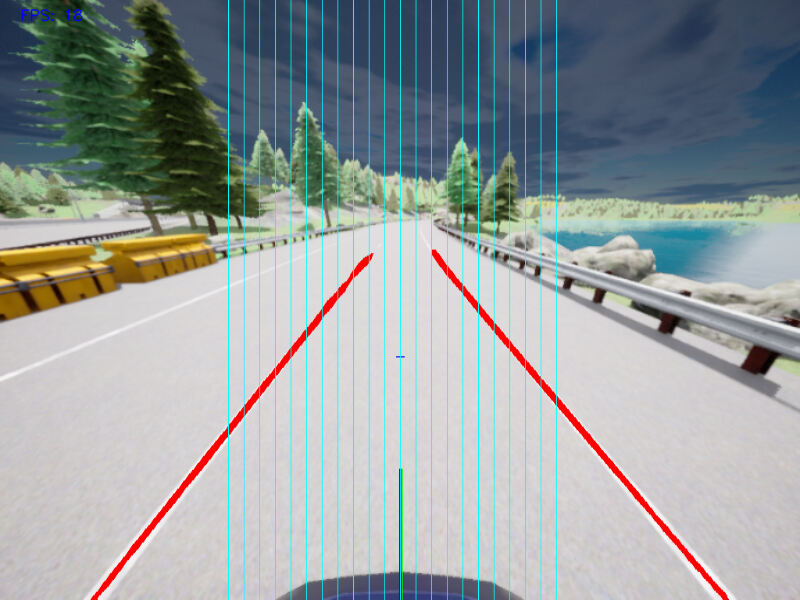
\includegraphics[height=8cm]{imagenes/cap4/estados_qlearnig.png}
    \caption{Estados del sigue carril basado en Q-learnig}
    \label{fig:Estados del algoritmo de Q-learnig}
\end{figure}
    
    \newpage 
    
    \item \textbf{Agente:} Es el componente que realiza las acciones e interactúa con el entorno, en este contexto el agente es el vehículo que realiza el seguimiento de carril.
    
    \item \textbf{Acciones:} Se han definido una serie de acciones que el agente puede llevar a cabo. Primero tenemos las acciones de giros de dirección, donde especificamos la cantidad de rotación que se aplica al volante del vehículo. Hemos considerado 9 acciones para girar a la derecha, 9 acciones para girar a la izquierda y una acción de giro nulo, lo que suma un total de 19 acciones relacionadas con el control de la dirección. Además, hemos incorporado acciones relacionadas con la velocidad lineal, definiendo 4 velocidades lineales distintas. Estas acciones permiten regular la velocidad del vehículo a medida que avanza por el circuito. En código \ref{cod:Acciones disponibles para el algoritmo de qlearning} podemos ver la implementación de las acciones definidas junto con sus valores para este caso. El giro del volante esta normalizado entre -1 y 1 de manera que -1 equivale a girar el volante completamente a la izquierda, +1 equivale a girar el volante completamente a la derecha y 0 a mantener el volante en el centro
    \bigskip
    \begin{code}[H]
	\begin{lstlisting}[language=Python]
        self.ACTIONS = [ 
            'forward',   #stering = -0.0
            'left_1',    #stering = -0.02     
            'left_2',    #stering = -0.04
            'left_3',    #stering = -0.06
            'left_4',    #stering = -0.08
            'left_5',    #stering = -0.1
            'left_6',    #stering = -0.12
            'left_7',    #stering = -0.14
            'left_8',    #stering = -0.16  
            'left_9',    #stering = -0.18 
            'right_1',   #stering = 0.02  
            'right_2',   #stering = 0.04
            'right_3',   #stering = 0.06  
            'right_4',   #stering = 0.08     
            'right_5',   #stering = 0.1 
            'right_6',   #stering = 0.12 
            'right_7',   #stering = 0.14 
            'right_8',   #stering = 0.16 
            'right_9',   #stering = 0.18
        ]
        self.SPEED = [ 
            'speed_1',   #stering = 3.5 m/s  
            'speed_2',   #stering = 4.0 m/s  
            'speed_3',   #stering = 4.5 m/s
            'speed_4'    #stering = 5.0 m/2        ]
	\end{lstlisting}
\caption[Acciones disponibles para el sigue carril basado en Q-learning]{Acciones disponibles para el sigue carril basado en Q-learning}
\label{cod:Acciones disponibles para el algoritmo de qlearning}
\end{code}
    
    
    \item \textbf{Entorno:} El entorno es el componente de un algoritmo de Q-learning donde el agente toma decisiones y ajusta su comportamiento en función de las acciones al estado actual y a la función recompensa. El entorno utilizado para el entrenamiento de este algoritmo es el mismo circuito que hemos estado utilizando en las pruebas de los demás algoritmos del \ac{TFG}.
    \begin{figure}[H]
    \hspace{1cm}
    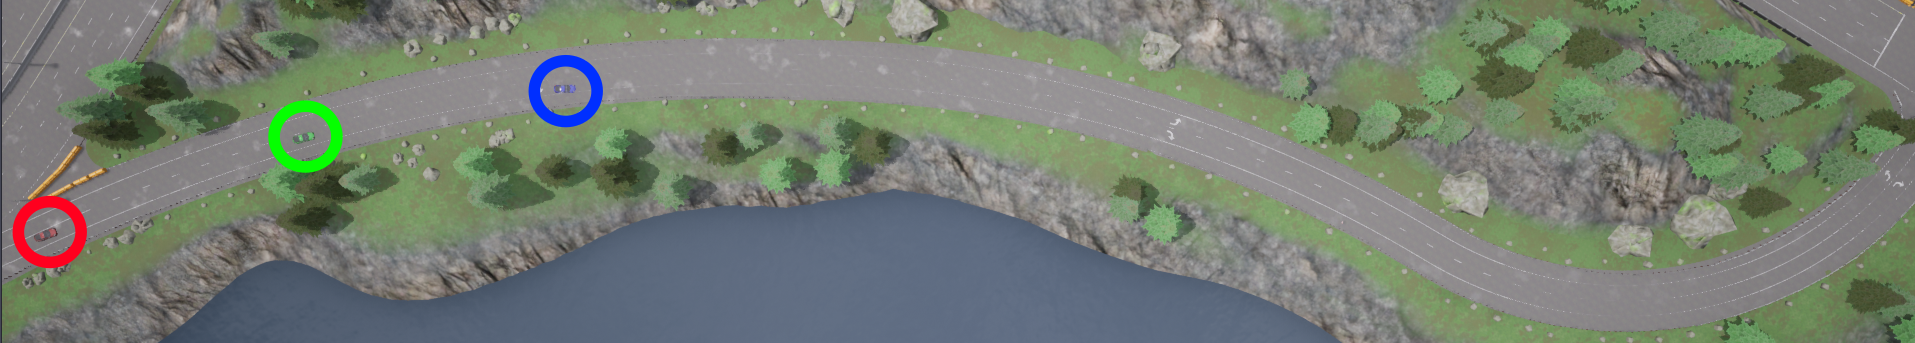
\includegraphics[height=2.5cm]{imagenes/cap4/entorno_qlearnig.png}
    \caption{Entorno de entrenamiento del sigue carril basado en Q-learnig}
    \label{fig:Entorno de entrenamiento del algoritmo de Q-learnig}
    \end{figure}
    
     Dentro de este circuito además se han elegido tres puntos distintos para generar el vehículo a la hora de realizar el entrenamiento de Q-learning, estas localizaciones estan marcada con un circulo cada uno de un color distinto en la figura \ref{fig:Entorno de entrenamiento del algoritmo de Q-learnig}. Estas localizaciones además de el propio circuito se pueden ver en la figura \ref{fig:Entorno de entrenamiento del algoritmo de Q-learnig}.
    
    \bigskip    
    \item \textbf{Función de Recompensa:} La función de recompensa desempeña un papel fundamental en la adaptación del comportamiento del vehículo. En esta implementación, la función de recompensa se diseña para premiar velocidades lineales rápidas, lo que impulsa al vehículo a mantener la velocidad media más alta posible. Además, se recompensa al vehículo por mantener el centro del carril alineado con el centro de la imagen, lo que garantiza que el vehículo se mantenga en una posición central en la carretera y además también se premia al vehículo por mantener un ángulo adecuado con respecto al carril, asegurando que se conduzca de manera paralela al mismo. La implementación de la función recompensa puede verse en el código \ref{cod:Función recompensa del algoritmo de qlearning}.
   
    \bigskip
\begin{code}[H]
	\begin{lstlisting}[language=Python]	
    def reward_function(self, error, angle_error,car_crashed):

        if self.lane_lines < 1:
            reward = 0.0
            return reward
            
        if car_crashed:
            reward = 0.0
            return reward

        normalized_error = abs(error)
       #calculate the reward based on the lanes center location
       # our speed and the angle with the road
        reward = ((((1 / (normalized_error + 1)) + self.speed/100) - angle_error/100))
        reward = np.clip(reward, -1.0, 1.0)
        reward = 1 / (1 + np.exp(-reward))

        return reward
	\end{lstlisting}
\caption[Función recompensa del sigue carril basado en de Q-learning]{Función recompensa del sigue carril basado en Q-learning}
\label{cod:Función recompensa del algoritmo de qlearning}
\end{code}
 
 \bigskip
 
 \item \textbf{Parámetros y fórmula de Q-learning:} Finalmente, el último componente del algoritmo de Q-learning que nos queda por mencionar es la fórmula propia del algoritmo y los parámetros que la componen. La fórmula de Q-learning define la política con la que vamos a rellenar la tabla Q; en este caso, se ha utilizado el enfoque \textit{Greedy}\footnote{\url{https://www.baeldung.com/cs/epsilon-greedy-q-learning}}. Este enfoque favorece siempre las recompensas máximas y tiene la siguiente fórmula. \begin{equation}Q(s, a) \leftarrow (1-\alpha) \cdot Q(s, a) + \alpha \cdot \left( r + \gamma \cdot \max_{a'} Q(s', a') \right)\end{equation} En cuanto a los parámetros que la componen, se optó por un ratio de aprendizaje (\(\alpha\)) de 0.5 para permitir un equilibrio en la incorporación de nuevas recompensas y conocimientos previos. El factor de descuento (\(\gamma\)) se estableció en 0.95 para dar importancia a las recompensas futuras en una secuencia de decisiones. Además, se inicia el entrenamiento con un ratio de exploración (\(\epsilon\)) de 0.95 que se reducía en 0.1 cada cierto número de episodios hasta llegar a 0, momento en el cual cuando se establece un valor fijo muy pequeño sin llegar a ser cero para el resto del entrenamiento, como se puede observar en la figura \ref{fig:Evolución del ratio de exploración del algoritmo Qlearnig}. Esto se realizaba con el objetivo de explorar ampliamente el espacio de estados al principio y posteriormente enfocarse en explotar lo aprendido, aunque sin cerrar completamente la ventana de seguir aprendiendo.
      
\bigskip

Una vez acabada la implementación del algoritmo, la siguiente fase era entrenarlo, la metodología para esta fase consistía en dejar entrenando el algoritmo de Q-learning en el servidor Landau de la \ac{URJC}, ya explicado en la sección \ref{subsec:Servidor landau de la URJC}, durante periodos que oscilaban entre las 6 y las 12 horas aproximadamente. De esta manera nos aseguramos que el algoritmo realizará un entrenamiento completo y acabará convergiendo. En las figuras \ref{fig:Evolución del ratio de exploración del algoritmo Qlearnig} y \ref{fig:Evolución de la recompensa acumulada del algoritmo del sigue carriles basado en Qlearnig} se presentan dos gráficas con información para analizar el entrenamiento del programa.

\bigskip

  \begin{figure}[h]
    \centering
    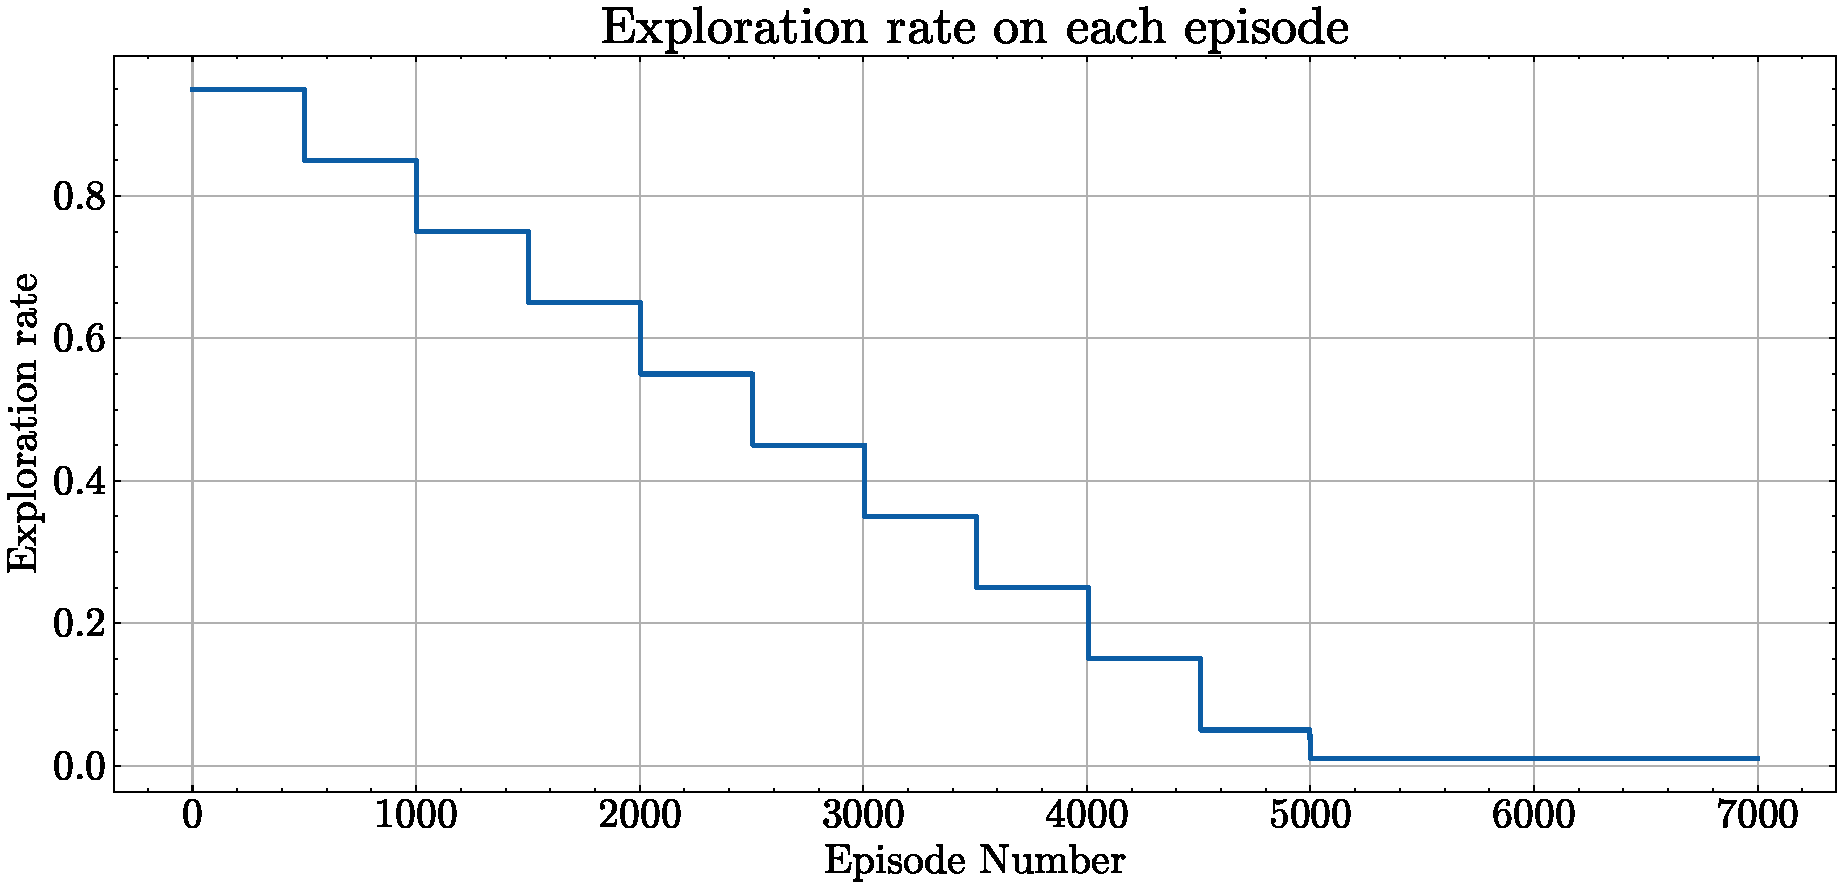
\includegraphics[height=6cm]{imagenes/cap4/sigue_carriles_qlearning/exploration_rate.pdf}
    \caption{Evolución del ratio de exploración del sigue carril basado en Q-learnig}
    \label{fig:Evolución del ratio de exploración del algoritmo Qlearnig}
\end{figure}
        
\end{itemize}

  \begin{figure}[h]
    \centering
    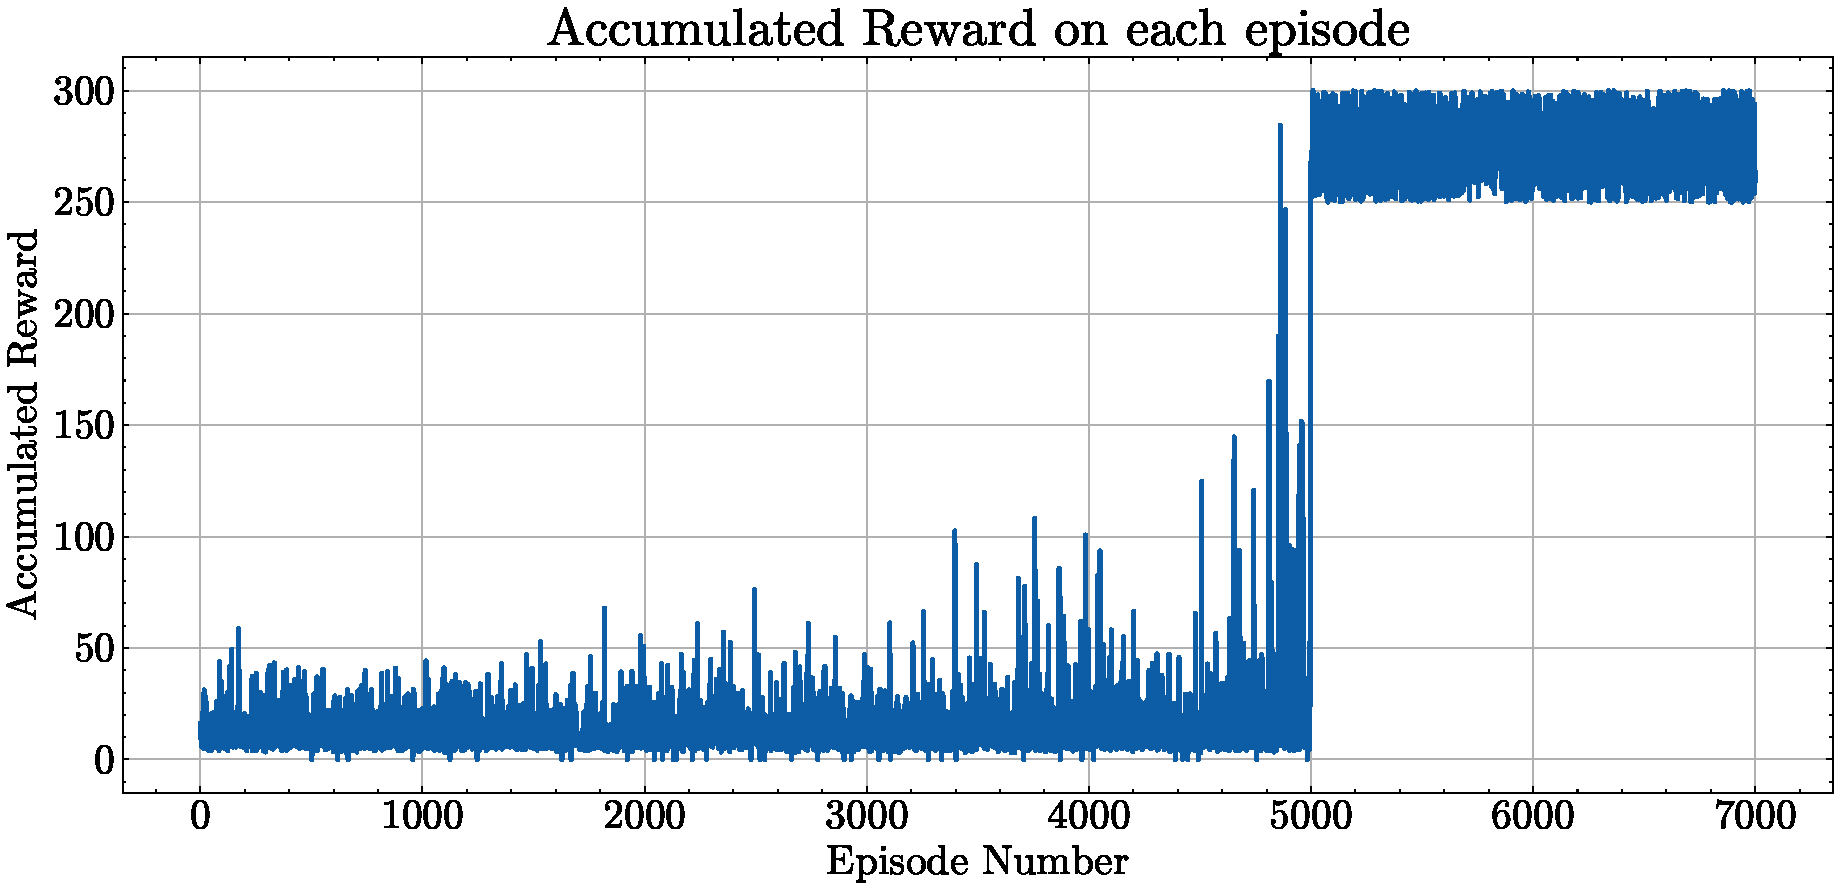
\includegraphics[height=6cm]{imagenes/cap4/sigue_carriles_qlearning/recompense.pdf}
    \caption{Evolución de la recompensa acumulada del sigue carril basado en Q-learnig}
    \label{fig:Evolución de la recompensa acumulada del algoritmo del sigue carriles basado en Qlearnig}
\end{figure}
Como vemos en las gráficas el algoritmo converge, a partir de los 5000 episodios, cuanto el ratio de exploración se vuelve muy pequeño. La convergencia se presenta en una franja de ente las 250 y las 300 unidades de recompensa y no siempre a una recompensa concreta como suele suceder en algoritmos de Q-learning. Esto no significa que el algoritmo no converja adecuadamente o que haya entrenado mal, ya que este fenómeno se debe al hecho de que este algoritmo ha sido entrenado en un circuito lineal como se puede ver en la figura \ref{fig:Entorno de entrenamiento del algoritmo de Q-learnig} donde el agente comienza cada episodio en uno de los tres sitios seleccionados, sin embargo siempre termina al finalizar la carretera. Esto lo que genera es que en los episodios donde el agente empieza más alejado de la meta al tener que recorrer más camino la recompensa que se acumula es mayor y en los episodios en los que el agente empieza más cerca del final del circuito al recorrer menos espacio la recompensa es menor. Dándonos como resultado una gráfica en la que a pesar que vemos que el algoritmo converge, éste lo hace en una franja amplia de valores dependiendo de donde comience el episodio.


  \begin{figure}[H]
    \centering
    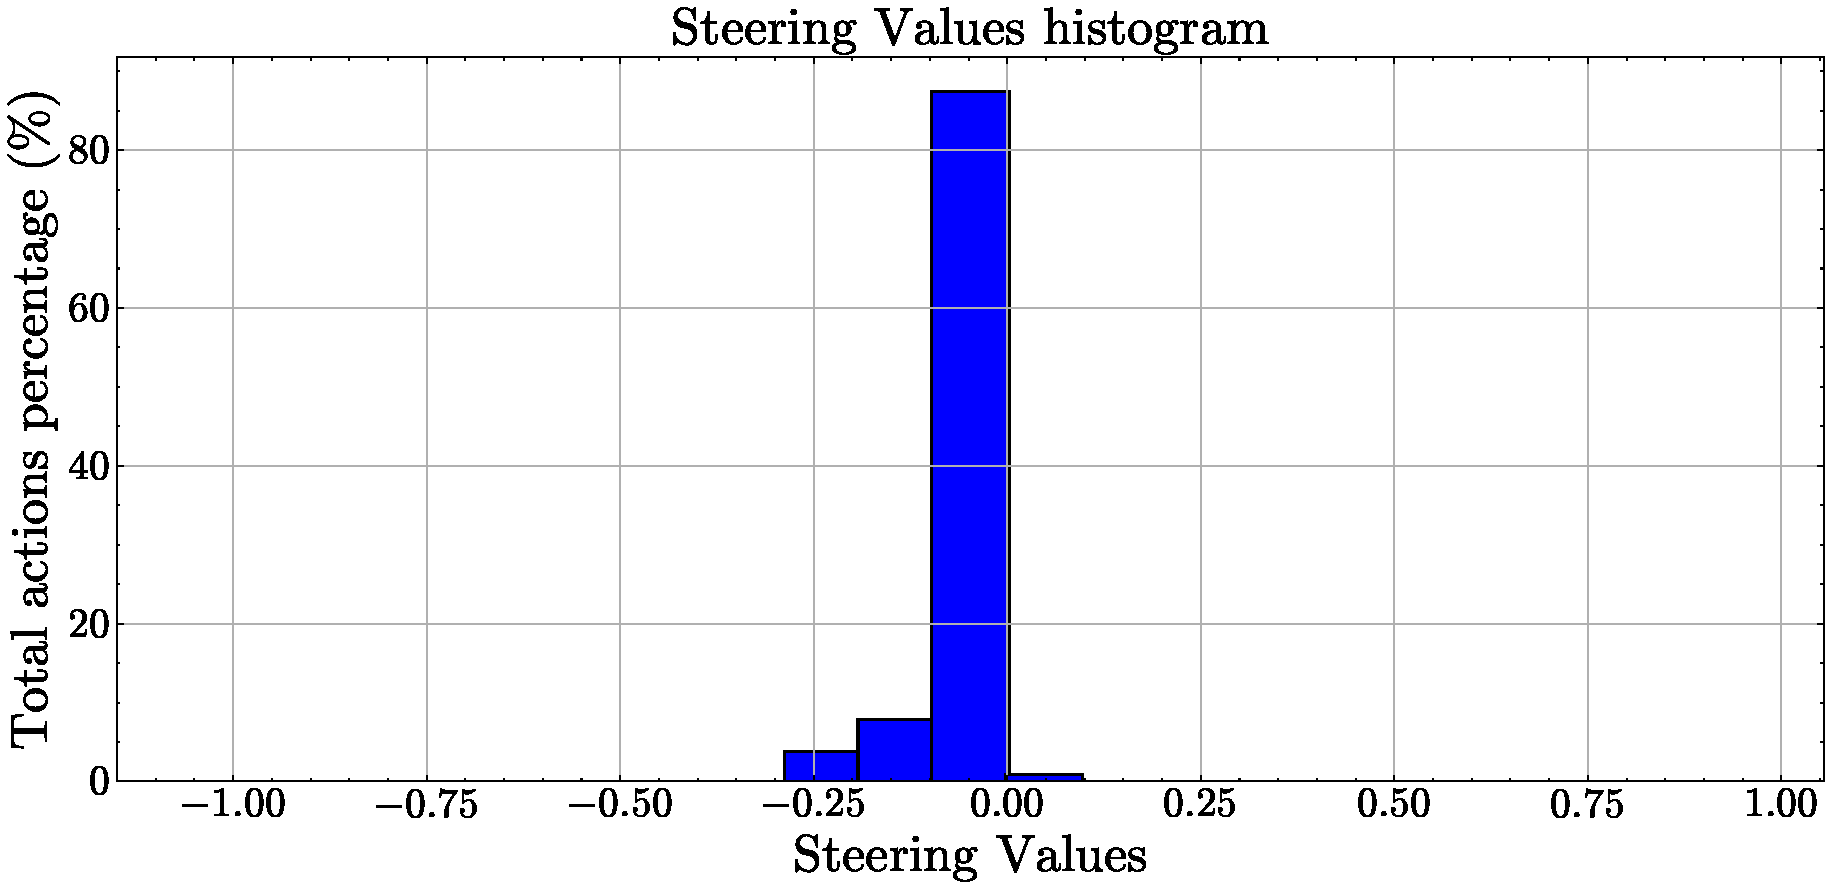
\includegraphics[height=5.9cm]{imagenes/cap4/sigue_carriles_qlearning/actions.pdf}
    \caption{Histograma de las acciones de giro tomadas por el sigue carril basado Q-learning}
    \label{fig:Histograma de las acciones de giro tomadas por el agente de Qlearning tras el entrenamiento}
\end{figure}


Tras terminar el proceso de entrenamiento, La última fase es evaluar los resultados del modelo obtenido. Aquí el algoritmo de Q-learning demostró un rendimiento altamente satisfactorio en la navegación por el carril. Q-learning mantuvo una conducción fluida y segura, sin giros bruscos y manteniendo una trayectoria recta, tal como se puede apreciar en la figura \ref{fig:Histograma de las acciones de giro tomadas por el agente de Qlearning tras el entrenamiento} donde podemos ver como el mayor porcentaje de movimientos son mantener el volante recto sin realizar ningún giro o realizar correcciones pequeñas sin efectuar giros abruptos.
  \begin{figure}[h]
    \centering
    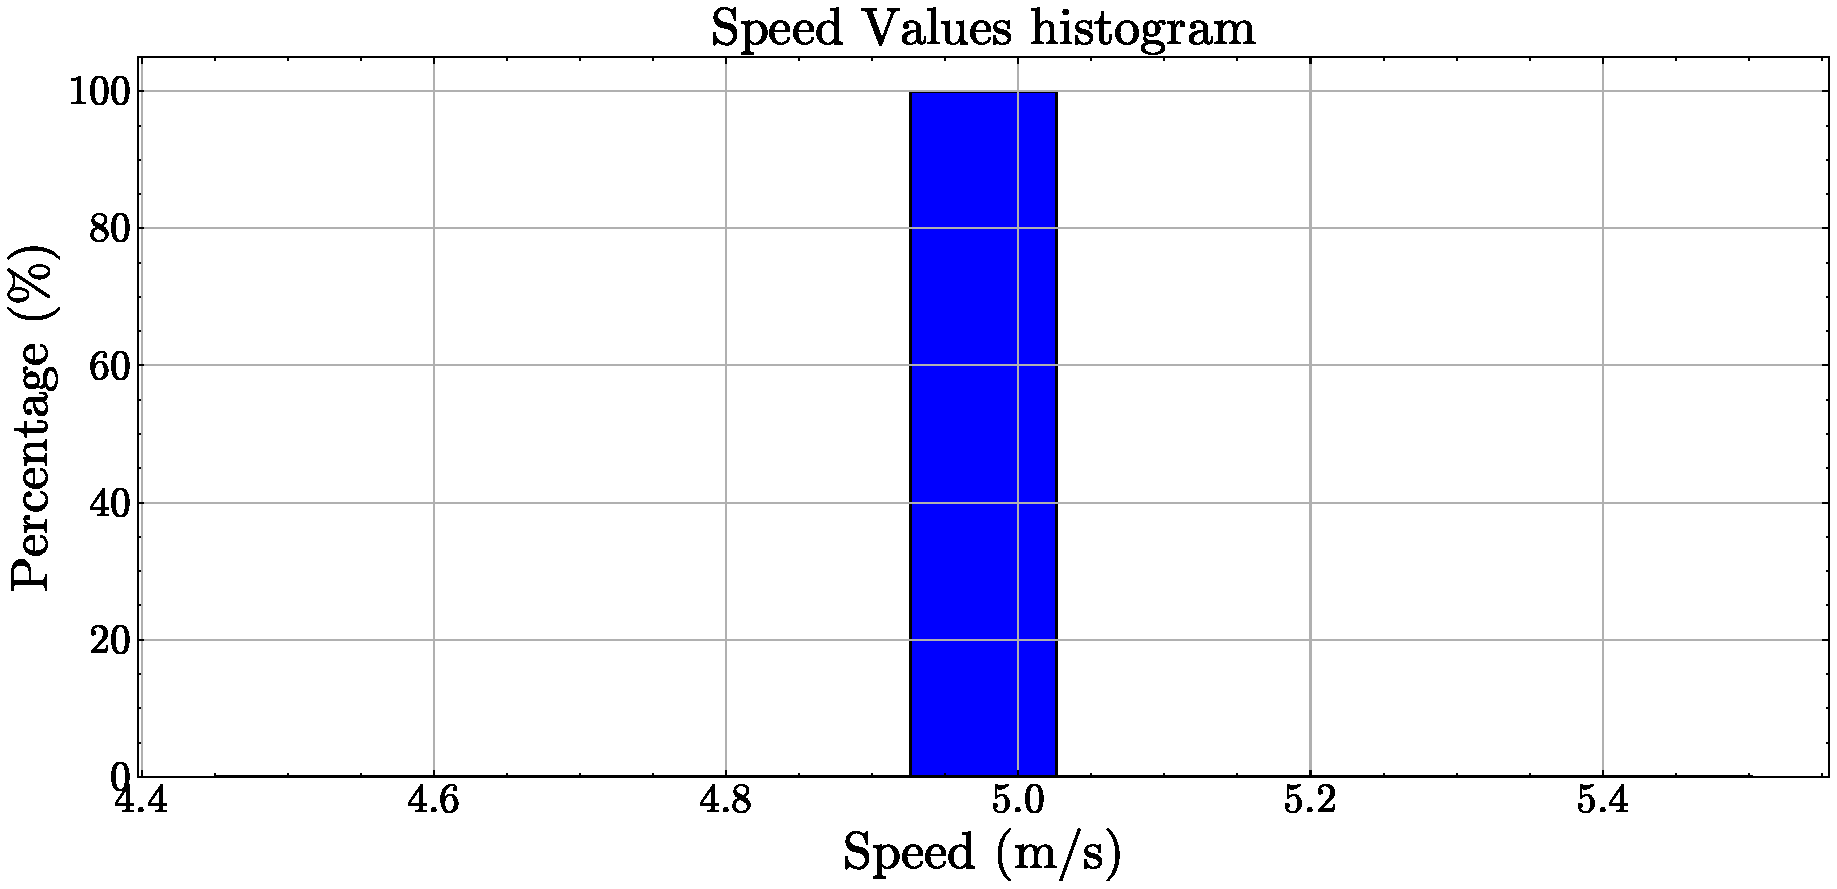
\includegraphics[height=6cm]{imagenes/cap4/sigue_carriles_qlearning/speeds.pdf}
    \caption{Histograma de las velocidades utilizadas por el sigue carril basado en Q-learning}
    \label{fig:Histograma de las velocidades utilizadas por el agente de Qlearning tras el entrenamiento}
\end{figure}

Además de esto en la gráfica de la figura \ref{fig:Histograma de las velocidades utilizadas por el agente de Qlearning tras el entrenamiento} también podemos ver como el vehículo siempre utiliza una velocidad lineal de 5 m/s la cuál es la velocidad más alta de la que dispone en sus acciones, esto debido a que como se ha comentado antes en la función recompensa se premian las velocidad altas siempre y cuando esto no genere salirse del carril


  \begin{figure}[h]
    \centering
    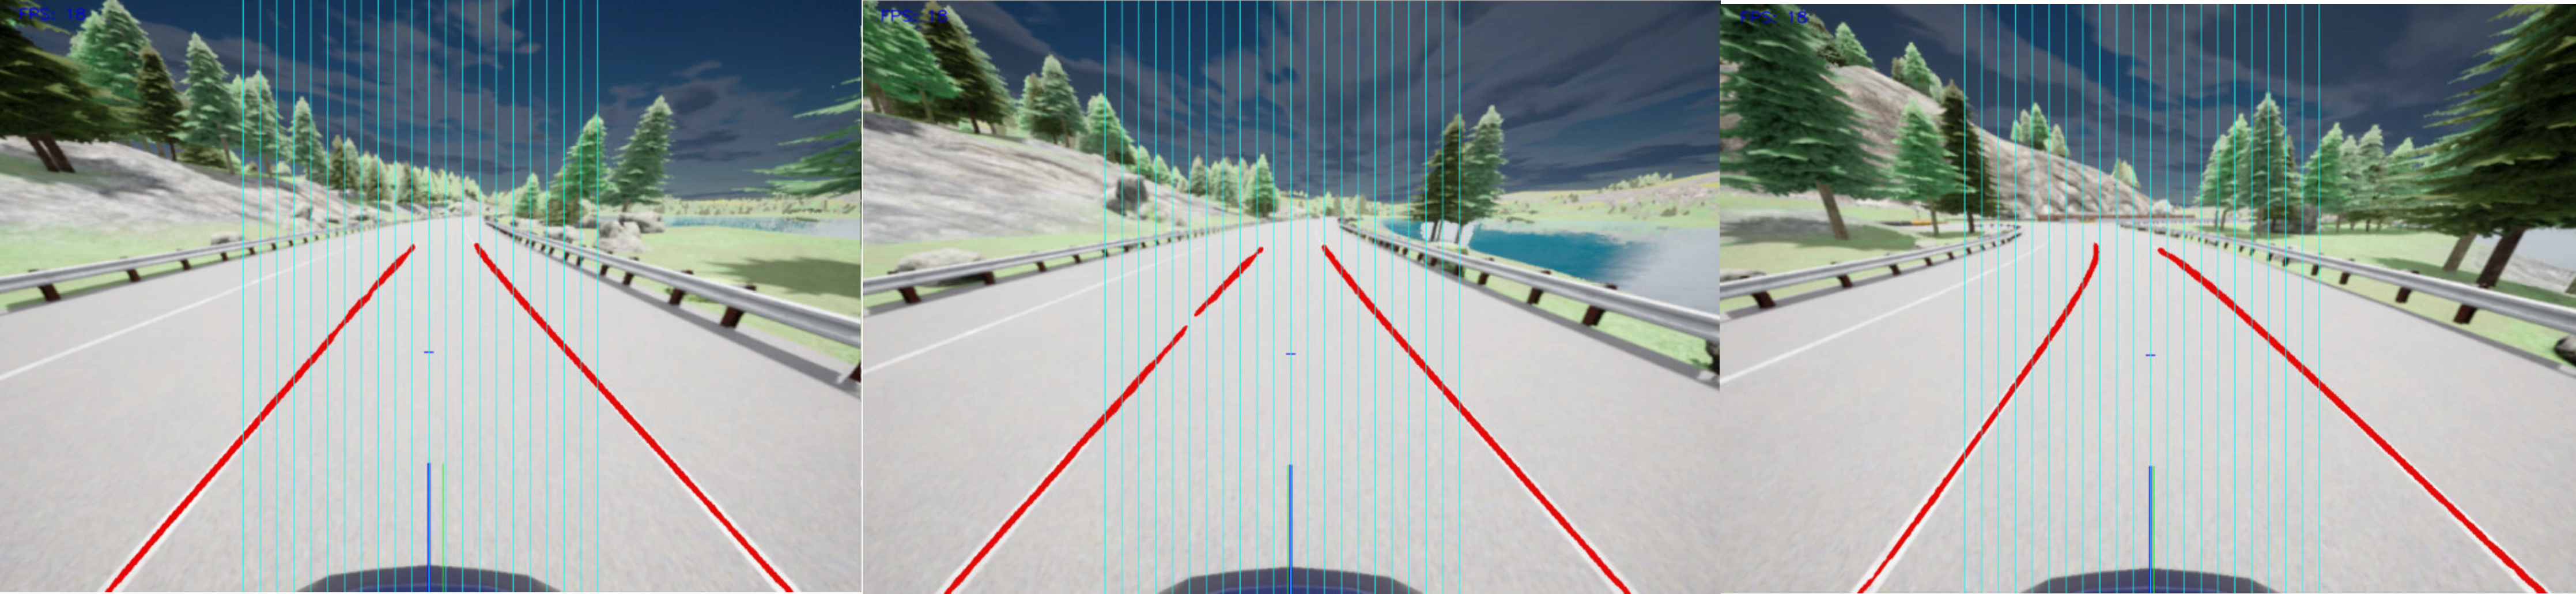
\includegraphics[height=3.5cm]{imagenes/cap4/demostraciones_qlearning/normal/demostracion_qlearning.pdf}
    \caption{Sigue carril basado en Q-learning}
    \label{fig:Sigue carriles basado en Qlearning}
\end{figure}


Como suele ser común al utilizar Q-learning el modelo entrenado final ofreció un resultado muy robusto y generalista, un ejemplo de la detección de este método en el entorno de entrenamiento puede verse en la figura \ref{fig:Sigue carriles basado en Qlearning}, pudiendo extrapolar el mismo modelo entrenado en el entorno de la figura \ref{fig:Entorno de entrenamiento del algoritmo de Q-learnig} a otras zonas aleatorias del mundo de CARLA las cuales no había visto nunca que se pueden ver en las figuras \ref{fig:Sigue carriles basado en Qlearning circuito 2} y \ref{fig:Sigue carriles basado en Qlearning circuito 3}, realizando en estos el seguimiento del carril presente en la vía sin problemas y de una manera fluida y segura, incluso en zonas con bajas luminosidad y curvas cerradas como se puede ver en la figura \ref{fig:Sigue carriles basado en Qlearning circuito 3}.

\bigskip

  \begin{figure}[h]
    \centering
    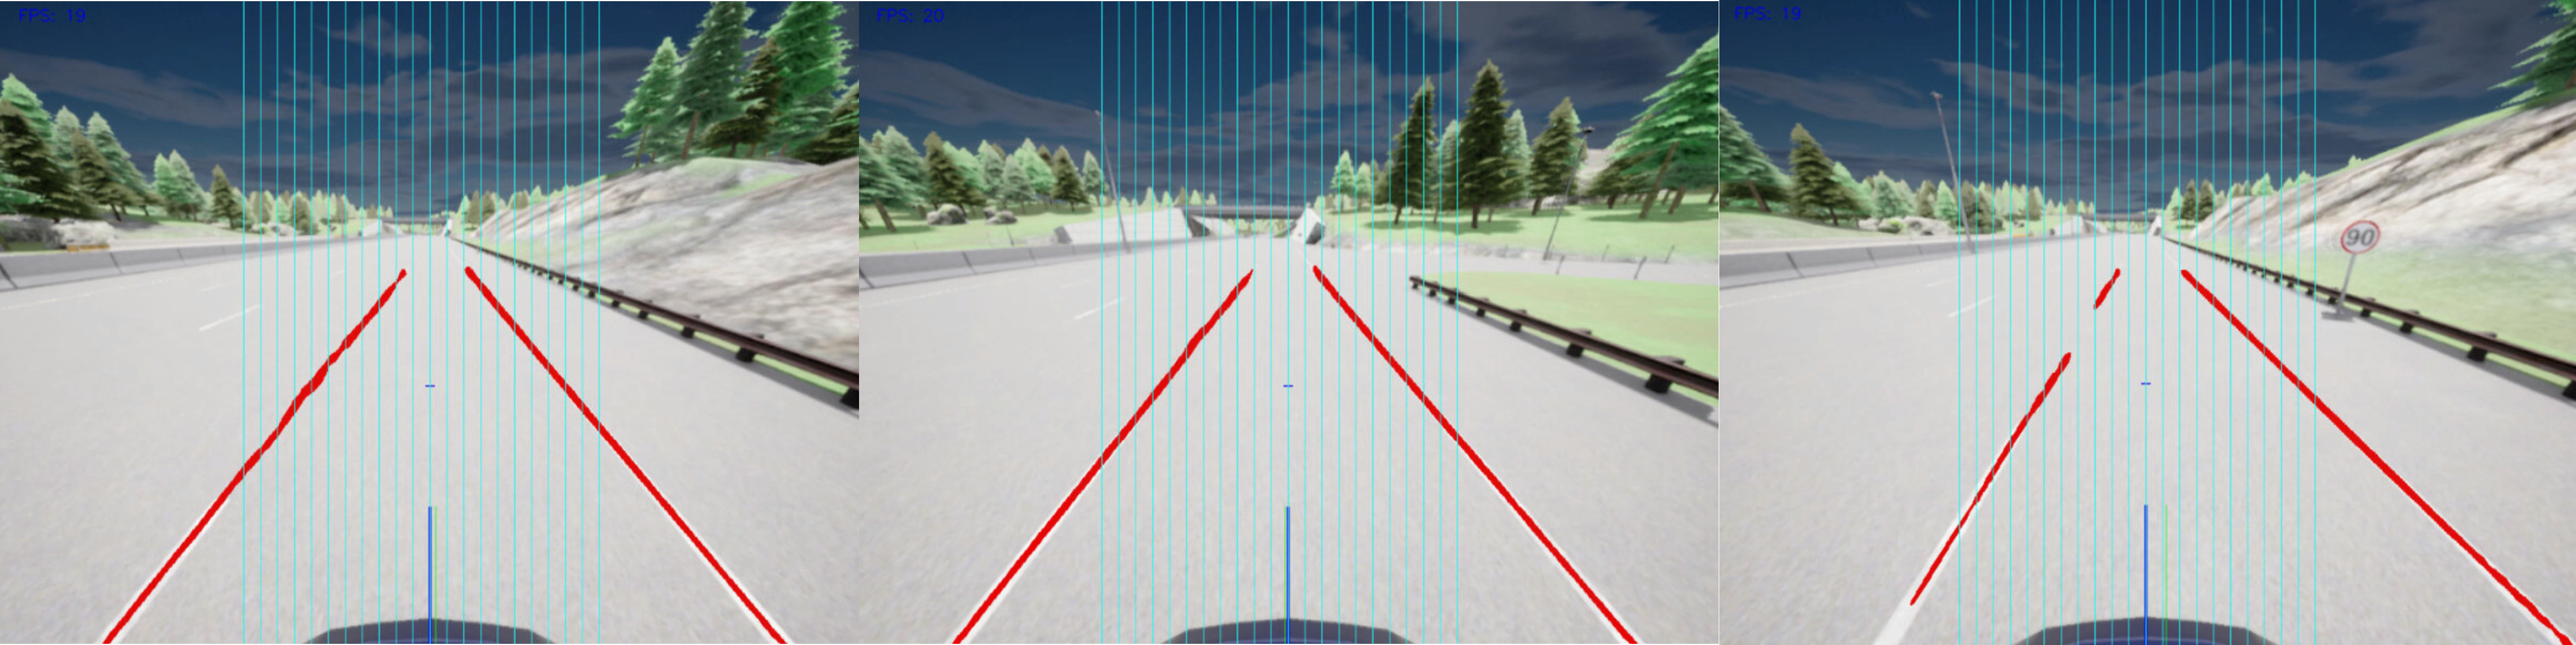
\includegraphics[height=4cm]{imagenes/cap4/demostraciones_qlearning/normal/qlearning_general/circuito_2/demostracion_escenario_1.pdf}
    \caption{Sigue carril basado en Q-learning zona 2 }
    \label{fig:Sigue carriles basado en Qlearning circuito 2}
\end{figure}

  \begin{figure}[h]
    \centering
    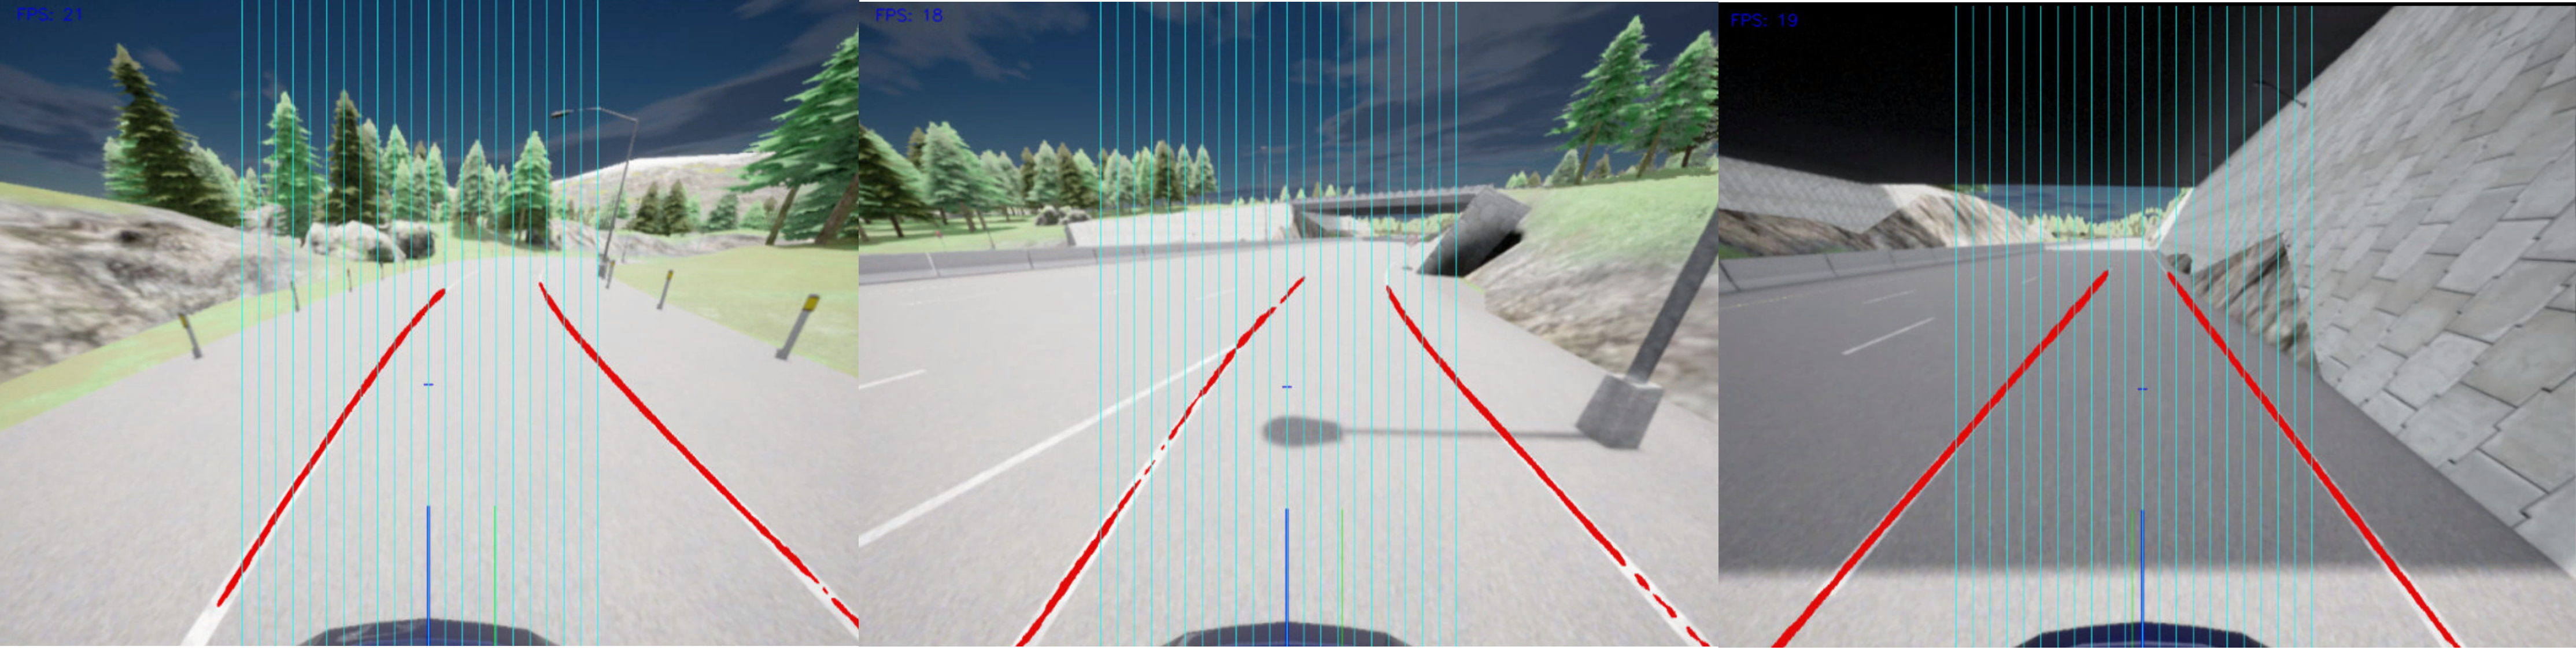
\includegraphics[height=4cm]{imagenes/cap4/demostraciones_qlearning/normal/qlearning_general/circuito_1/demostracion_escenario_2.pdf}
    \caption{Sigue carril basado en Q-learning zona 3}
    \label{fig:Sigue carriles basado en Qlearning circuito 3}
\end{figure}

\bigskip

Con esto concluimos que mientras la detección del carril sea precisa, se espera que el vehículo navegue de manera adecuada. por todo tipo de circuitos con curvas similares a las usadas en el entrenamiento. En esta \href{https://roboticslaburjc.github.io/2022-tfg-juancamilo-carmona/DEMOS/}{\textbf{entrada}} del blog del \ac{TFG} se pueden ver tres videos donde se observa el funcionamiento de este método de sigue carril en cada una de las zonas mostradas en las imagenes.


\subsection{Sigue carril con detención ante obstáculos en la vía}
\label{sigue carril con detención ante obstáculos en la vía}

En esta fase del proyecto, abordamos un nivel avanzado de complejidad en el sistema de seguimiento de carril. Además de lograr una conducción fluida en carreteras despejadas libres de objetos en la vía, nuestro objetivo ahora es garantizar que el vehículo pueda navegar de manera segura incluso cuando se enfrenta a obstáculos inesperados en la carretera, frenando el vehículo y deteniendo la marcha en casa de que esto ocurra y volviendo a reanudar la marcha una vez el obstáculo desaparezca. Para lograr esta funcionalidad, hemos integrado un sensor LIDAR en el vehículo, lo que nos permite detectar obstáculos en tiempo real y se ha modificado el algoritmo de Q-learning utilizado en la sección \ref{Sigue carril}.

\bigskip
Sin embargo, al implementar este método nos encontramos con un gran problema, y es que debido a la naturaleza del algoritmo Q-learning, cada estado va asociado a una acción y esta información es guardada en la tabla Q. Pero para lograr que esta implementación y que el agente se detuviera o navegara por el carril era necesario tener más de una acción asociada un estado debido a que podemos estar en un mismo estado con o sin un obstáculo delante y tener que tomar una acción distinta en cada caso. Para solventar este problema la solución que se planteo fue crear una segunda tabla Q, la cuál tuviera asociadas las acciones a ejecutar cuando apareciera un obstáculo. De esta manera la organización de este algoritmo sería la siguiente, tenemos dos tablas Q para diferentes situaciones:

  \begin{figure}[h]
    \centering
    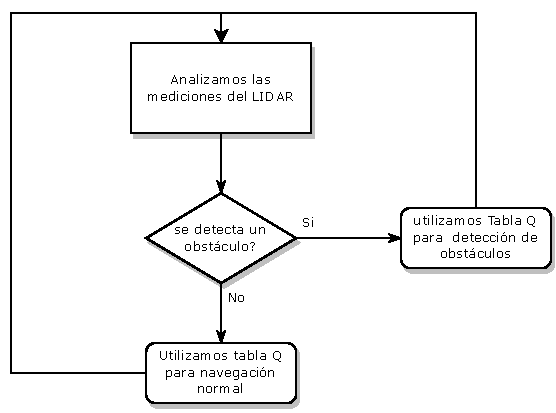
\includegraphics[height=7cm]{imagenes/cap4/evita_obstaculos_qlearning/diagrama_tabla_q.pdf}
    \caption{Diagrama de flujo de las tablas Q del sigue carril con detención ante obstáculos}
    \label{fig:Diagrama de flujo de las tablas Q del algoritmo con detencion ante obstáculos}
\end{figure}

\begin{enumerate}
    \item \textbf{Tabla Q para Navegación Normal:} En situaciones en las que no hay vehículos u obstáculos presentes en la carretera, el sistema utiliza una tabla Q diseñada para la navegación continua por el carril, como se ha demostrado en implementaciones anteriores. Esta tabla se enfoca en mantener una velocidad constante y un posicionamiento preciso en el carril.
    

    \item \textbf{Tabla Q para Detección de Obstáculos:} En situaciones en las que el sensor LIDAR detecta la presencia de un obstáculo, el sistema cambia automáticamente a una tabla Q especializada para abordar este escenario. La tabla Q de detección de obstáculos se centra en tomar decisiones que eviten colisiones con los obstáculos detectados. Esto incluye estrategias para detener el vehículo o realizar maniobras de evasión en función de la proximidad y tamaño del obstáculo.
\end{enumerate}

En el diagrama de flujo de la figura \ref{fig:Diagrama de flujo de las tablas Q del algoritmo con detencion ante obstáculos}  se puede ver de manera más visual este funcionamiento

\bigskip

Para lograr que esta idea de usar dos tablas Q funcione, es necesaria la realización de ciertos cambios clave en el código del algoritmo. Principalmente estos cambios debían realizarse en las funciones del programa que interactuaban con la tabla Q y consistían en añadir un if que determinara que tabla se iba a utilizar en función de la presencia o ausencia de un obstáculo detectado por el LIDAR. En el código \ref{cod:Función para elegir una acción de la tabla Q del algoritmo con reacción a obstáculos} se puede ver un ejemplo del if que controla el cambio de tabla Q en la función de elección de acciones de la implementación de Q-learning

\begin{code}[H]
	\begin{lstlisting}[language=Python]
    def choose_action(self, state):
	
       #this if determines which Q table we will use
        if self.object_in_front:
            current_q_table = self.q_table_with_object
        else:
            current_q_table = self.q_table_without_object
    
        if np.random.uniform(0, 1) < self.exploration_rate:
            action = np.random.randint(len(self.ACTIONS))
            self.random_counter += 1
        else:
            action_values = current_q_table[state]
            action = np.unravel_index(action_values.argmax(), action_values.shape)[0]
            self.table_counter += 1

        return action
	\end{lstlisting}
\caption[Función para elegir una acción leyendo la tabla Q del sigue carril con detención ante obstáculos]{Función para elegir una acción leyendo la tabla Q del sigue carril con detención ante obstáculos}
\label{cod:Función para elegir una acción de la tabla Q del algoritmo con reacción a obstáculos}
\end{code}

\bigskip

En adición a esto una modificación de la función recompensa también es necesaria para conseguir que el agente recibiera las recompensas correctas para lograr el nuevo comportamiento, estos consistieron en lo siguiente:

\begin{itemize}
    \item En ausencia de obstáculos, la función de recompensa premia la navegación continua y efectiva por el carril, como se ha hecho en las implementaciones anteriores. Se premia mantener una velocidad alta, una posición central en el carril y un angulo paralelo con las líneas del mismo.
    
    \item Cuando se detecta un obstáculo, la función de recompensa otorga la máxima recompensa si el vehículo se detiene por completo para evitar una colisión inminente con el obstáculo. De forma análoga se otorga la mínima recompensa al agente si al detectar un obstáculo este no se detiene.
\end{itemize}

\bigskip

En el código \ref{cod:Función recompensa del algoritmo con reacción a obstáculos} podemos ver la función recompensa actualizada con los cambios descritos

\begin{code}[H]
	\begin{lstlisting}[language=Python]
    def reward_function(self, error, angle_error,car_crashed):

	#if we dont stop after detecting an object min. reward is given
        if not self.object_in_front and self.speed == 0.0:
            reward = 0.0
            return reward
	
	#if we stop after detecting an obstacle max. reward is given
        elif self.object_in_front and self.speed == 0.0:
            reward = 1.0
            return reward

        if self.lane_lines < 1:
            reward = 0.0
            return reward
        
        if car_crashed:
            reward = 0.0
            return reward


        normalized_error = abs(error)

        reward = ((((1 / (normalized_error + 1)) + self.speed/100) - angle_error/100))

        reward = np.clip(reward, -1.0, 1.0)

        reward = 1 / (1 + np.exp(-reward))

        print("reward: ", reward)
        return reward
	\end{lstlisting}

\caption[Función recompensa del sigue carril con detención ante obstáculos]{Función recompensa del sigue carril con detención ante obstáculos}
\label{cod:Función recompensa del algoritmo con reacción a obstáculos}
\end{code}
\bigskip

En cuanto a las acciones, estas no variaron con respecto a las vistas en la figura \ref{cod:Acciones disponibles para el algoritmo de qlearning}, la única modificación fue la sustitución de la velocidad más bajas disponible, que en este caso era 3.5 m/s por una velocidad nula.Con este cambio conseguimos una velocidad que nos permite frenar el vehículo y detener su marcha en caso de encontrarnos obstáculo. Aplicando este cambio las acciones de velocidad de este algoritmo se corresponden con las que se pueden ver en la figura \ref{cod:Acciones disponibles para el algoritmo de qlearning con reaccion ante obstaculos}. Los estados por otro lado permanecen iguales que los utilizados en el método anterior vistos en la figura \ref{fig:Estados del algoritmo de Q-learnig}


    \bigskip
    \begin{code}[H]
	\begin{lstlisting}[language=Python]
        ]
        self.SPEED = [ 
            'speed_1',   #stering = 0 m/s  
            'speed_2',   #stering = 4.0 m/s  
            'speed_3',   #stering = 4.5 m/s
            'speed_4'    #stering = 5.0 m/2        ]
	\end{lstlisting}
\caption[Acciones de velocidad del sigue carril con detención ante obstáculos]{Acciones de velocidad del sigue carril con detención ante obstáculos}
\label{cod:Acciones disponibles para el algoritmo de qlearning con reaccion ante obstaculos}
\end{code}

\bigskip

Otra ventaja clave de este concepto de utilizar dos tablas Q es su alta modularidad y flexibilidad. La incorporación de dos tablas Q distintas, brinda la capacidad de entrenar y operar cada contexto por separado. En primer lugar, podemos entrenar la tabla Q destinada a la navegación en carriles despejados, perfeccionando así las habilidades de conducción fluida y segura en condiciones ideales. Simultáneamente, podemos llevar a cabo el entrenamiento de la tabla Q específica para la detección de obstáculos. Esto implica enseñar al vehículo a reaccionar adecuadamente cuando se encuentre con un obstáculo en la carretera. Una vez que ambas tablas Q estén entrenadas y afinadas de manera óptima, el sistema puede operar en dos modos distintos: en modo carretera despejada y en modo detección de obstáculos. Incluso se podría solo entrenar la tabla Q de detención ante obstáculos y en el caso la tabla de navegación utilizar una tabla ya entrenada y que este dando buenos resultados, como por ejemplo la del primer método se seguimiento de carril basado en Q-learning \ref{Sigue carril} 

\bigskip

Una vez finalizada la implementación del algoritmo, avanzamos a la fase de entrenamiento, siguiendo la misma metodología que en la sección anterior. Para este proceso, se dejó entrenar el modelo en el servidor Landau de la universidad, pero con una duración extendida en comparación a la implementación \ref{fig:Sigue carriles basado en Qlearning} de aproximadamente 24 horas esto debido a que entrenar dos tablas Q de manera correcta y el tiempo de detención ante obstáculos suponía una tarea más demorada que la de entrenar una sola tabla de un algoritmo que nunca de paraba. De esta manera la gráficas que obtenemos luego de este entrenamiento resultan muy parecidas a las anteriores. donde la gráfica de la recompensa acumulada que se puede ver en la figura \ref{fig:Evolución de la recompensa acumulada del algoritmo sigue carril con reacción a obtáculos} es muy similar a la del método \ref{Sigue carril}  pero convergiendo ahora recompensas más altas, debido a las altas premiaciones que obtiene nuestro algoritmo al detenerse ante obstáculos.


  \begin{figure}[h]
    \centering
    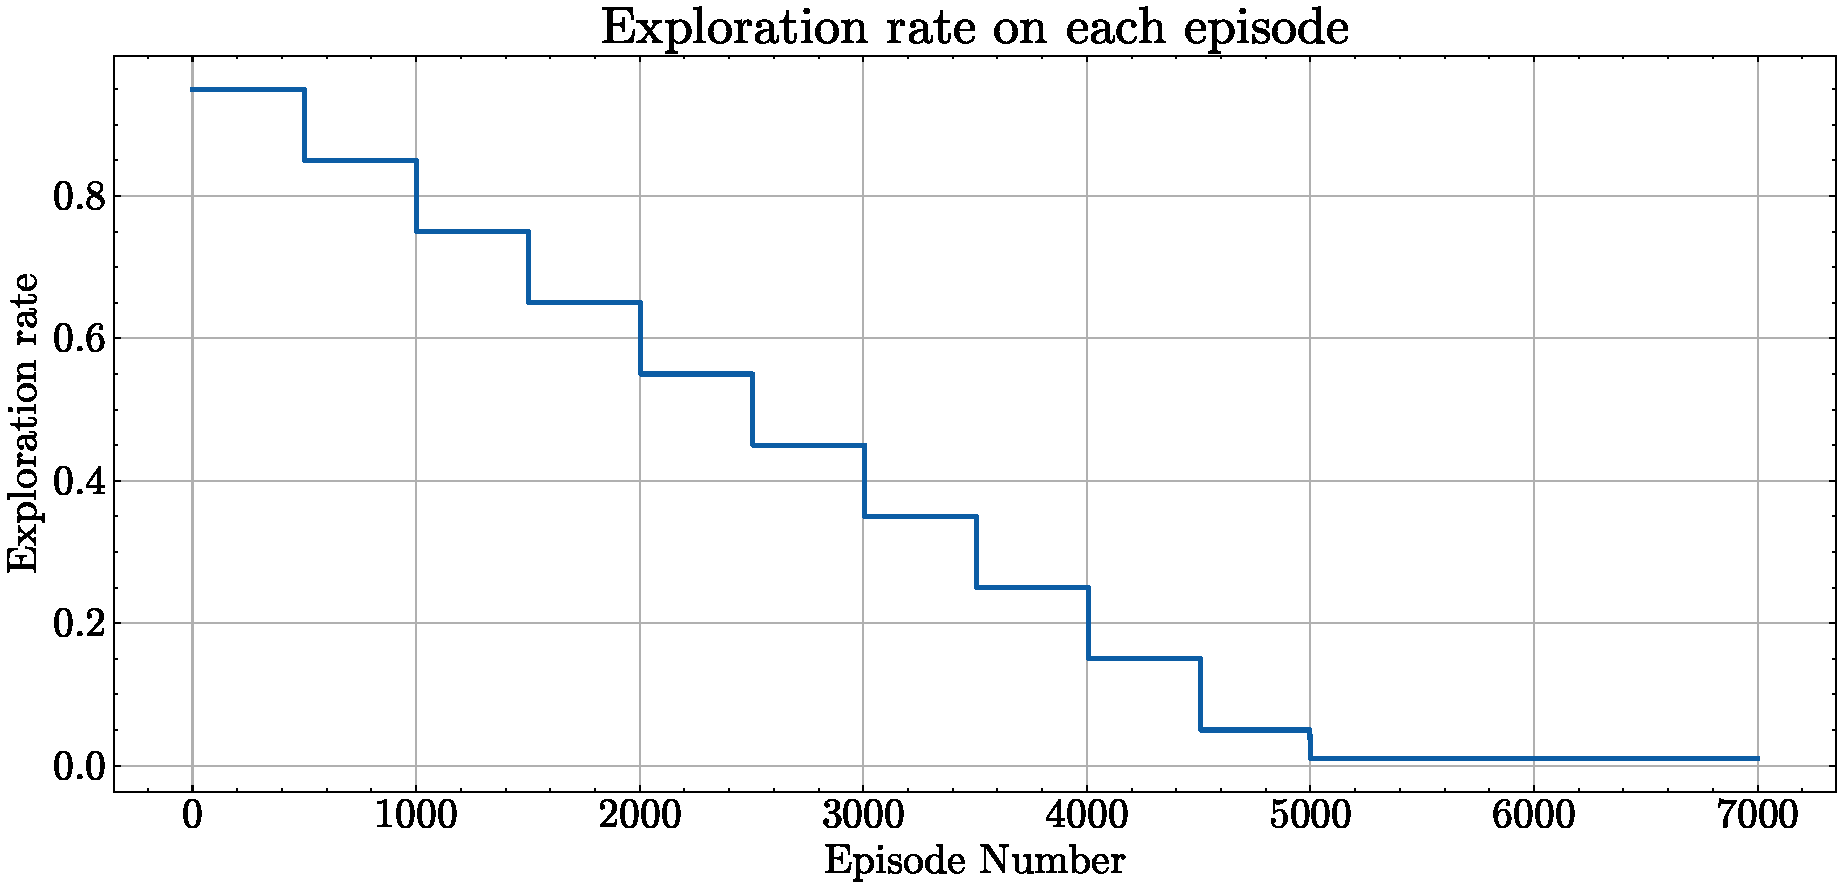
\includegraphics[height=6cm]{imagenes/cap4/sigue_carriles_qlearning/exploration_rate.pdf}
    \caption{Evolución del ratio de exploración del sigue carril con detención ante obtáculos}
    \label{fig:Evolución del ratio de exploración del algoritmo sigue carril con reacción a obtáculos}
\end{figure}

  \begin{figure}[h]
    \centering
    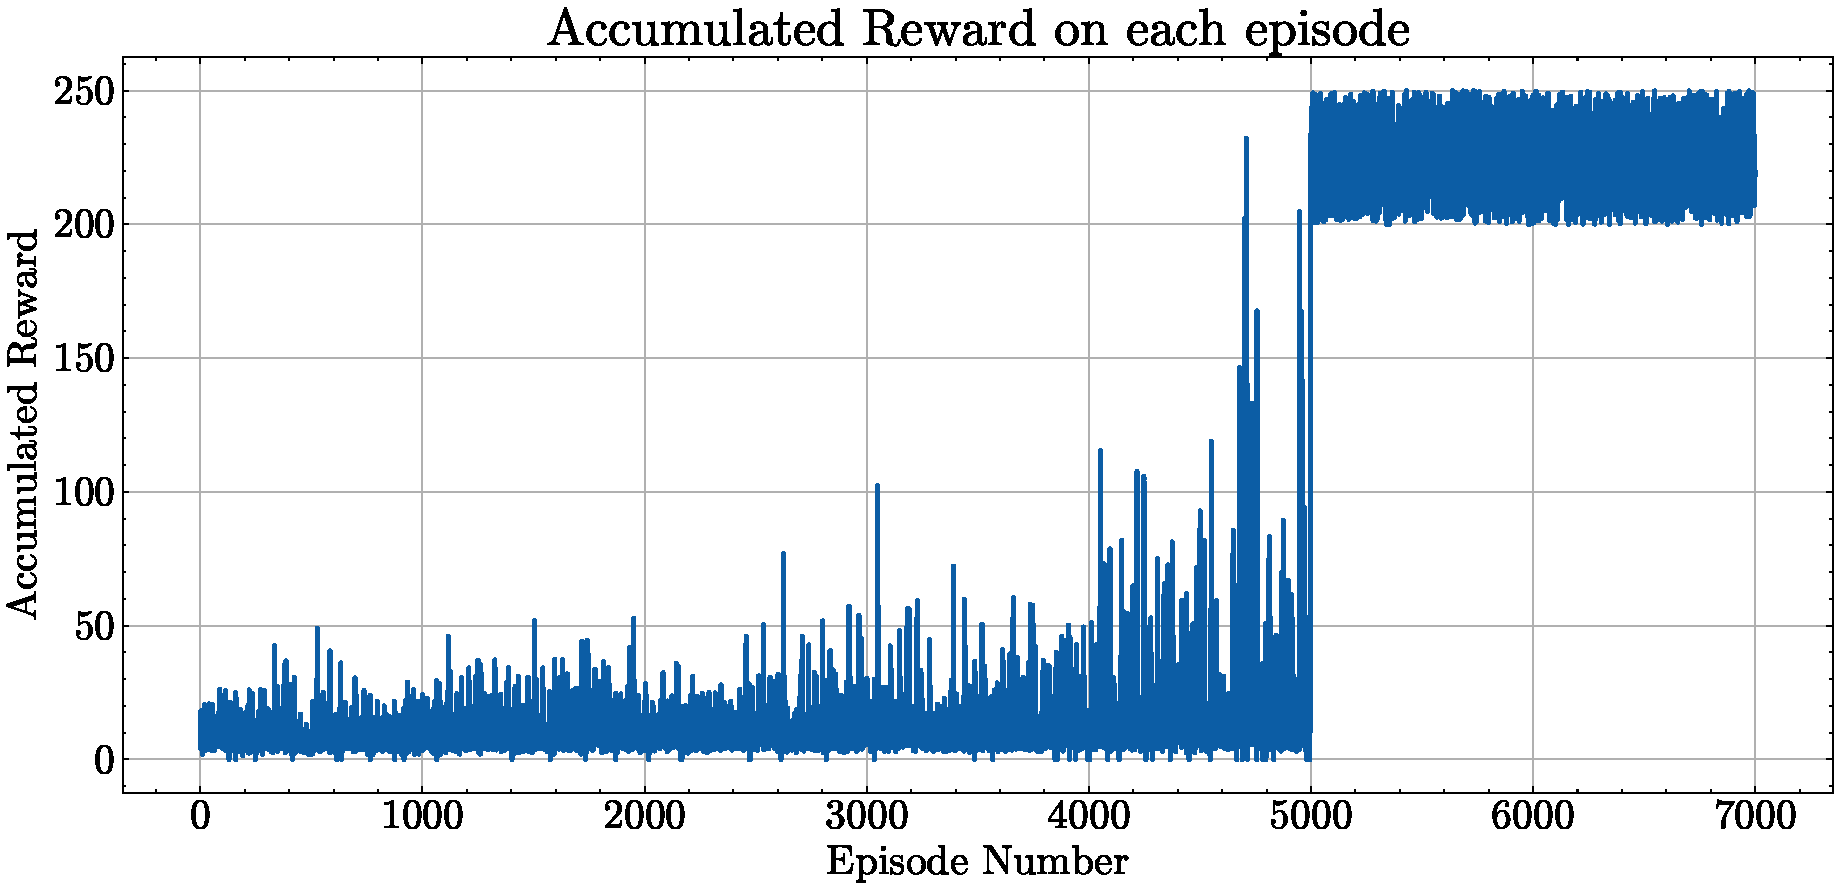
\includegraphics[height=6cm]{imagenes/cap4/evita_obstaculos_qlearning/recompense.pdf}
    \caption{Evolución de la recompensa acumulada del sigue carril con detención obtáculos}
    \label{fig:Evolución de la recompensa acumulada del algoritmo sigue carril con reacción a obtáculos}
\end{figure}


En cuanto a la gráfica de acciones observables en la figura \ref{fig:Histograma de acciones del algoritmo sigue carril con reacción ante obstáculos} nuemavemente podemos comprobar que la mayoría de acciones de giro ejecutadas por nuestro agente son la ausencia de giro, dejado el volante si mover o giros pequeños que no resultaran muy bruscos y favorecieran una conducción fluida muy similar a la gráfica del método anterior vista en la figura \ref{fig:Histograma de las acciones de giro tomadas por el agente de Qlearning tras el entrenamiento}.

  \begin{figure}[t]
    \centering
    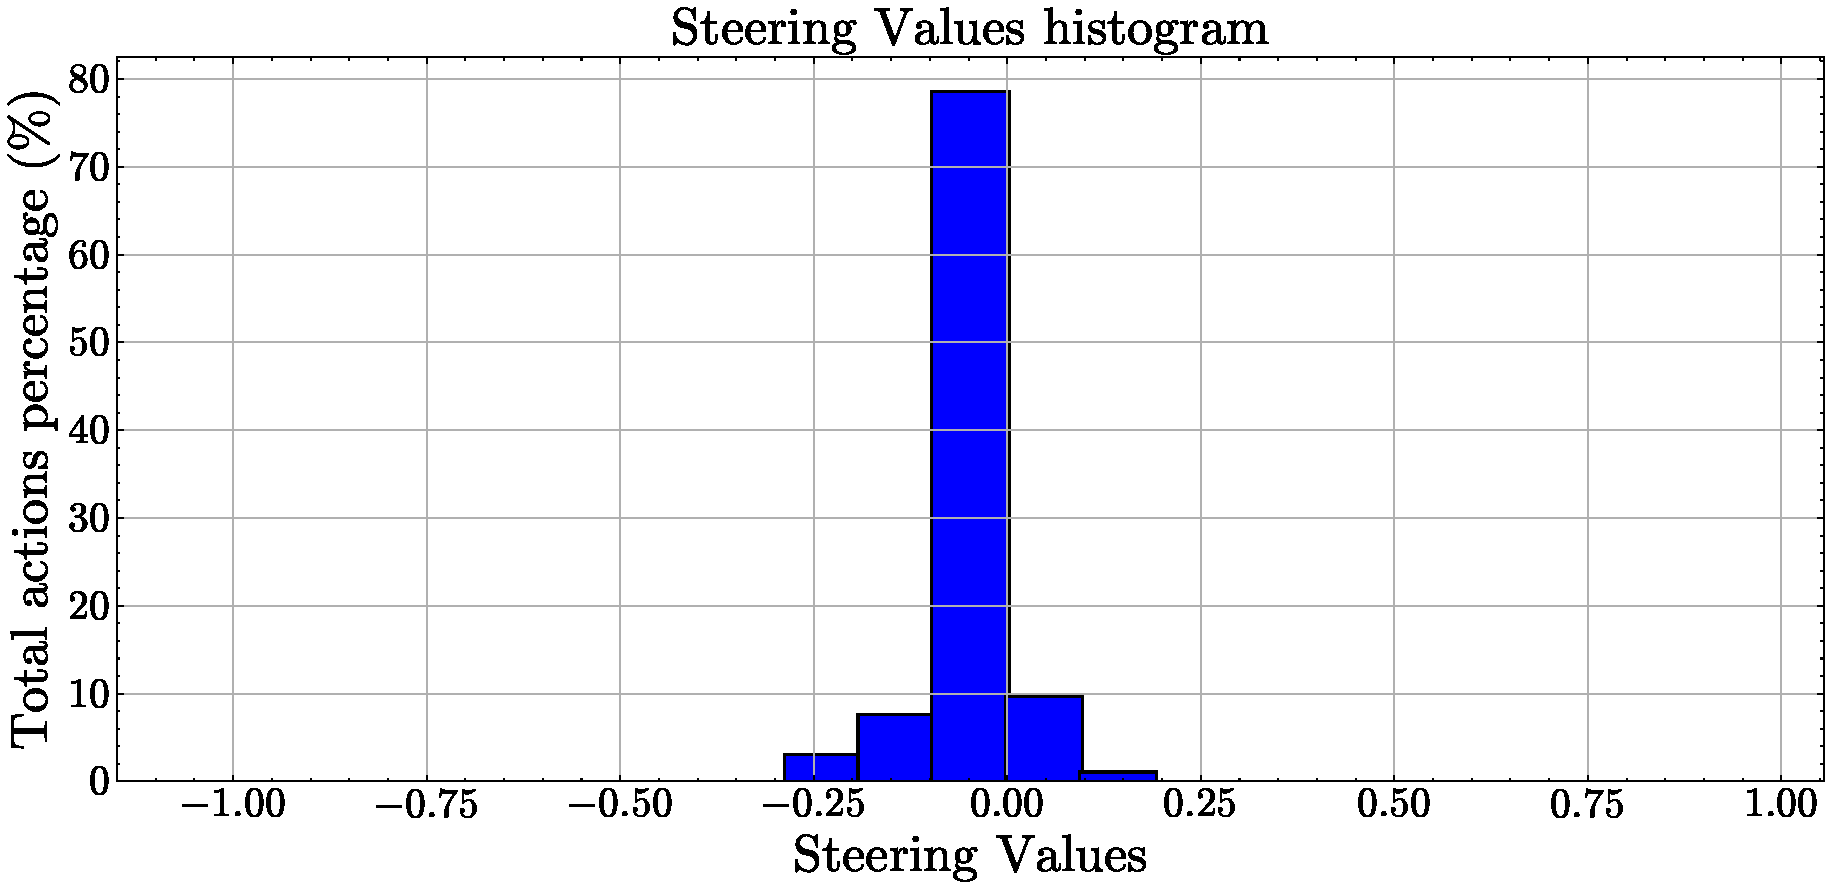
\includegraphics[height=6cm]{imagenes/cap4/evita_obstaculos_qlearning/actions.pdf}
    \caption{Histograma de acciones de giro del sigue carril con detención ante obstáculos}
    \label{fig:Histograma de acciones del algoritmo sigue carril con reacción ante obstáculos}
\end{figure}
        

\bigskip

Sin embargo, en la gráfica de las velocidades utilizadas por nuestro vehículo encontramos una peculiaridad con respecto a la de la figura \ref{fig:Histograma de las velocidades utilizadas por el agente de Qlearning tras el entrenamiento} correspondiente al método anterior. Y es que si nos fijamos en el histograma de la figura \ref{fig:Histograma de las velocidades del algoritmo sigue carril con reacción ante obstáculos} podemos ver como ahora nuestro vehículo utiliza distintas velocidades. Ahora un porcentaje de las velocidades que utiliza el vehículo son 0 m/s esto se debe naturalmente a que cuando aparece un obstáculo en la vía nuestro vehículo se detiene hasta que este sea retirado por lo que no tiene ninguna velocidad lineal, aparte de esto vemos como también que hay un pequeño porcentaje de velocidades cercanas a 5 m/s estas son causadas por elecciones del algoritmo a la hora de reanudar la marcha ya para no pegar giros muy bruscos.
\bigskip

  \begin{figure}[h]
    \centering
    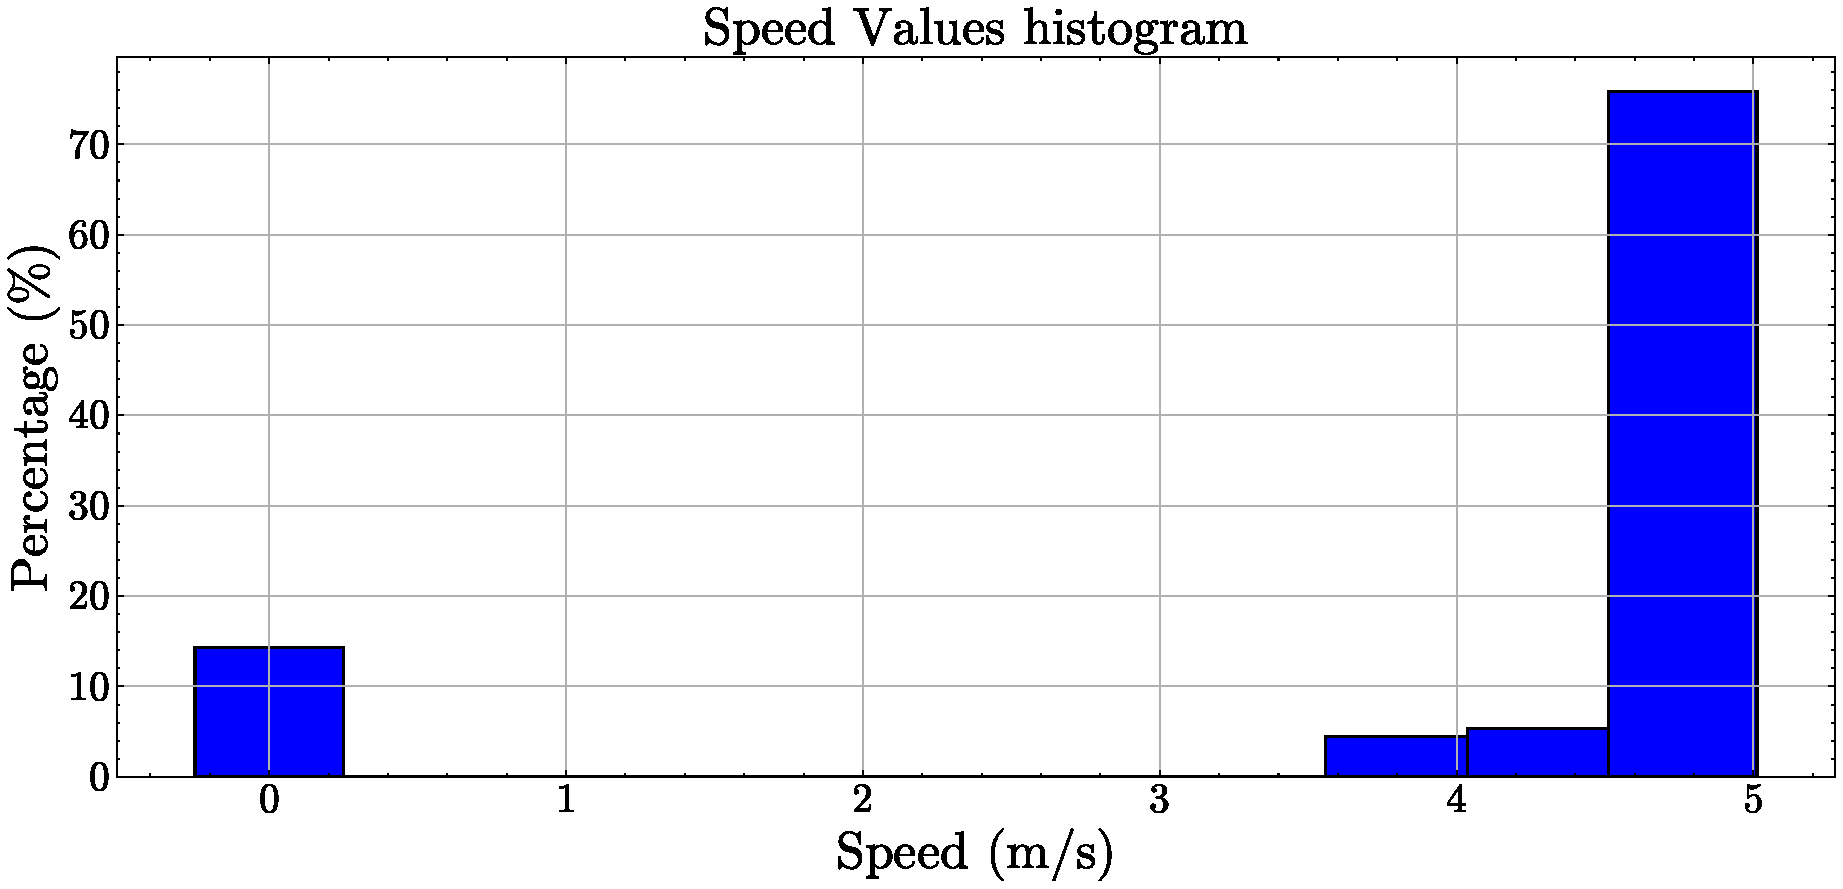
\includegraphics[height=6cm]{imagenes/cap4/evita_obstaculos_qlearning/speeds.pdf}
    \caption{Histograma de las velocidades del sigue carril con detención ante obstáculos}
    \label{fig:Histograma de las velocidades del algoritmo sigue carril con reacción ante obstáculos}
\end{figure}

Como conclusión los resultados del entrenamiento son altamente satisfactorios para este método, generando un modelo capaz de conducir de manera fluida por un carril y que en caso de encontrarse un obstáculo, como se ve en la figura \ref{fig:Sigue carriles con deteción ante obstáculos basado en Qlearning}, detener la marcha, hasta que este sea retirado de la carretera. Una demostración más visual de este comportamiento se puede observar un video en esta \href{https://roboticslaburjc.github.io/2022-tfg-juancamilo-carmona/DEMOS/}{\textbf{entrada}} del blog del \ac{TFG}.
\bigskip

  \begin{figure}[h]
    \centering
    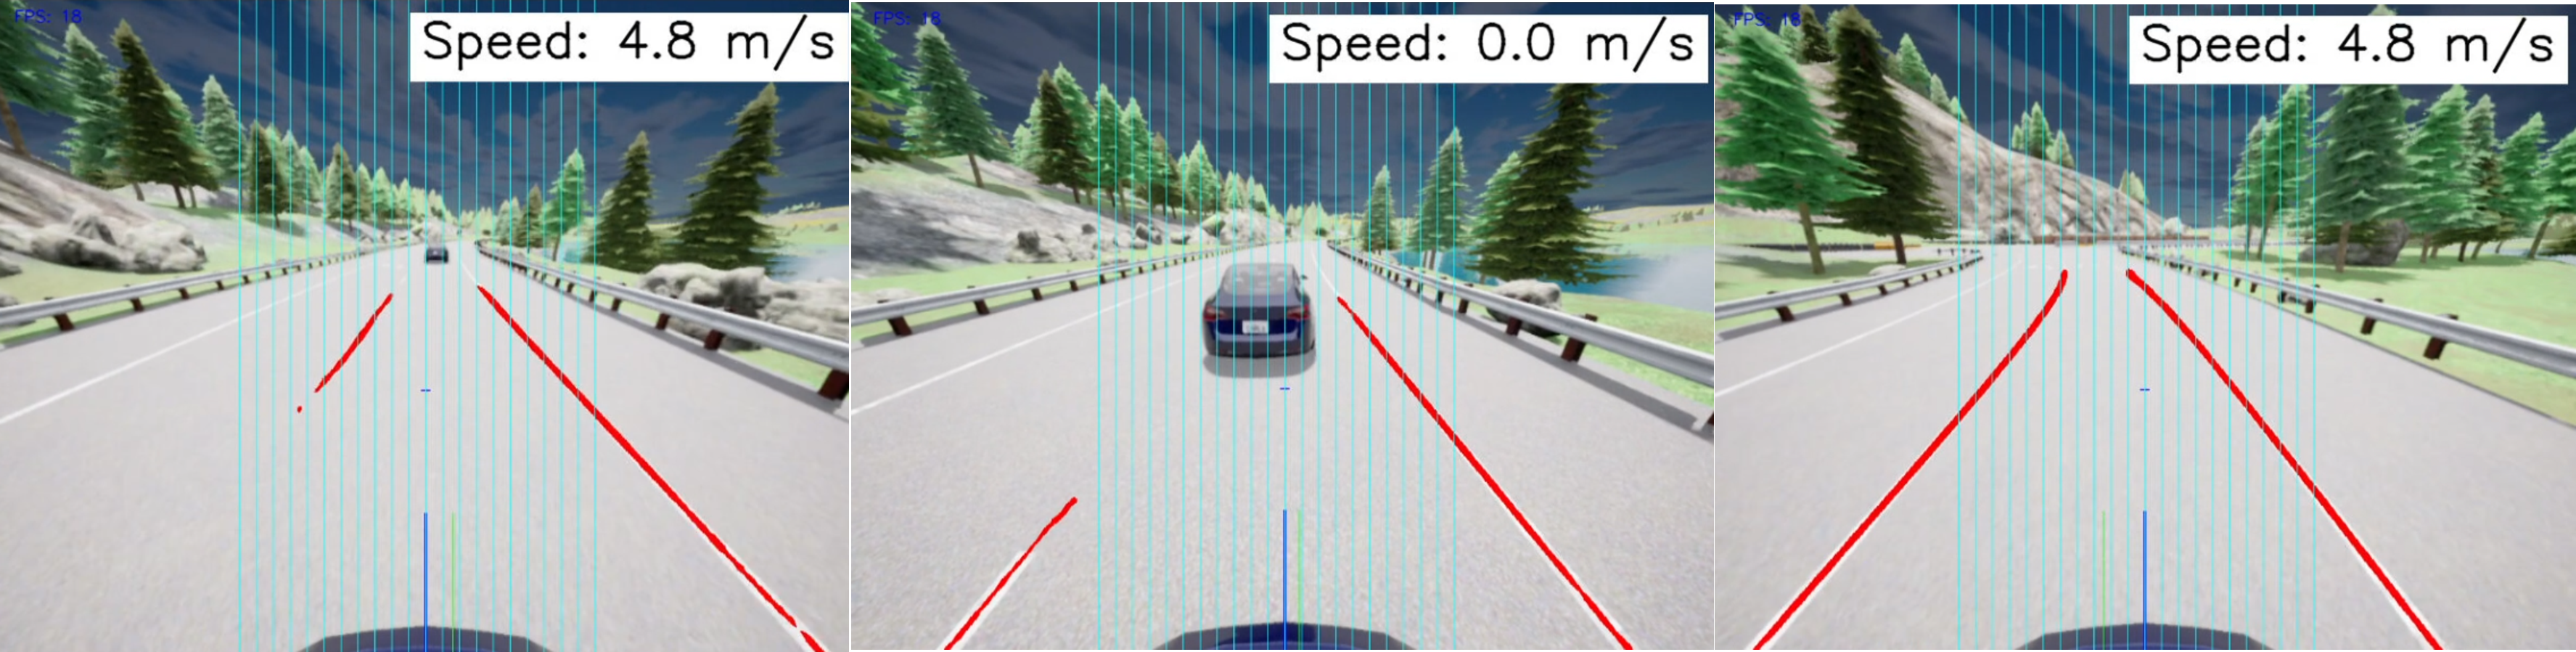
\includegraphics[height=3.5cm]{imagenes/cap4/demostraciones_qlearning/obstacle/demostracion_sigue_carriles.pdf}
    \caption{Sigue carril con detención ante obstáculos}
    \label{fig:Sigue carriles con deteción ante obstáculos basado en Qlearning}
\end{figure}

\subsection{Sigue carril con adaptación al tráfico}
\label{Sigue carril con adaptación al tráfico}

La última y más compleja implementación en este \ac{TFG} es un sistema de seguimiento de carriles capaz de adaptarse al tráfico presente en el carril. En este escenario, el vehículo debe tomar decisiones inteligentes tanto cuando se encuentra en condiciones de carretera despejada como cuando se enfrenta a obstáculos o vehículos en movimiento que circulan con una velocidad más lenta que la suya. Para lograr esta adaptación al tráfico, nuevamente se utiliza un sensor LIDAR, pero en este caso para medir la distancia al obstáculo o vehículo de adelante.

Para esta implementación se volverá usar la técnica de utilizar mas de una tabla Q, pero en este caso se utilizan 4 tablas, ya que se han establecido varios umbrales de distancia, dividiendo el rango de medición en segmentos que van desde 0 a 3 metros, de 3 a 8 metros y de 8 a 12 metros. Dependiendo de en qué rango se encuentre el vehículo de adelante, se utiliza una tabla Q u otra de manera que cada tabla Q tendrá asociadas distintas velocidades y las acciones de giro necesarias para esas velocidades, para esto modificaremos la función de recompensa de manera que:

\begin{itemize}
	\item Una tablas Q sirva para navegar sin obstáculos
	\item Otra de las tablas sirva para obstáculos cercanos en un rango de 0 a 3 metros en la que premiaremos detener el vehículo
	\item Otra de las tablas sirva para obstáculos a una distancia media entre 3 y 8 metros de distancia, en esta tabla Q premiaremos utilizar una velocidad media
	\item La última tabla Q sirva para obstáculos lejanos en un umbral de 8 a 12 metros, en esta tabla Q recompensaremos una velocidad medio alta.
   
\end{itemize}

\bigskip

Una representación más visual de este funcionamiento se puede ver en el diagrama de flujo de la figura \ref{fig:Diagrama de flujo de las tablas Q del algoritmo con adaptación al tráfico}

  \begin{figure}[h]
    \centering
    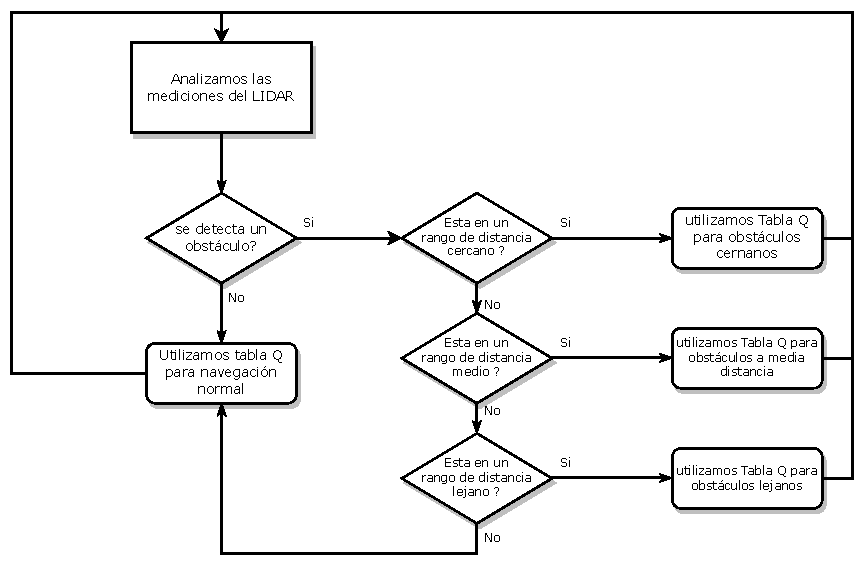
\includegraphics[height=8cm]{imagenes/cap4/adaptacion_trafico_qlearning/diagrama_tabla_q_trafico.pdf}
    \caption{Diagrama de flujo de las tablas Q del sigue carril con adaptación al tráfico}
    \label{fig:Diagrama de flujo de las tablas Q del algoritmo con adaptación al tráfico}
\end{figure}

Las acciones también se modificaran para ofrecerle a nuestro agente una variedad de acciones que le permitan adaptarse a un tráfico más lento, de esta manera ahora las acciones de velocidad disponibles para el agente de Q-learning serán 0 m/s, 2 m/s y 3 m/s tal como se observa en el código \ref{cod:Acciones disponibles para el algoritmo de qlearning con adaptación al tráfico}. Las acciones de giro de dirección y los estados por otro lado se mantienen iguales a los de los dos métodos anteriores. Los estados se pueden ver en la figura  \ref{fig:Estados del algoritmo de Q-learnig} y las acciones de giro en el código \ref{cod:Acciones disponibles para el algoritmo de qlearning}

    \begin{code}[H]
	\begin{lstlisting}[language=Python]
        ]
        self.SPEED = [ 
            'speed_1',   #stering = 0 m/s  
            'speed_2',   #stering = 2.0 m/s  
            'speed_3',   #stering = 3.0 m/s
            'speed_4'    #stering = 5.0 m/2        ]
	\end{lstlisting}
\caption[Acciones de velocidad del sigue carril con adaptación al tráfico]{Acciones de velocidad del sigue carril con adaptación al tráfico}
\label{cod:Acciones disponibles para el algoritmo de qlearning con adaptación al tráfico}
\end{code}

Para conseguir esto crearemos una nueva implementación de la función recompensa que se puede ver en el código \ref{cod:Función recompensa del algoritmo con adaptación al tráfico}. La función de recompensa se modifica para premiar la toma de decisiones que mantienen una distancia segura con el vehículo de adelante y permita una adaptación eficiente al tráfico. Se otorga una recompensa máxima al agente cuando utiliza la velocidad adecuada para el rango de distancia en el que se encuentre con respecto al vehículo de adelante. También se modificarán las velocidades disponibles para nuestro agente dejando la velocidad 5 m/s para navegas en ausencia de obstáculos y luego y añadiendo las velocidades  0 m/s , 2.0 m/s  y 3.5 m/s para ser utilizadas cada una en un umbral de distancia distinto.

\bigskip

\begin{code}[H]
	\begin{lstlisting}[language=Python]
    def reward_function(self, error, angle_error,car_crashed):
        if self.lane_lines < 1:
            reward = 0.0
            return reward
            
        if car_crashed:
            reward = 0.0
            return reward
            
        #we redard to stop speed when an obstacle es at medium distance
        if self.object_near and self.speed == 0.0:
            reward = 1.0
            return reward
            
       #we redard medium speed when an obstacle es at medium distance
        if self.object_medium and self.speed == 2.0:
            reward = 1.0
            return reward
            
       #we redard medium-high speed when an obstacle is far
        if self.object_near and self.speed == 3.0:
            reward = 1.0
            return reward
        
        #normal reward if there is no obstacle
        normalized_error = abs(error)
        reward = ((((1 / (normalized_error + 1)) + self.speed/100) - angle_error/100))
        reward = np.clip(reward, -1.0, 1.0)
        reward = 1 / (1 + np.exp(-reward))

        return reward 
	\end{lstlisting}

\caption[Función recompensa del sigue carril con adaptación al tráfico]{Función recompensa del sigue carril con adaptación al tráfico}
\label{cod:Función recompensa del algoritmo con adaptación al tráfico}
\end{code}

\bigskip

Debido a la necesidad de entrenar 4 tablas Q en este método, el proceso de entrenamiento se volvió una tarea muy pesada, ya que el tiempo de entreno ha de ser superior a 24 horas para lograr una correcta convergencia. Para hacer este proceso un poco menos costoso, se aprovecho la naturaleza modular de la técnica basada en utilizar varias tablas Q y para este entrenamiento solo se entrenaron las tres tablas de distancia, en el caso de la tabla para la navegación normal basta con a la hora de realizar las pruebas del modelo cargar la tabla Q de navegación de cualquiera de los dos métodos expuestos anteriormente.

\bigskip
Una vez finalizado el entrenamiento podemos analizar las gráficas, de  las de las figuras \ref{fig:Evolución del ratio de exploración del sigue carril con adaptación de velocidad en función del tráfico} y \ref{fig:Evolución de la recompensa acumulada del sigue carril con adaptación de velocidad en función del tráfico}. Estas gráficas corresponden a las tres tablas Q que se entrenaron en este caso. Obtenemos una misma gráfica para tres tablas ya que el concepto de tener varias tablas Q es transparente para el agente, este siempre utiliza la misma referencia a una tabla Q para tomar sus decisiones, pero en función de la situación en la que se encuentre el agente esta referencia apunta a una tabla u otra, sin embargo el agente seguirá obteniendo su recompensa y reduciendo la tasa de exploración con normalidad, a pesar de que este leyendo una tabla u otra. Fijándonos ya en las gráficas al igual que en los anteriores métodos el modelo acaba convergiendo después de que el factor de exploración llegue a cero aunque esta vez al ser un entrenamiento más largo esto ocurre 2000 episodios después que en los métodos anteriormente vistos.

\bigskip

  \begin{figure}[h]
    \centering
    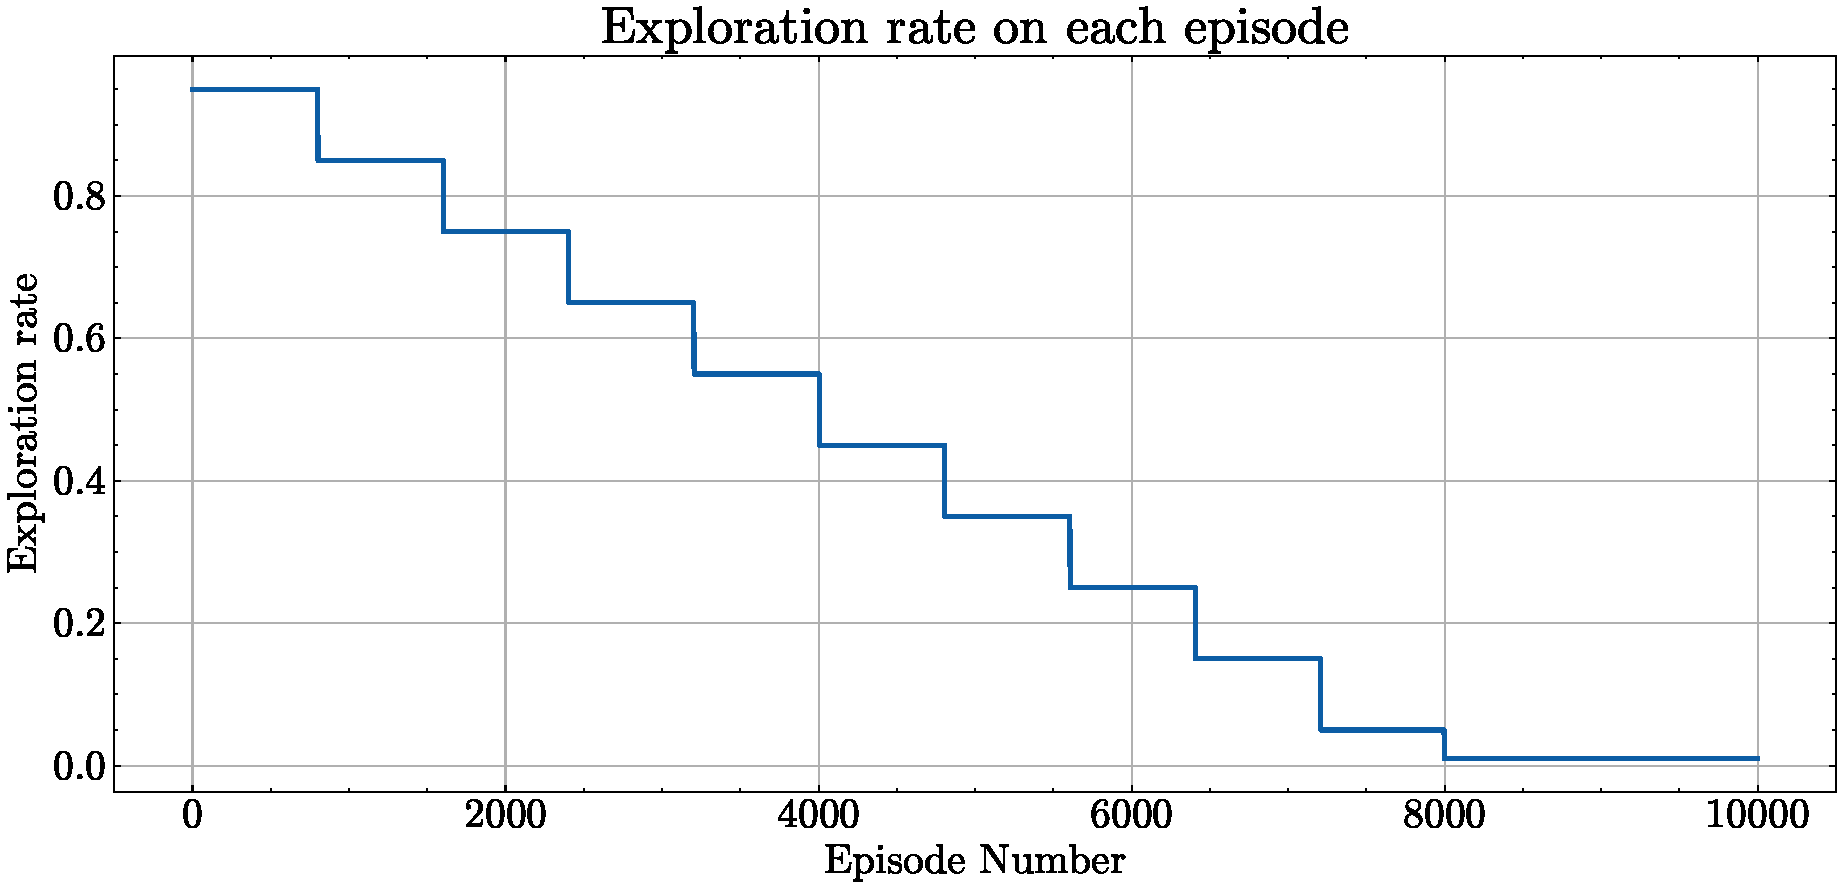
\includegraphics[height=6cm]{imagenes/cap4/adaptacion_trafico_qlearning/exploration_rate.pdf}
    \caption{Evolución del ratio de exploración del sigue carril con adaptación al tráfico}
    \label{fig:Evolución del ratio de exploración del sigue carril con adaptación de velocidad en función del tráfico}
\end{figure}
        
  \begin{figure}[h]
    \centering
    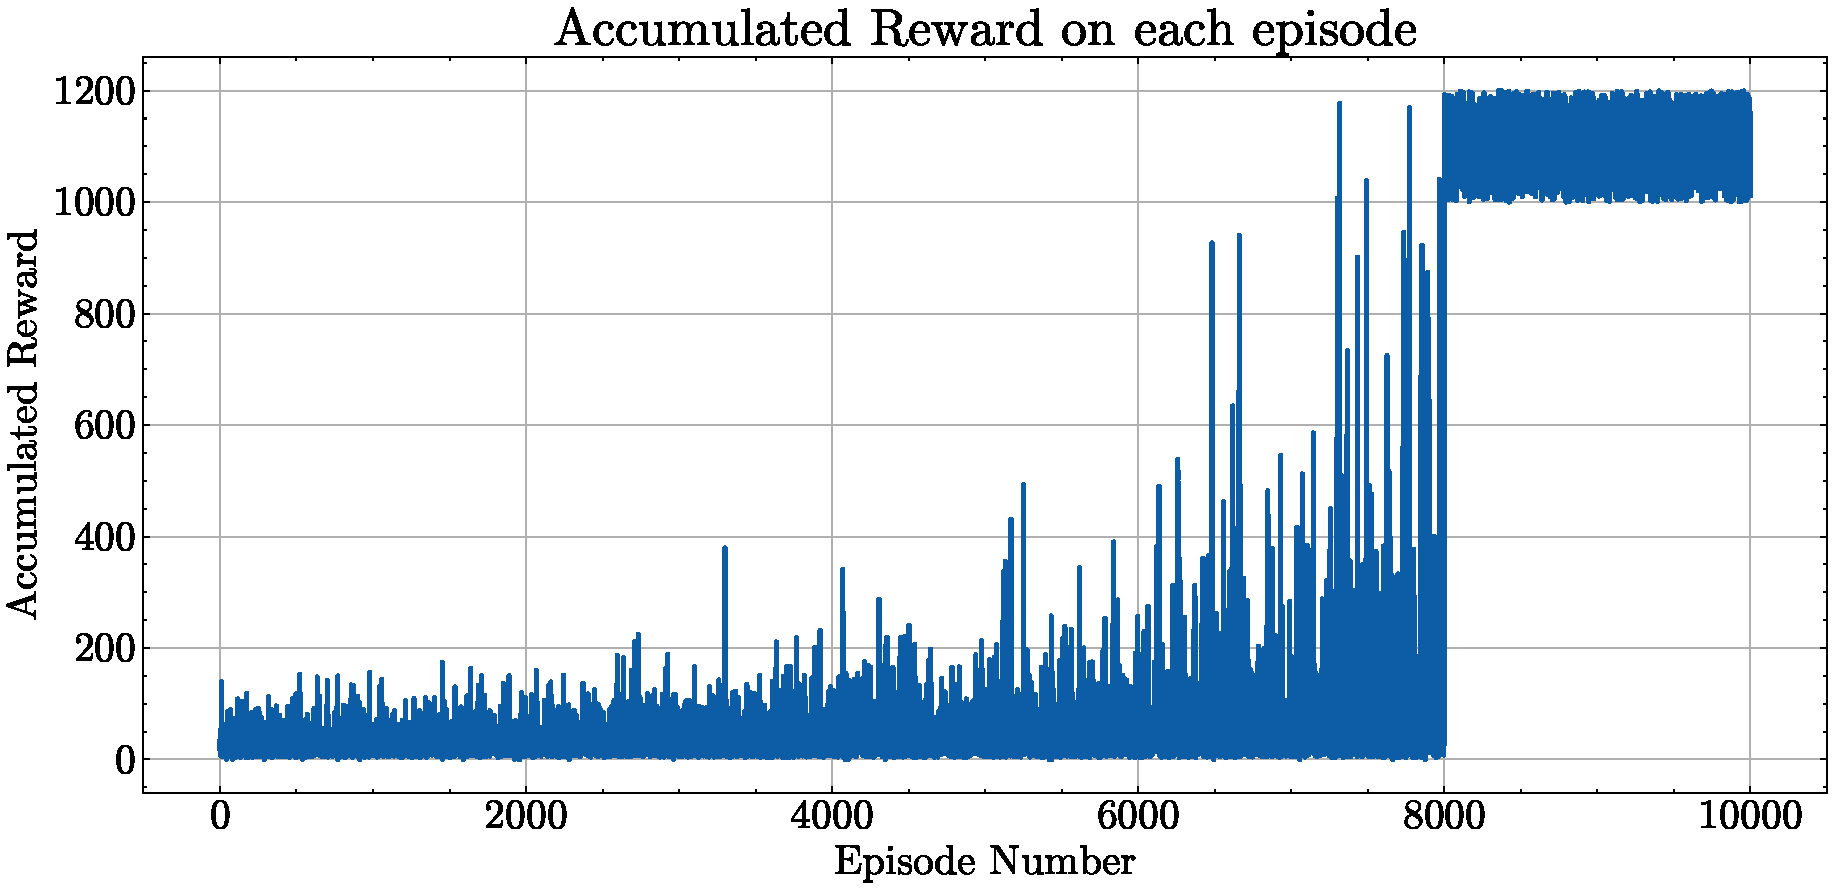
\includegraphics[height=6cm]{imagenes/cap4/adaptacion_trafico_qlearning/reward.pdf}
    \caption{Evolución de la recompensa acumulada del sigue carril con adaptación al tráfico}
    \label{fig:Evolución de la recompensa acumulada del sigue carril con adaptación de velocidad en función del tráfico}
\end{figure}

\bigskip

Para probar el funcionamiento  del modelo entrenado, el método elegido fue permitir al vehículo seguir el carril del circuito de entrenamiento que se puede ver en la figura \ref{fig:Entorno de entrenamiento del algoritmo de Q-learnig} con la modificación de que a mitad de trayecto se encontraría con otro vehículo que también estaría siguiendo el carril pero a una velocidad más reducida, el vehículo principal entonces tendría que adaptarse a la velocidad del vehículo más lento sin colisionar. Algo a destacar es que el vehículo que sigue el carril con una velocidad más lenta en esta prueba mencionada, es un vehículo normal de CARLA que se genera en un tramo avanzado de la vía y al cual se le carga el método de seguimiento de carril descrito en la sección \ref{Sigue carril} pero reentrenando el modelo con unas velocidades menores a las mostradas en su sección. Esto demuestra la robustez de este algoritmo, ofreciendo tan buenos resultados en el seguimiento de carril que incluso se ha podido utilizar para probar el funcionamiento de esta nueva implementación.

\bigskip

Tras varias pruebas del algoritmo con el método que se acaba de mencionar, podemos analizar la gráfica de acciones de la figura \ref{fig:Histograma de las acciones de giro tomadas por el agente de Qlearning en el método de adaptación al tráfico} nuevamente podemos comprobar que la mayoría de acciones de giro ejecutadas por nuestro agente son la ausencia de giro, dejado el volante si mover o con giros pequeños y favoreciendo así una conducción natural.


  \begin{figure}[h]
    \centering
    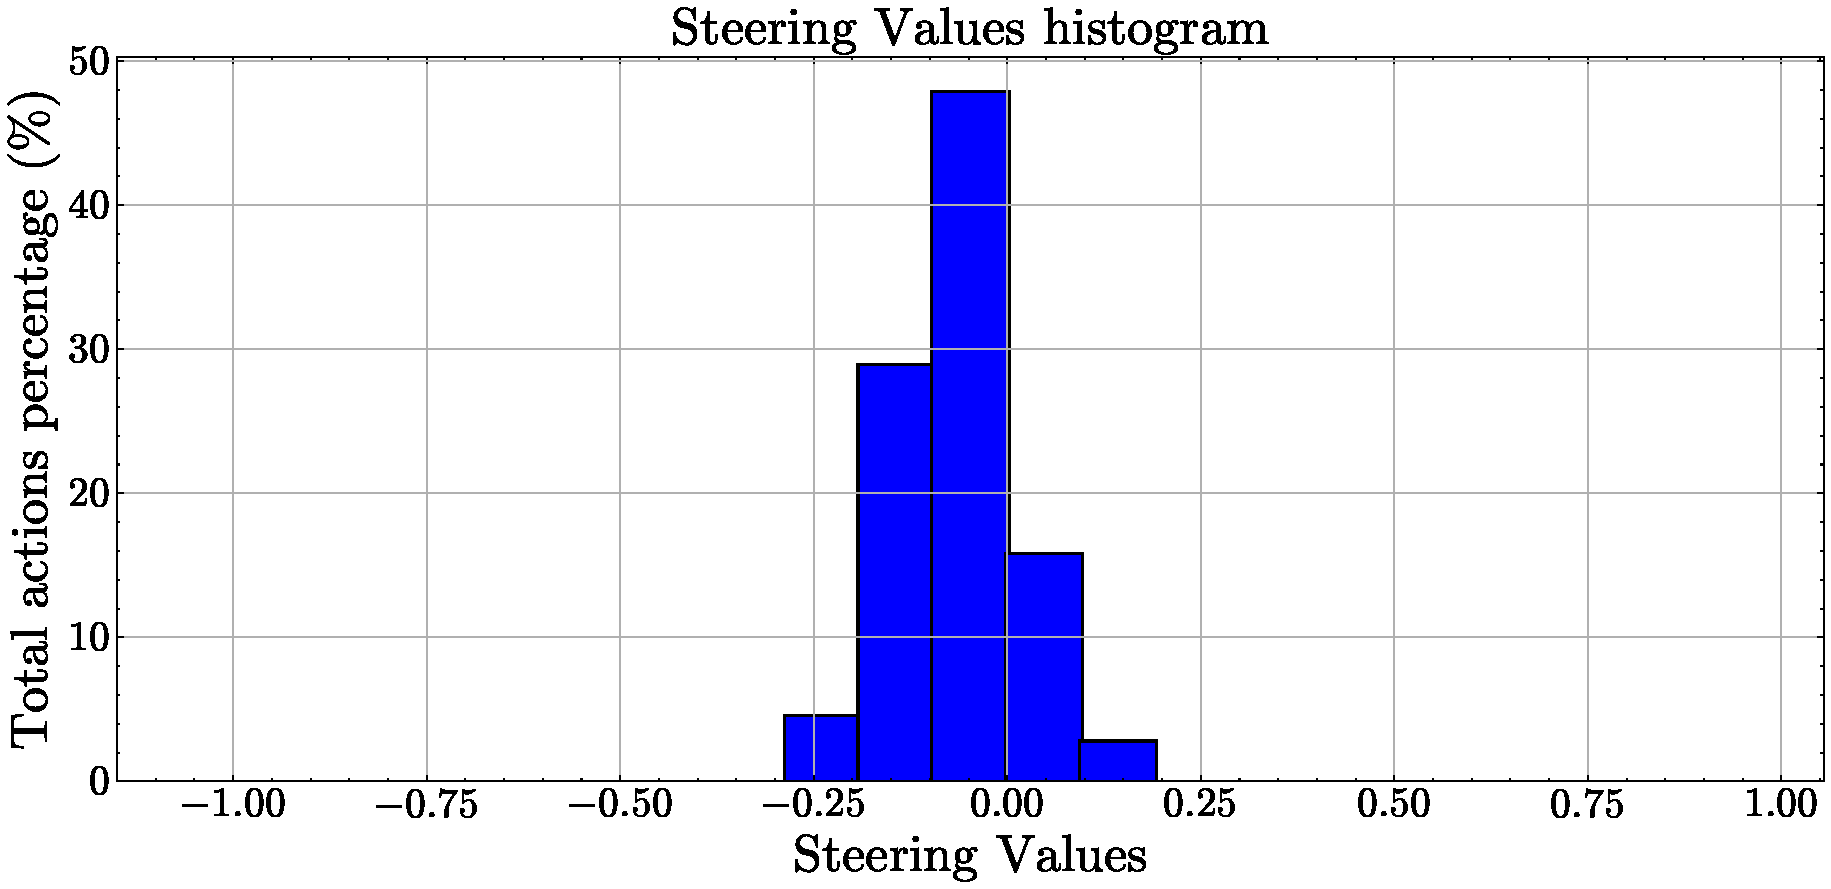
\includegraphics[height=6cm]{imagenes/cap4/adaptacion_trafico_qlearning/actions_traffic.pdf}
    \caption{Histograma de las acciones de giro tomadas por sigue carril con adaptación al tráfico}
    \label{fig:Histograma de las acciones de giro tomadas por el agente de Qlearning en el método de adaptación al tráfico}
\end{figure}

No obstante, nuevamente en la gráfica de velocidades de la figura \ref{fig:Histograma de las velocidades utilizadas por el agente de Qlearning en el método de adaptación al tráfico} podemos encontrar particularidades interesantes y es que como vemos ahora tenemos una variedad de velocidades muchos más grande que en anteriores casos, obviamente esto se debe a la reducción de velocidad que realiza nuestro agente cuando aparece tráfico más lento en la vía incluso llegando a detenerse en caso de que este lo haga. De esta manera podemos comprobar que efectivamente la implementación esta funcionando correctamente y el vehículo al encontrarse con tráfico esta reduciendo la velocidad e incluso frenando en caso de que así sea necesario.

  \begin{figure}[h]
    \centering
    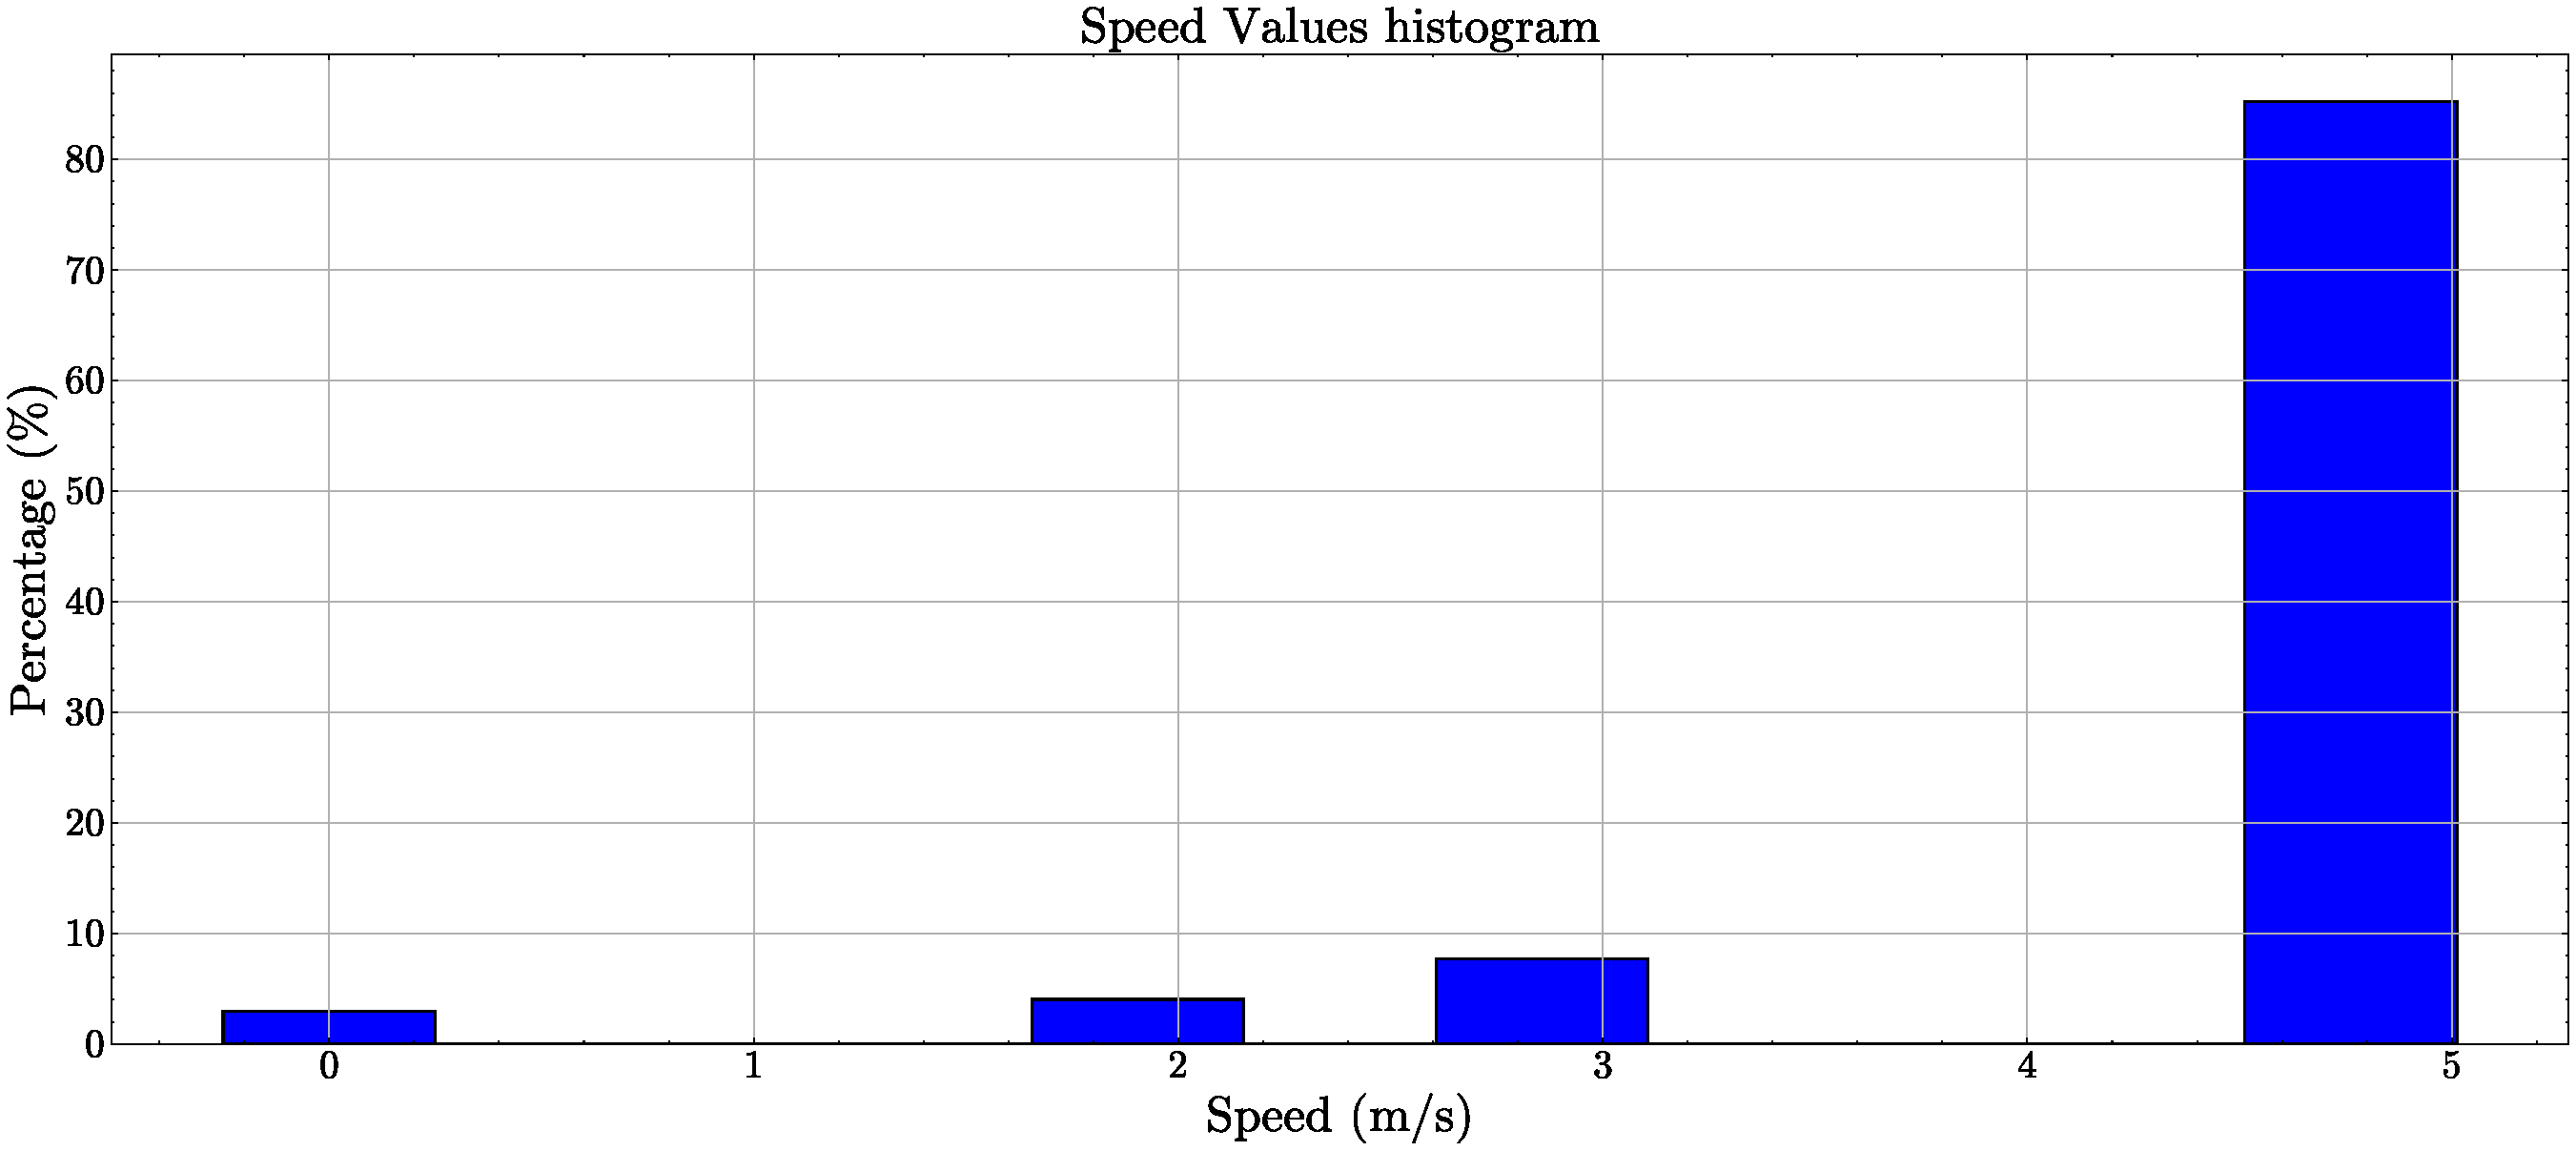
\includegraphics[height=6cm]{imagenes/cap4/adaptacion_trafico_qlearning/traffic_speeds.pdf}
    \caption{Histograma de las velocidades utilizadas por el sigue carril con adaptación al tráfico}
    \label{fig:Histograma de las velocidades utilizadas por el agente de Qlearning en el método de adaptación al tráfico}
\end{figure}


En figura \ref{fig:Sigue carriles con adaptación al trafico basado en Qlearning} podemos encontrar una serie de imágenes del funcionamiento de este método, si nos fijamos en la esquina superior derecha de cada imagen aparece le velocidad lineal del vehículo en cada momento, podemos observar como la velocidad lineal se suele mantener alrededor entre los 4.5 y los 5 m/s, en ausencia de tráfico pero cuando empezamos a circular por detrás del vehículo que aparece en el carril el cual navega a una velocidad mucho más lenta, la velocidad de nuestro vehículo principal se ve reducida y baja hasta los 2.7 m/s, adaptándose así a la velocidad reducida del vehículo de adelante a la vez que sigue el carril. Posteriormente el vehículo de adelante desaparece y nuestro agente retoma su velocidad normal hasta terminar el circuito. También podemos fijarnos que las velocidades el vehículo no llegar a ser siempre las comandadas por el algoritmo de Q-learning que se pueden explicadas en el código en la gráfica \ref{cod:Acciones disponibles para el algoritmo de qlearning con adaptación al tráfico}, esto se debe al hecho de que el control que nos ofrece CARLA sobre la velocidad del vehículo como ya se comento previamente es el empuje y no la velocidad lineal por eso el controlador presentado en el código \ref{cod:Controlador de velocidad fija del vehículo} regula la cantidad de empuje para intentar mantener la velocidad lo más cerca posible de la comandada por el algoritmo aplicando, sin embargo este controlador no llega a ser 100\% preciso y la velocidad el vehículo oscila alrededor del valor deseado.

\bigskip

  \begin{figure}[h]
    \centering
    \includegraphics[height=7cm]{imagenes/cap4/demostraciones_qlearning/traffic/demostracion_sigue_Carriles.pdf}
    \caption{Sigue carril con adaptación al trafico}
    \label{fig:Sigue carriles con adaptación al trafico basado en Qlearning}
\end{figure}

\newpage

Como conclusión los resultados del entrenamiento fueron nuevamente exitosos, obtuvimos un modelo capaz de conducir de manera fluida por un carril y que en caso de encontrarse con tráfico adaptarse a su velocidad llegando incluso a detener la marcha si así fuera necesario, sin embargo este comportamiento resulta muy complejo por lo que se ha tenido que emplear varias tablas Q y entrenar durante largos periodos de tiempo, probablemente aquí hayamos llegado al límite del algoritmo Q-learning y si buscáramos crear algún otro comportamiento incluso más complejo sería buena idea valorar otros métodos de \ac{IA} más sofisticados.
\bigskip

Para acabar en uno de los apartados de esta \href{https://roboticslaburjc.github.io/2022-tfg-juancamilo-carmona/DEMOS/}{\textbf{entrada}} del blog de este \ac{TFG} se puede encontrar un video demostración del funcionamiento de seguimiento de seguimiento de carril con adaptación al tráfico, siguiendo la prueba descrita anteriormente, donde veremos al vehículo navegar por el carril hasta encontrarse con otro vehículo equipado con el algorimto de carril de la sección \ref{Sigue carril} navegando a una velocidad reducida por lo que el vehículo principal tendrá que adaptarse a la velocidad de este sin llegar a colisionar.









\chapter{Conclusiones}
\label{cap:capitulo5}

En este \acs{TFG} se han tres objetivos principales: Primero la creación de una solución de conducción autónoma para el problema concreto de un seguimiento de carril, segundo comparar distintas técnicas de filtrado de carril, tanto basadas en visión artificial convencional como en inteligencia artificial, con el fin de evaluar sus ventajas y desventajas para determinar cuál es el método más eficaz. Tercero, analizar la viabilidad del desarrollo de aplicaciones de conducción autónoma utilizando el simulador foto-realista CARLA y el framework de robótica ROS 2 empleando como medio de comunicación el \textit{CARLA to ROS bridge}

Finalizamos este trabajo comentando los objetivos que se han cumplido a lo largo del desarrollo del proyecto, cómo se han satisfecho los requisitos expuestos en el capítulo \ref{cap:capitulo2}, así como posibles líneas futuras de investigación, englobando mejoras al proyecto propuesto.

\section{Objetivos cumplidos}
\label{sec:objetivos_cumplidos}

De los objetivos presentados en la sección \ref{sec:Objetivos}, todos ellos han sido logrados exitosamente
\begin{enumerate}
	\item Se  logró la instalación y configuración de CARLA y ROS 2, y se estableció una comunicación efectiva entre ambos utilizando el  \textit{CARLA to ROS bridge}
	
	\item Se llegó a una conclusión sobre la viabilidad de desarrollar aplicaciones de conducción autónoma mediante el uso del simulador foto-realista CARLA y el framework ROS 2, utilizando  \textit{CARLA to ROS bridge}  como medio de comunicacicón.
	
	\item Se implementó con éxito un sistema de seguimiento de carril usando aprendizaje por refuerzo y redes neuronales como métodos de control y percepción visual.
	
	\item Se diseñó un algoritmo de seguimiento de carril, con la funcionalidad añadida de frenar al encontrar obstáculos en la vía.
	
	\item Se desarrolló una implementación de conducción autónoma capaz de navegar por un carril adaptándose al flujo del tráfico mediante el uso de aprendizaje por refuerzo.
	
	\item Se han llevado a cabo análisis rigurosos para cada uno de los métodos de detección de carril y se contrastaron sus métricas de forma exitosa.
	
\end{enumerate}


\section{Requisitos satisfechos}
\label{sec:requisitos_satisfechos}

En cuanto a los requisitos solicitados a cumplir en el apartado \ref{sec:requisitos}, nuevamente todos ellos han sido satisfechos con éxito:
\begin{enumerate}
	\item Como se estableció, el trabajo se ha realizado enteramente en el simulador foto-realista de conducción autónoma CARLA.
	\item Todos los que se han desarrollado han sido reactivos, a pesar de las limitaciones de \ac{FPS} encontradas.
	\item En todos los algoritmos vehículo ha navegado de manera adecuada, natural y segura.
\end{enumerate}

\section{Balance global y competencias adquiridas}
\label{sec:balance_global_competencias_adquiridas}


En este \ac{TFG} se han logrado avances altamente positivos en varios frentes del desarrollo y la investigación en el campo de la conducción autónoma. Se han implementado múltiples técnicas para el seguimiento de carriles, incluyendo desde enfoques más tradicionales hasta métodos más actuales que hacen uso de la inteligencia artificial. Esto no solo ha enriquecido la comprensión de los sistemas de seguimiento de carriles, sino que también ha permitido una comparativa profunda de la eficacia de distintas estrategias.

\bigskip

Más allá del seguimiento de carriles, se ha avanzado en crear soluciones de conducción autónoma con comportamientos más complejos. Los algoritmos finales desarrollados son capaces de detener el vehículo al encontrar obstáculos y adaptar su velocidad si dichos obstáculos están en movimiento, lo que añade una capa adicional de robustez y versatilidad al sistema.

\bigskip

Adicionalmente, se ha profundizado en la sinergia entre ROS 2 y el simulador CARLA, lo que ha abierto un amplio abanico de posibilidades para la creación de aplicaciones de conducción autónoma en ROS 2, pero también ha expuesto algunas limitaciones que deben ser consideradas en caso de querer llevar estas aplicaciones más haya de la fase de prototipo. Esta experiencia ha proporcionado una visión realista y práctica de cómo estas dos plataformas pueden interactuar, destacando tanto sus ventajas como sus inconvenientes.

\bigskip

Finalmente, el proyecto ha servido como una incursión significativa en el campo de la inteligencia artificial aplicada a la conducción autónoma. Se ha evidenciado que esta tecnología, en constante evolución, tiene un gran potencial para superar muchos de los desafíos actuales en este ámbito. Su capacidad para aprender y adaptarse a distintas situaciones  la convierte en una herramienta extremadamente poderosa para el desarrollo de sistemas de transporte más seguros, eficientes y rápidos.

\bigskip


A lo largo del desarrollo de este trabajo, se han ido adquiriendo una serie de habilidades y competencias, entre las que se incluyen:
\begin{itemize}
	\item Organización del tiempo y trabajo.
	\item Resolución de problemas durante las reuniones.
	\item Familiarización con la metodología de trabajo scrum 
	\item Aumento general de la destreza en la programación.
	\item Gran aumento de destreza y conocimiento en el uso de redes neuronales
	\item Gran aumento de destreza y conocimiento en la implementación y uso de técnicas de aprendizaje por refuerzo
	\item Mejora en la capacidad para desarrollar algoritmos de visión artificial y en el procesamiento de imágenes
	\item Avance significativo en la maestría de ROS 2 y su integración con aplicaciones externas
	\item Mejora en la competencia y entendimiento para el desarrollo de aplicaciones de conducción autónoma
\end{itemize}

\section{Líneas futuras}
\label{sec:lineas_futuras}

A pesar de que todos los objetivos de este proyecto se han logrado satisfactoriamente, la conducción autónoma es un mundo muy amplio y varias líneas de investigación podrían nacer a partir de este \ac{TFG}.
\begin{enumerate}
	\item Mejora de los sistemas de seguimiento de carril finales utilizando enfoques de aprendizaje por refuerzo más sofisticados sin las limitaciones propias del algoritmo de Q-learning
	\item Exploración de otros métodos de \ac{IA} como deep learning o imitation learning para el control del vehículo en sustitución de Q-learning
	\item Ampliación de las funcionalidades del sistema final de sigue carril con adaptación al tráfico: funcionalidad para adelantar, para cambios de carril, para reconocimiento de intersecciones etc.
	\item Búsqueda de una solución para el cuello de botella generado en los \ac{FPS} de programas desarrollados utilizando el \textit{CARLA to ROS bridge} para así migrar las implementaciones finales de la \ac{API} de CARLA a ROS 2
	\item Testear este \ac{TFG} en escenarios distintos, con mas tráfico, con situaciones meteorológicas adversas etc.
\end{enumerate}




\chapter{Anexo}
\label{cap:anexo}

A continuación se muestran las referencias a las figuras de este trabajo junto con la fuente de la que han sido obtenidas:

%|m{3cm}|p{9cm}|

\begin{table}[H]
\begin{center}
\begin{tabular}{|p{0.3\textwidth}|p{0.7\textwidth}|}
\hline
\textbf{Referencia imágenes} & \textbf{Fuente de la que se ha obtenido}\\

\hline

\ref{fig:Disciplinas que componen la robótica.} & \textbf{1.}\url{https://informaticai2015.wordpress.com/2015/10/13/robotica/} \\


\hline

\ref{fig:Ilustración de un robot móvil generado por IA} & \textbf{1.}\url{https://www.bing.com/images/create} \\


\hline

\ref{Ilustración de coches autónomos generada por IA} & \url{https://www.bing.com/images/create} \\

\hline

\ref{fig:Niveles de conducción autónoma según el estándar J3016} &  \href{https://www.motor.es/noticias/con-el-nivel-3-de-conduccion-autonoma-conduces-pero-menos-202072774.html}{\textbf{https://www.motor.es/noticias/con-el-nivel-3-de-conduccion-autonoma}} \\

\hline

\ref{fig:Vehículo tesla}  & \url{https://www.topgear.es/noticias/garaje/tesla-model-s-coupe-90776} \\

\hline

\ref{fig:robotaxi} & \url{https://www.theverge.com/2022/11/21/23471183/waymo-zeekr-geely-autonomous-vehicle-av-robotaxi} \\

\hline

\ref{fig:Ilustración de una red neuronal} & \href{https://www.researchgate.net/figure/Figura-1-Conceptualizacion-de-una-red-neuronal-artificial-como-un-sistema-Figure-1_fig1_335360392}{https://www.researchgate.net} \\

\hline


\ref{fig:Ilustración de la metodología scrum} & \href{https://medium.com/@francoismugorozi/my-understanding-of-the-scrum-framework-and-benefits-of-the-scrum-events-ebd889da1472}{https://medium.com/@francoismugoroz} \\

\hline


\ref{fig:CARLA_vehicles} & {\url{https://carla.org/2020/12/22/release-0.9.11/}} \\

\hline

\ref{fig:Ros2_logos} &  \url{https://foxglove.dev/blog/the-building-blocks-of-ros2} \\

\hline

\ref{fig:carla_to_ros_bridge} & \href{https://discourse.ros.org/t/thoughts-on-ignition-gazebo-simulator-and-ros2-bridge/16477}{https://discourse.ros.org} \\

\hline

\ref{fig:vcs logo} & \url{https://gerardorenteria.blog/2023/10/05/visual-studio-code-version-updated/} \\

\hline

\ref{fig:logotipo_ros_2_foxy} & \url{https://discourse.ros.org/t/ros-foxy-fitzroy-released/14495} \\

\hline

\end{tabular}
\caption{Anexo con las fuentes de donde se han obtenido las imágenes para este proyecto}
\label{cuadro:anexo_imagenes_fuentes}
\end{center}
\end{table}




\chapter*{Epilogo}
\label{cap:Epilogo}

\textit{Como ingeniero en robótica software, creo firmemente que la inteligencia artificial es una de las herramientas más increíbles que ha surgido en toda la historia de la humanidad. Los avances que hemos visto, especialmente en los últimos años, son más que impresionantes y no dejan a nadie indiferente. Las nuevas aplicaciones que van apareciendo día a día muestran claramente el gran potencial de esta tecnología y la herramienta tan útil que constituye. Aunque hay quienes la rechazan, bajo mi punto de vista es seguro que en el futuro la inteligencia artificial en todas sus vertientes acabará formando parte integral de nuestra sociedad, favoreciendo al avance del ser humano como especie, tal y como ocurrió en su momento con internet, con la maquina a vapor en la revolución industrial y con todos los grandes hitos de la ciencia y la ingenieria de nuestra historia.}

\bigskip

\textit{De la misma manera que en este TFG he utilizado distintas técnicas de inteligencia artificial para lograr el desarrollo de los algoritmos y soluciones de conducción autónoma, también he utilizado distintas herramientas de inteligencia artificial para la realización del mismo. Algunas de las ilustraciones que en esta memoria se presentan las he creado con inteligencias artificiales de generación de imágenes, además durante el desarrollo de toda la memoria y del TFG en si he utilizado distintas herramientas procesamiento y generación de texto basadas en inteligencia artificial como herramientas de apoyo para: correcciones ortográficas, correcciones gramaticales, ordenamiento de ideas, investigación de información, generación de código etc. Porque si nosotros, los ingenieros en robótica e inteligencia artificial que amamos y dedicamos nuestra vida a estos campos no confiamos y utilizamos nuestra propia tecnología, ¿quién va a hacerlo?}

\bigskip

\begin{quote}
    ``Algunas personas llaman a esto inteligencia artificial, pero la realidad es que esta tecnología nos mejorará. Entonces, en lugar de inteligencia artificial, creo que aumentaremos nuestra inteligencia.''
    \hfill ---Ginni Rometty
\end{quote}

\bigskip


\printindex \nocite{*}
\appendix

\bibliographystyle{unsrt}

\bibliography{bibliografia}

\newpage
\thispagestyle{empty}

\vspace*{\fill}

\begin{figure}[!h] 
    \centering
    \includegraphics[width=1\linewidth]{imagenes/Chinche_y_yo.jpeg} 
\end{figure}

\vspace*{\fill}

\begin{flushright}
    \par
    \vspace{1.0 cm}
    \emph{Dedicado a Jairo Mejía Gutiérrez (Chinche)}
\end{flushright}

\end{document}

